% Options for packages loaded elsewhere
% Options for packages loaded elsewhere
\PassOptionsToPackage{unicode}{hyperref}
\PassOptionsToPackage{hyphens}{url}
%
\documentclass[
  letterpaper,
]{book}
\usepackage{xcolor}
\usepackage{amsmath,amssymb}
\setcounter{secnumdepth}{5}
\usepackage{iftex}
\ifPDFTeX
  \usepackage[T1]{fontenc}
  \usepackage[utf8]{inputenc}
  \usepackage{textcomp} % provide euro and other symbols
\else % if luatex or xetex
  \usepackage{unicode-math} % this also loads fontspec
  \defaultfontfeatures{Scale=MatchLowercase}
  \defaultfontfeatures[\rmfamily]{Ligatures=TeX,Scale=1}
\fi
\usepackage{lmodern}
\ifPDFTeX\else
  % xetex/luatex font selection
\fi
% Use upquote if available, for straight quotes in verbatim environments
\IfFileExists{upquote.sty}{\usepackage{upquote}}{}
\IfFileExists{microtype.sty}{% use microtype if available
  \usepackage[]{microtype}
  \UseMicrotypeSet[protrusion]{basicmath} % disable protrusion for tt fonts
}{}
\makeatletter
\@ifundefined{KOMAClassName}{% if non-KOMA class
  \IfFileExists{parskip.sty}{%
    \usepackage{parskip}
  }{% else
    \setlength{\parindent}{0pt}
    \setlength{\parskip}{6pt plus 2pt minus 1pt}}
}{% if KOMA class
  \KOMAoptions{parskip=half}}
\makeatother
% Make \paragraph and \subparagraph free-standing
\makeatletter
\ifx\paragraph\undefined\else
  \let\oldparagraph\paragraph
  \renewcommand{\paragraph}{
    \@ifstar
      \xxxParagraphStar
      \xxxParagraphNoStar
  }
  \newcommand{\xxxParagraphStar}[1]{\oldparagraph*{#1}\mbox{}}
  \newcommand{\xxxParagraphNoStar}[1]{\oldparagraph{#1}\mbox{}}
\fi
\ifx\subparagraph\undefined\else
  \let\oldsubparagraph\subparagraph
  \renewcommand{\subparagraph}{
    \@ifstar
      \xxxSubParagraphStar
      \xxxSubParagraphNoStar
  }
  \newcommand{\xxxSubParagraphStar}[1]{\oldsubparagraph*{#1}\mbox{}}
  \newcommand{\xxxSubParagraphNoStar}[1]{\oldsubparagraph{#1}\mbox{}}
\fi
\makeatother


\usepackage{longtable,booktabs,array}
\usepackage{calc} % for calculating minipage widths
% Correct order of tables after \paragraph or \subparagraph
\usepackage{etoolbox}
\makeatletter
\patchcmd\longtable{\par}{\if@noskipsec\mbox{}\fi\par}{}{}
\makeatother
% Allow footnotes in longtable head/foot
\IfFileExists{footnotehyper.sty}{\usepackage{footnotehyper}}{\usepackage{footnote}}
\makesavenoteenv{longtable}
\usepackage{graphicx}
\makeatletter
\newsavebox\pandoc@box
\newcommand*\pandocbounded[1]{% scales image to fit in text height/width
  \sbox\pandoc@box{#1}%
  \Gscale@div\@tempa{\textheight}{\dimexpr\ht\pandoc@box+\dp\pandoc@box\relax}%
  \Gscale@div\@tempb{\linewidth}{\wd\pandoc@box}%
  \ifdim\@tempb\p@<\@tempa\p@\let\@tempa\@tempb\fi% select the smaller of both
  \ifdim\@tempa\p@<\p@\scalebox{\@tempa}{\usebox\pandoc@box}%
  \else\usebox{\pandoc@box}%
  \fi%
}
% Set default figure placement to htbp
\def\fps@figure{htbp}
\makeatother





\setlength{\emergencystretch}{3em} % prevent overfull lines

\providecommand{\tightlist}{%
  \setlength{\itemsep}{0pt}\setlength{\parskip}{0pt}}



 


\makeatletter
\@ifpackageloaded{bookmark}{}{\usepackage{bookmark}}
\makeatother
\makeatletter
\@ifpackageloaded{caption}{}{\usepackage{caption}}
\AtBeginDocument{%
\ifdefined\contentsname
  \renewcommand*\contentsname{Table of contents}
\else
  \newcommand\contentsname{Table of contents}
\fi
\ifdefined\listfigurename
  \renewcommand*\listfigurename{List of Figures}
\else
  \newcommand\listfigurename{List of Figures}
\fi
\ifdefined\listtablename
  \renewcommand*\listtablename{List of Tables}
\else
  \newcommand\listtablename{List of Tables}
\fi
\ifdefined\figurename
  \renewcommand*\figurename{Figure}
\else
  \newcommand\figurename{Figure}
\fi
\ifdefined\tablename
  \renewcommand*\tablename{Table}
\else
  \newcommand\tablename{Table}
\fi
}
\@ifpackageloaded{float}{}{\usepackage{float}}
\floatstyle{ruled}
\@ifundefined{c@chapter}{\newfloat{codelisting}{h}{lop}}{\newfloat{codelisting}{h}{lop}[chapter]}
\floatname{codelisting}{Listing}
\newcommand*\listoflistings{\listof{codelisting}{List of Listings}}
\makeatother
\makeatletter
\makeatother
\makeatletter
\@ifpackageloaded{caption}{}{\usepackage{caption}}
\@ifpackageloaded{subcaption}{}{\usepackage{subcaption}}
\makeatother
\usepackage{bookmark}
\IfFileExists{xurl.sty}{\usepackage{xurl}}{} % add URL line breaks if available
\urlstyle{same}
\hypersetup{
  pdftitle={AI-NEPI Conference Proceedings - Enhanced Edition},
  pdfauthor={AI-NEPI Project Team},
  hidelinks,
  pdfcreator={LaTeX via pandoc}}


\title{AI-NEPI Conference Proceedings - Enhanced Edition}
\author{AI-NEPI Project Team}
\date{2025-01-01}
\begin{document}
\frontmatter
\maketitle
\begin{abstract}
This document serves as the main index for the AI-NEPI Conference
Proceedings. It provides an overview of the enhanced edition, which
contains presentations on Large Language Models for History, Philosophy
and Sociology of Science, held in 2025. The proceedings include
structured presentation content, slide images, speaker abstracts, and
detailed transcriptions.
\end{abstract}

\renewcommand*\contentsname{Table of contents}
{
\setcounter{tocdepth}{2}
\tableofcontents
}

\mainmatter
\bookmarksetup{startatroot}

\chapter{AI-NEPI Conference Proceedings - Enhanced
Edition}\label{ai-nepi-conference-proceedings---enhanced-edition}

This document serves as the main index for the AI-NEPI Conference
Proceedings. It provides an overview of the enhanced edition, which
contains presentations on Large Language Models for History, Philosophy
and Sociology of Science, held in 2025. The proceedings include
structured presentation content, slide images, speaker abstracts, and
detailed transcriptions.

\hfill\break

\bookmarksetup{startatroot}

\chapter{Preface}\label{preface}

This enhanced edition of the AI-NEPI Conference Proceedings contains
presentations on Large Language Models for History, Philosophy and
Sociology of Science, held in 2025.

The chapters in this book have been generated from comprehensive XML
content reports, providing structured access to the rich discussions and
insights shared during the conference.

Each chapter includes:

\begin{itemize}
\tightlist
\item
  Structured presentation content with key sections
\item
  Slide images synchronized with the presentation flow\\
\item
  Complete speaker abstracts and overviews
\item
  Detailed transcriptions of the presentations
\end{itemize}

This enhanced format allows readers to follow both the visual
presentation materials and the detailed content in an integrated manner.

\bookmarksetup{startatroot}

\chapter{Large Language Models for the History, Philosophy and Sociology
of Science
(Workshop)}\label{large-language-models-for-the-history-philosophy-and-sociology-of-science-workshop}

\bookmarksetup{startatroot}

\chapter*{Overview}\label{overview}
\addcontentsline{toc}{chapter}{Overview}

\markboth{Overview}{Overview}

\bookmarksetup{startatroot}

\chapter{---}\label{section}

\bookmarksetup{startatroot}

\chapter{---}\label{section-1}

\bookmarksetup{startatroot}

\chapter{Genre Classification for Historical Medical
Periodicals}\label{genre-classification-for-historical-medical-periodicals}

\bookmarksetup{startatroot}

\chapter*{Overview}\label{overview-1}
\addcontentsline{toc}{chapter}{Overview}

\markboth{Overview}{Overview}

This chapter delves into the ActDisease project, exploring its
objectives, the dataset of historical medical periodicals it employs,
and the inherent challenges encountered during dataset digitisation.
Subsequently, it details a series of genre classification experiments.
These experiments encompass the motivation behind genre classification,
an examination of zero-shot and few-shot classification techniques, and
specific trials involving few-shot prompting with the Llama-3.1 8b
Instruct model. The chapter culminates in a conclusion that synthesises
the findings and their implications.

\begin{figure}[H]

{\centering \pandocbounded{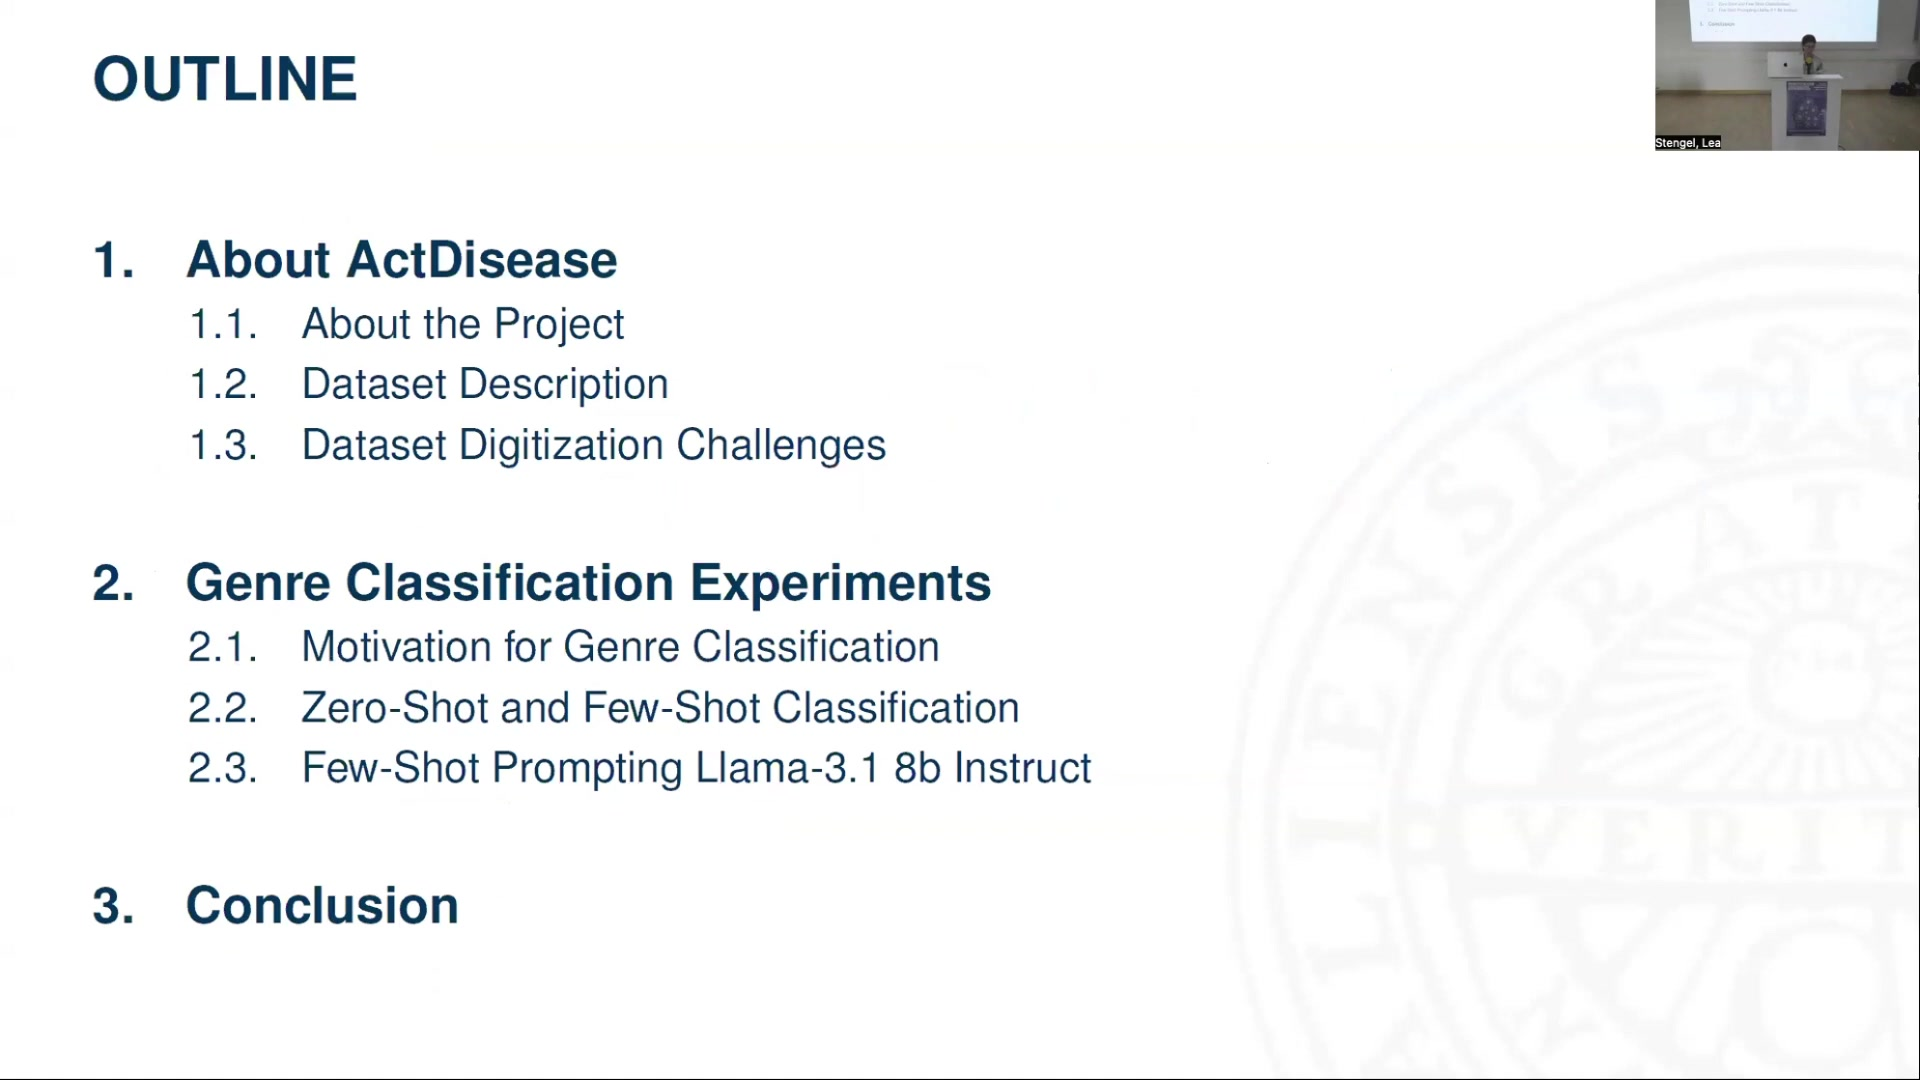
\includegraphics[keepaspectratio]{images/ai-nepi_005_slide_02.jpg}}

}

\caption{Outline of the chapter content, detailing sections on
ActDisease, Genre Classification Experiments, and Conclusion.}

\end{figure}%

\section{About ActDisease}\label{about-actdisease}

The ActDisease project, an initiative funded by the European Research
Council (ERC), investigates the histories of patient organisations
across Europe. Central to this research are the periodicals published by
these organisations in England, Germany, France, and Great Britain.
These documents serve as the primary source material for understanding
the evolution and impact of patient advocacy.

\begin{figure}[H]

{\centering \pandocbounded{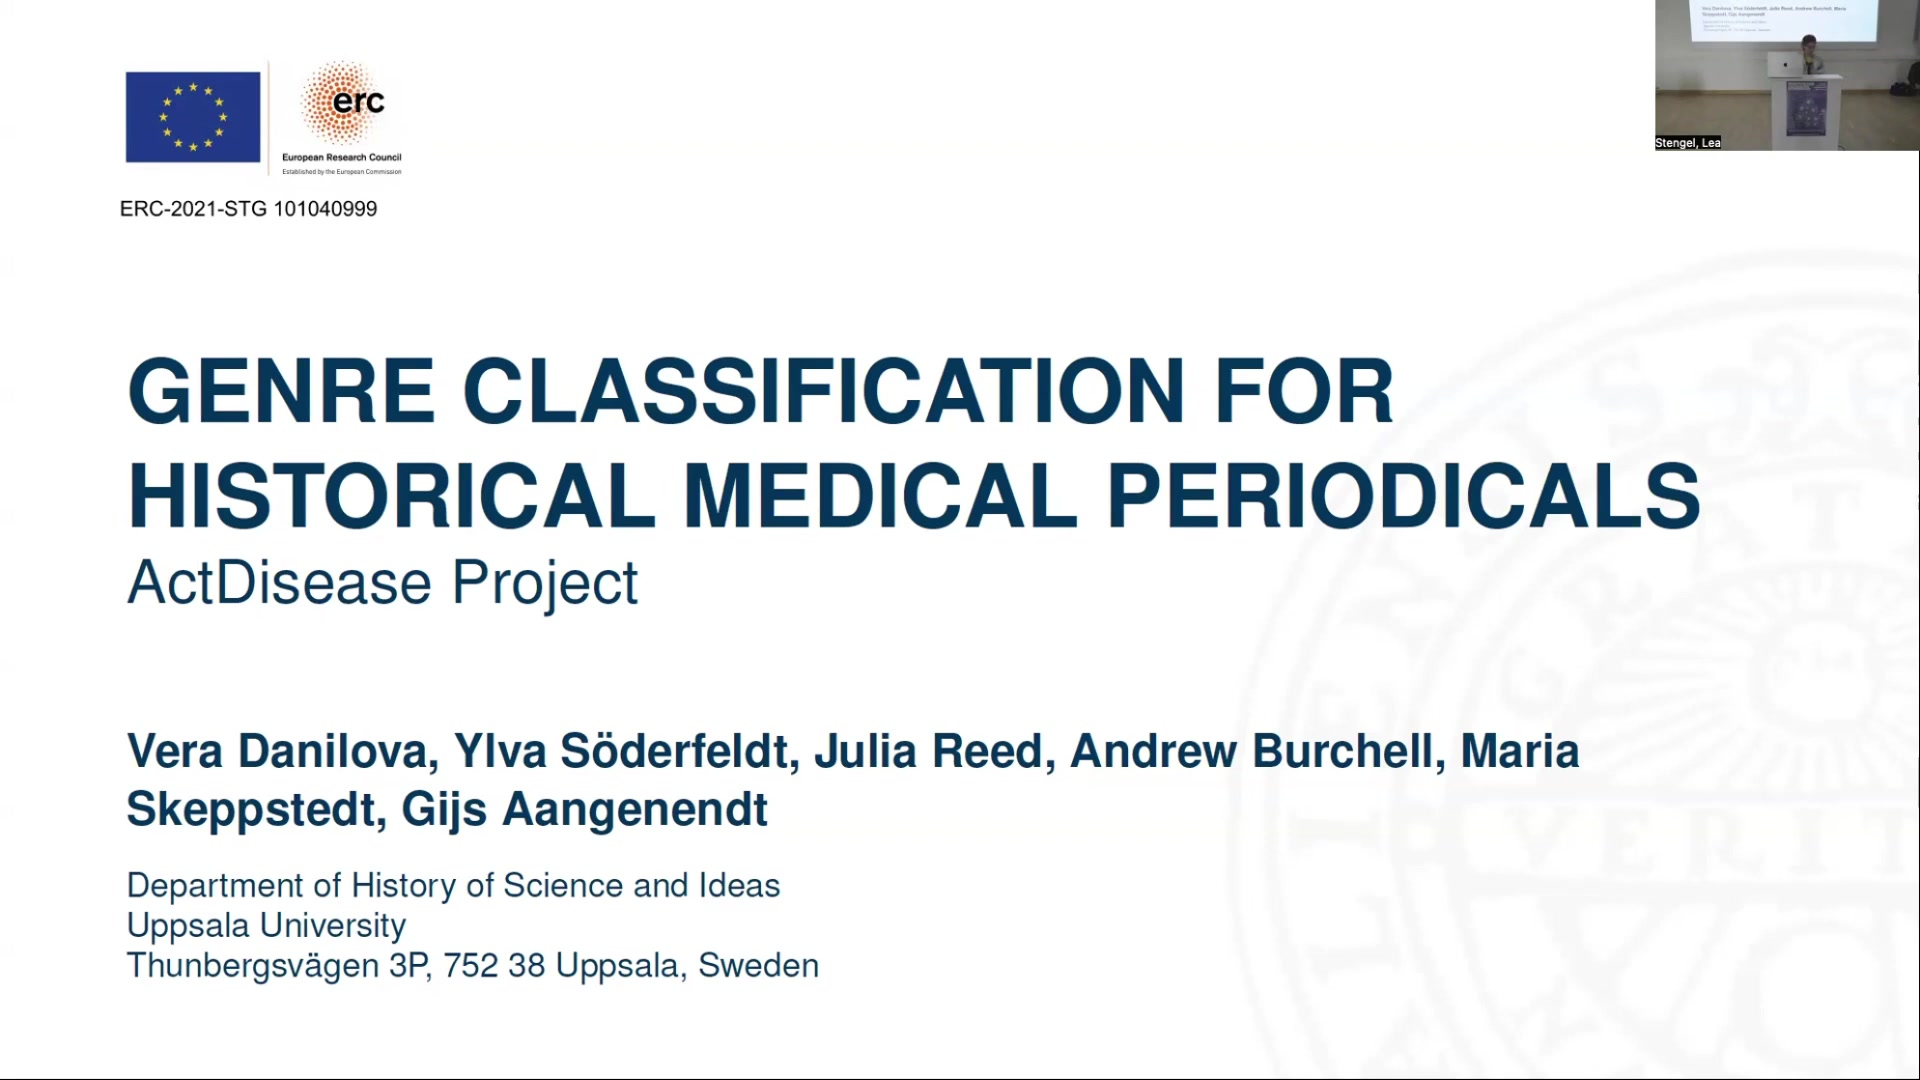
\includegraphics[keepaspectratio]{images/ai-nepi_005_slide_01.jpg}}

}

\caption{Title slide of the presentation `GENRE CLASSIFICATION FOR
HISTORICAL MEDICAL PERIODICALS', ActDisease Project, listing authors and
affiliation.}

\end{figure}%

\subsection{About the Project}\label{about-the-project}

ActDisease, an acronym for `Acting out Disease -- How Patient
Organizations Shaped Modern Medicine', is an ERC-funded research
endeavour. Its core purpose is to study how patient organisations in
20th-century Europe contributed to shaping disease concepts, illness
experiences, and medical practices. The project focuses on ten European
patient organisations from Sweden, Germany, France, and Great Britain,
covering a period from approximately 1890 to 1990. The principal source
materials are the periodicals, mostly magazines, produced by these
patient organisations.

\begin{figure}[H]

{\centering \pandocbounded{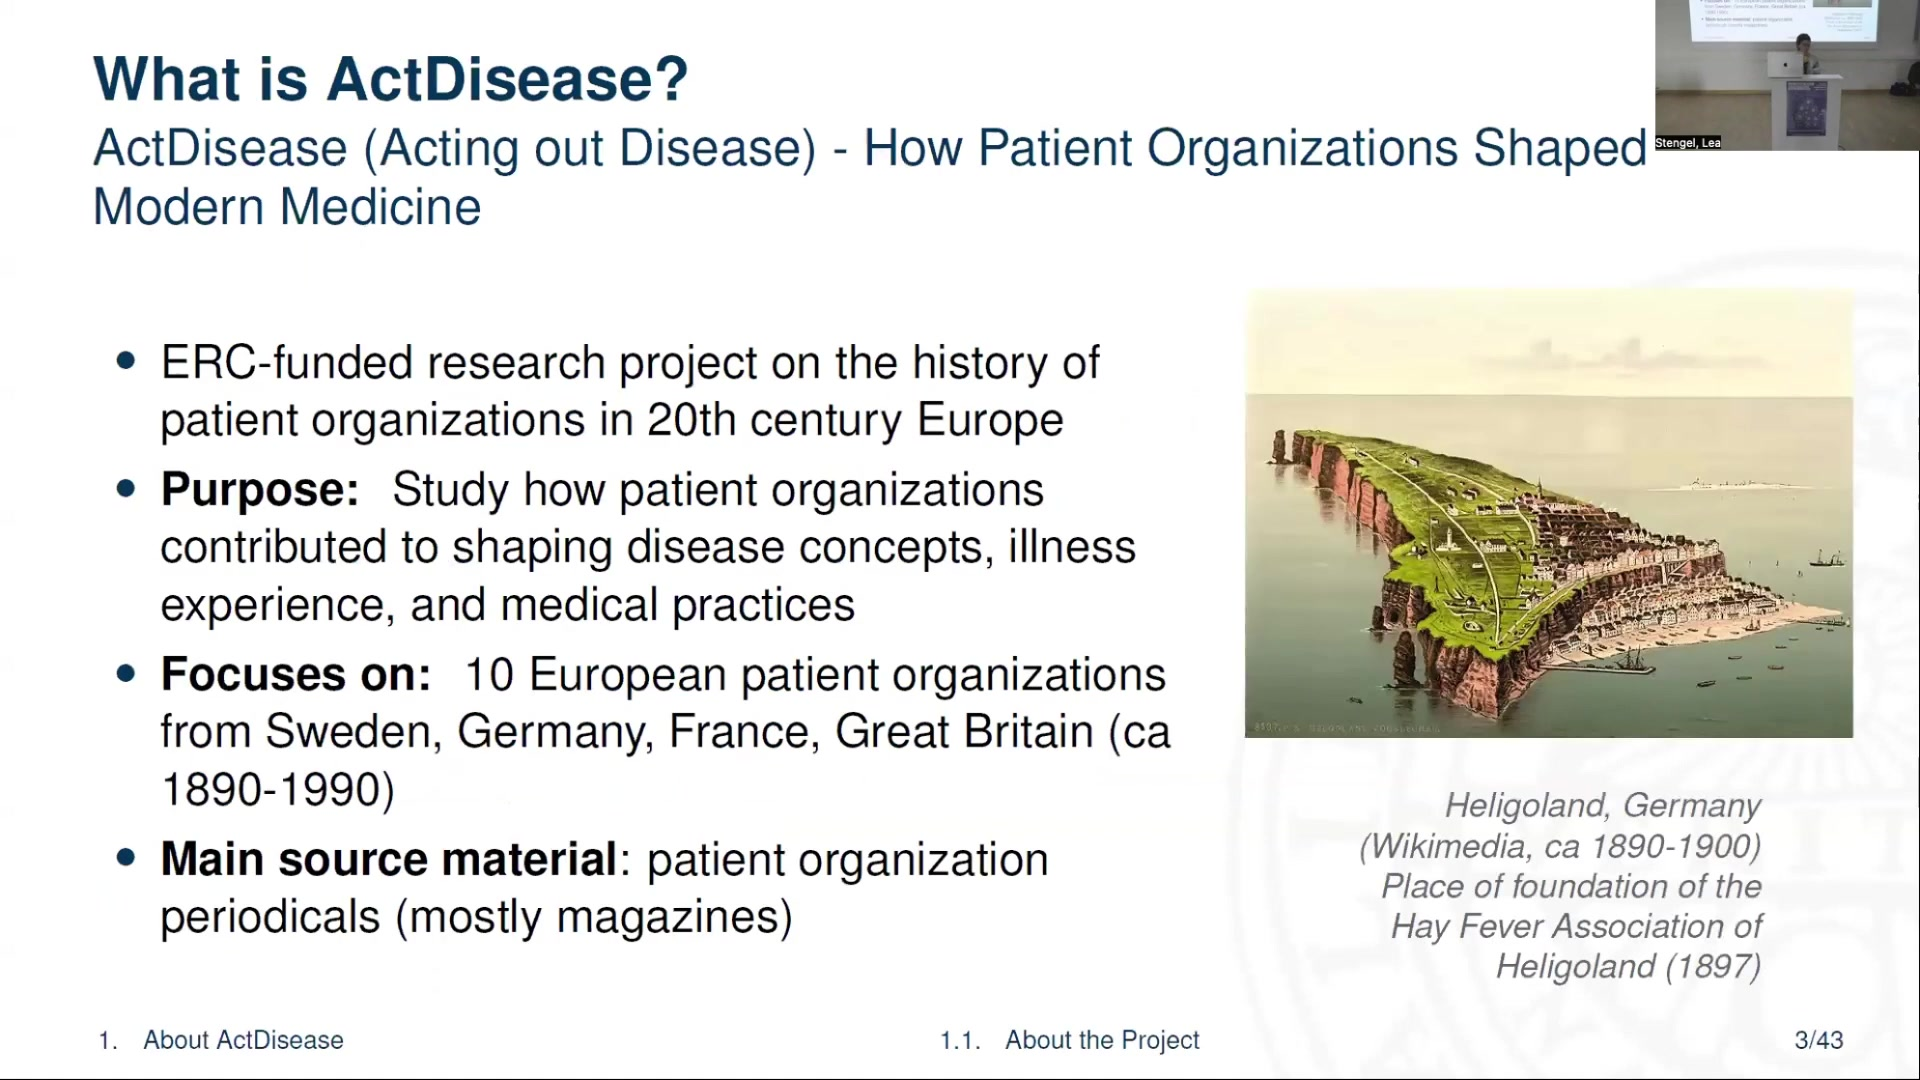
\includegraphics[keepaspectratio]{images/ai-nepi_005_slide_03.jpg}}

}

\caption{Slide describing the ActDisease project: its funding, purpose,
focus, and main source material, with an image of Heligoland, Germany.}

\end{figure}%

\subsection{Dataset Description}\label{dataset-description}

The ActDisease dataset comprises a private, recently digitised
collection of patient organisation magazines. This collection
encompasses materials from Germany, Sweden, France, and the United
Kingdom, covering diseases such as allergy/asthma, diabetes, multiple
sclerosis, lung diseases, and rheumatism/paralysis. The accompanying
image displays a table that summarises the magazines by country,
disease, total page count, and year coverage, amounting to 96,186 pages
in total. Initial explorations reveal a diverse array of text types
within these materials, with notable similarities in content across all
magazines.

\begin{figure}[H]

{\centering \pandocbounded{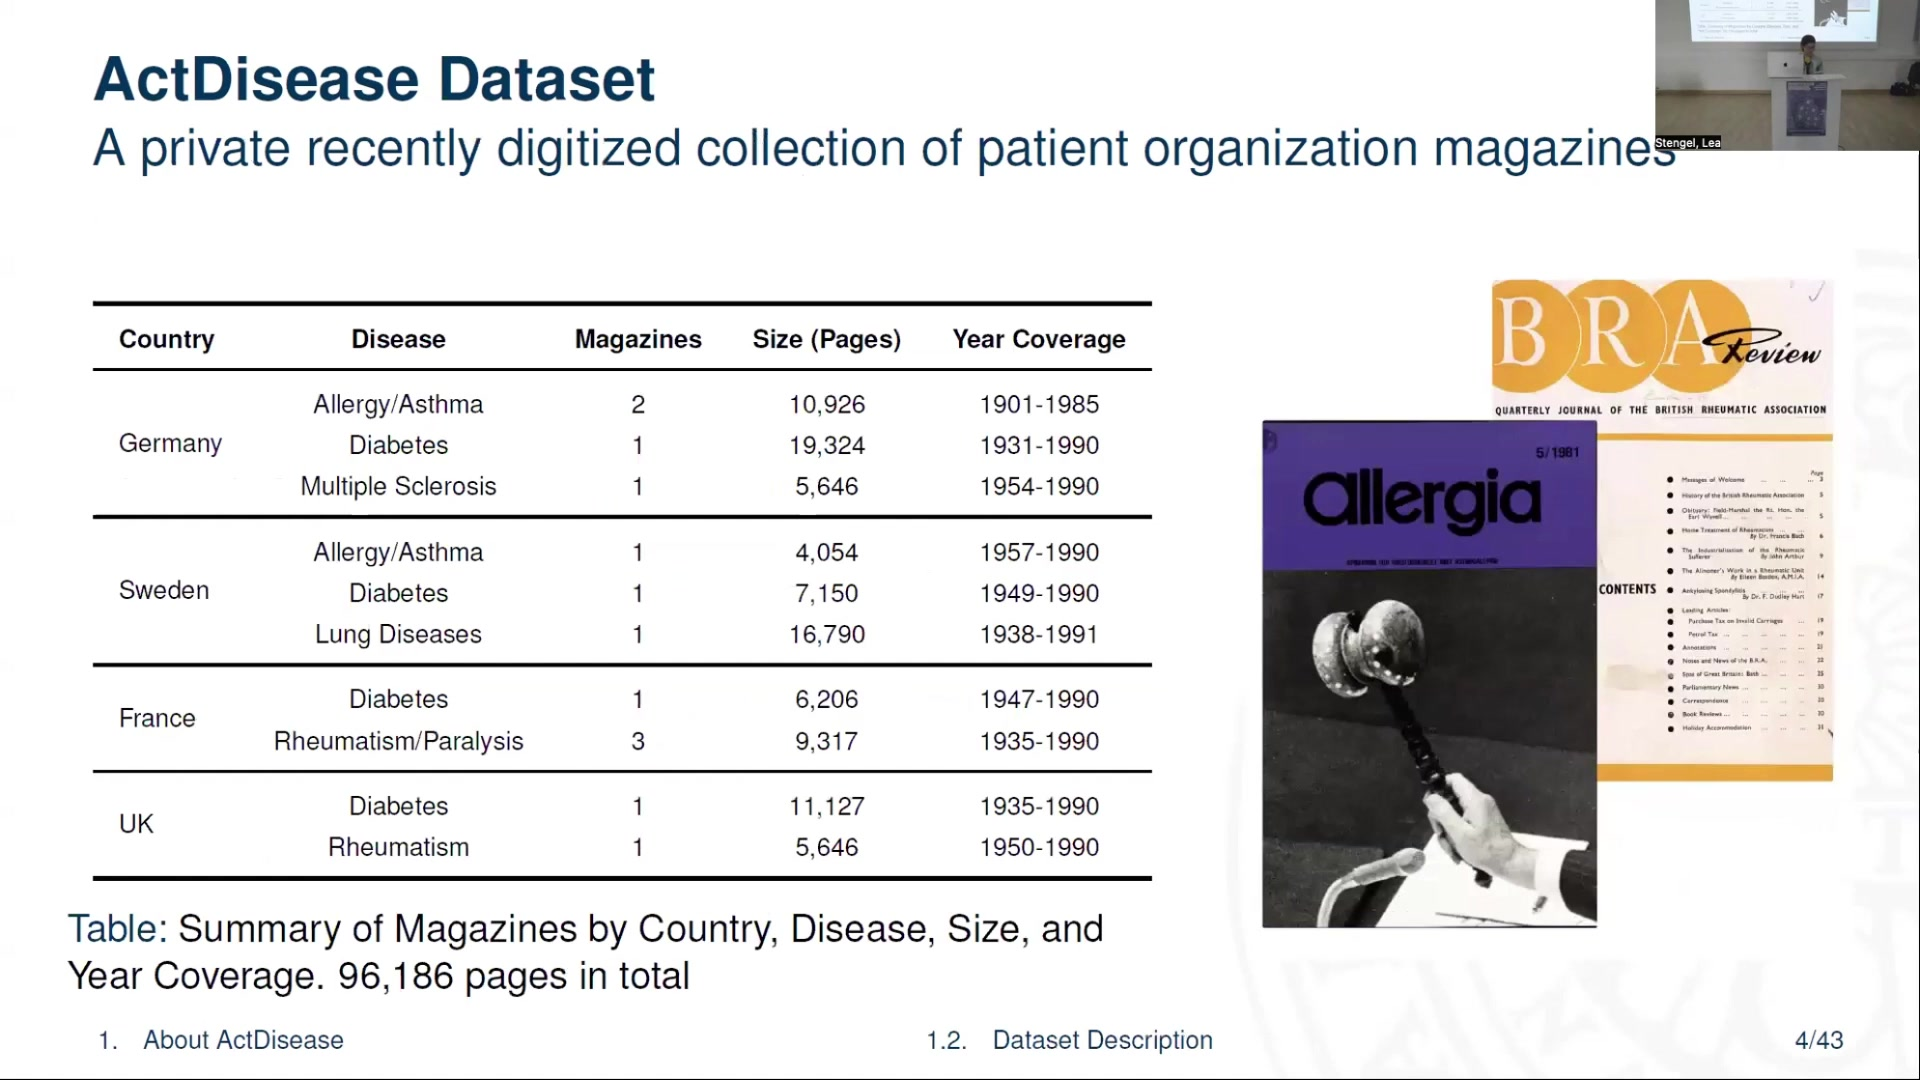
\includegraphics[keepaspectratio]{images/ai-nepi_005_slide_04.jpg}}

}

\caption{Slide detailing the ActDisease Dataset with a table summarising
magazines by country, disease, size, and year coverage, alongside
example magazine covers.}

\end{figure}%

\subsection{Dataset Digitisation
Challenges}\label{dataset-digitisation-challenges}

The digitisation process for the ActDisease dataset primarily involved
Optical Character Recognition (OCR) using ABBYY FineReader Server 14.
Whilst this software performed well on most common layouts and fonts,
several challenges persist. Complex layouts, slanted text, rare fonts,
and varying scan or photograph quality continue to pose difficulties for
OCR accuracy. Consequently, remaining issues include OCR errors,
particularly in German and French texts, and disrupted reading order.
Researchers conducted experiments on post-OCR correction of German texts
using instruction-tuned generative models to address some of these
problems .

Furthermore, OCR errors appear frequently in creative texts, such as
advertisements, humour pages, and poems. A significant challenge arises
from the co-occurrence of different text types within a single
page---for instance, an administrative report might appear alongside an
advertisement and a humour section. This heterogeneity means that
conventional topic models and term counts, which do not account for such
juxtapositions, are likely biased towards the most frequent text type on
a page.

\begin{figure}[H]

{\centering \pandocbounded{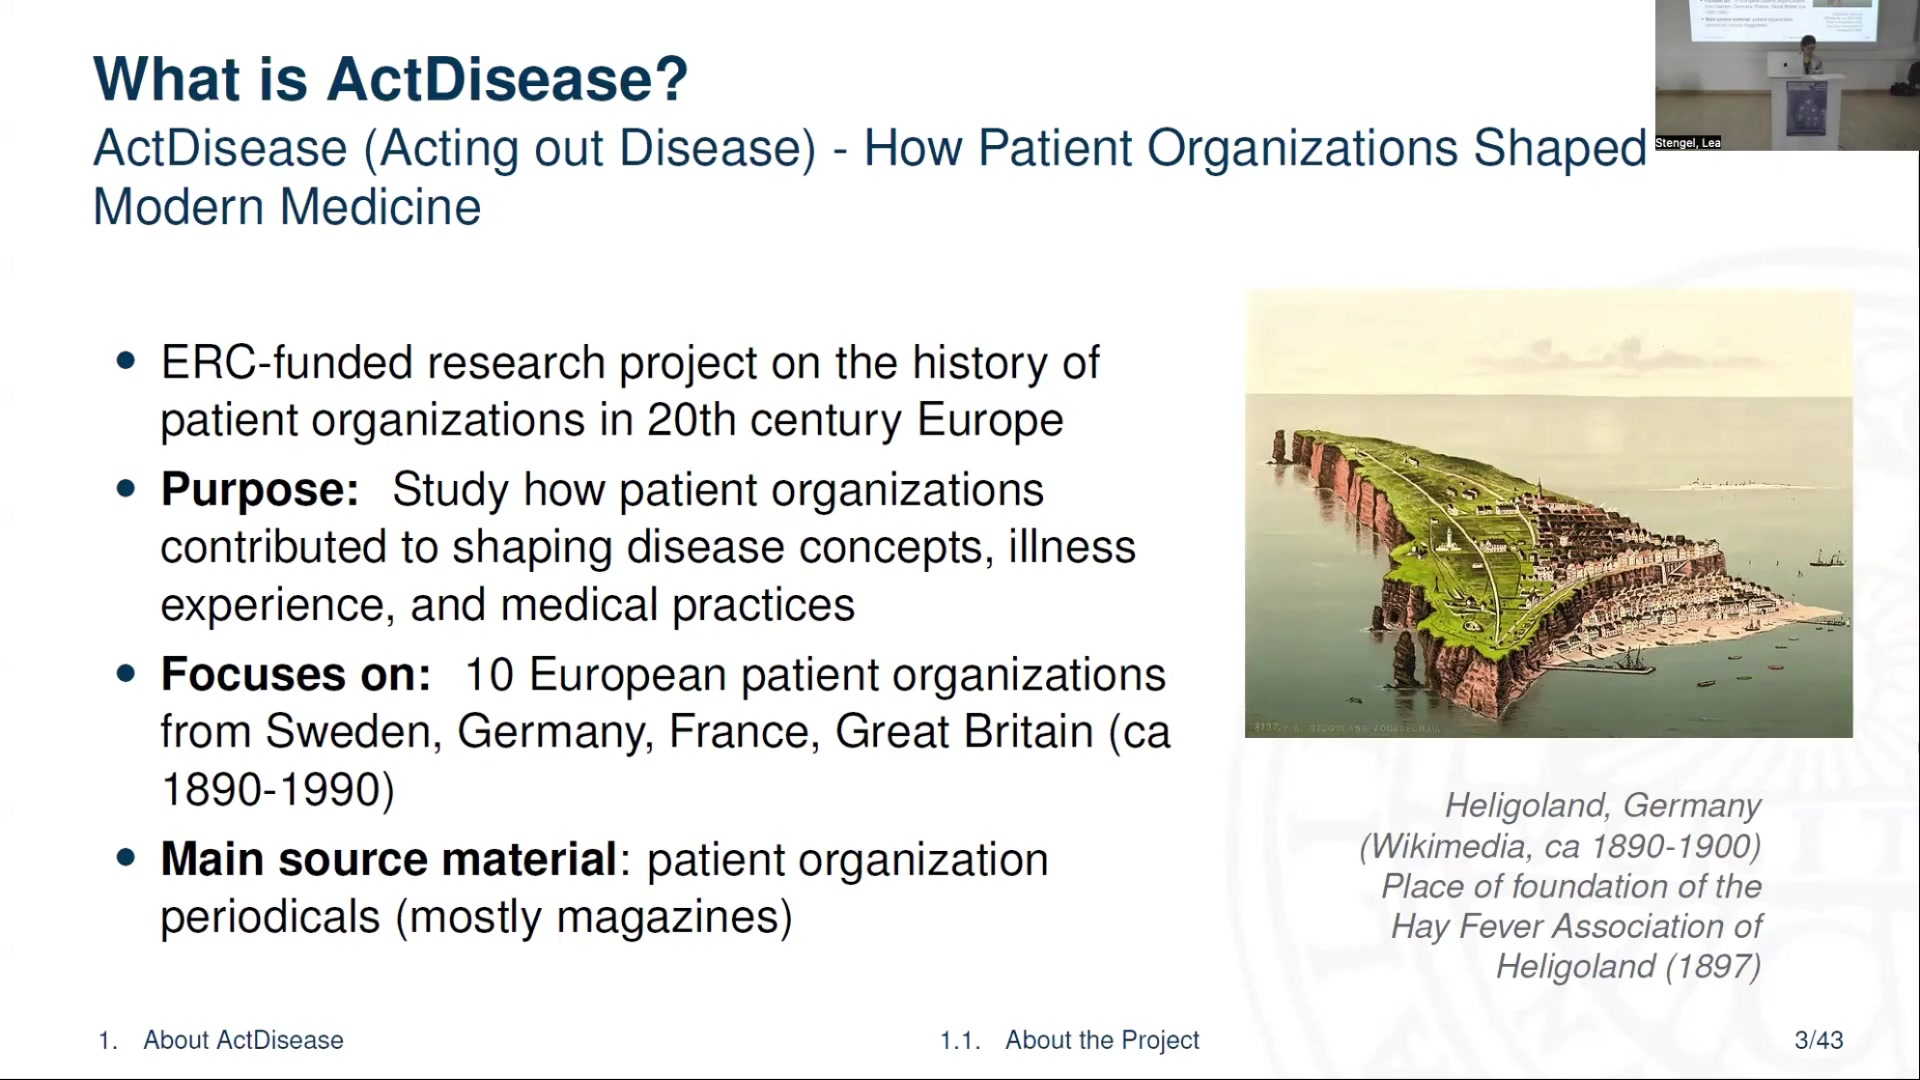
\includegraphics[keepaspectratio]{images/ai-nepi_005_slide_05.jpg}}

}

\caption{Slide outlining digitization challenges, including OCR issues
with complex layouts and creative texts, and showing examples of
historical periodical pages.}

\end{figure}%

\section{Genre Classification
Experiments}\label{genre-classification-experiments}

The inherent diversity of texts within the historical medical
periodicals necessitates a robust method for distinguishing between
them. Genre classification emerges as a pivotal approach to address this
need.

\subsection{Motivation for Genre
Classification}\label{motivation-for-genre-classification}

An examination of the ActDisease materials reveals a wide variety of
text types, which, interestingly, exhibit similarities across all
magazines. Different text types, such as administrative reports,
advertisements, and humour sections, often appear side-by-side on the
same page. This textual diversity poses a challenge for analytical
methods like yearly and decade-based topic models or term counts, as
these methods typically do not account for such internal heterogeneity.

\begin{figure}[H]

{\centering \pandocbounded{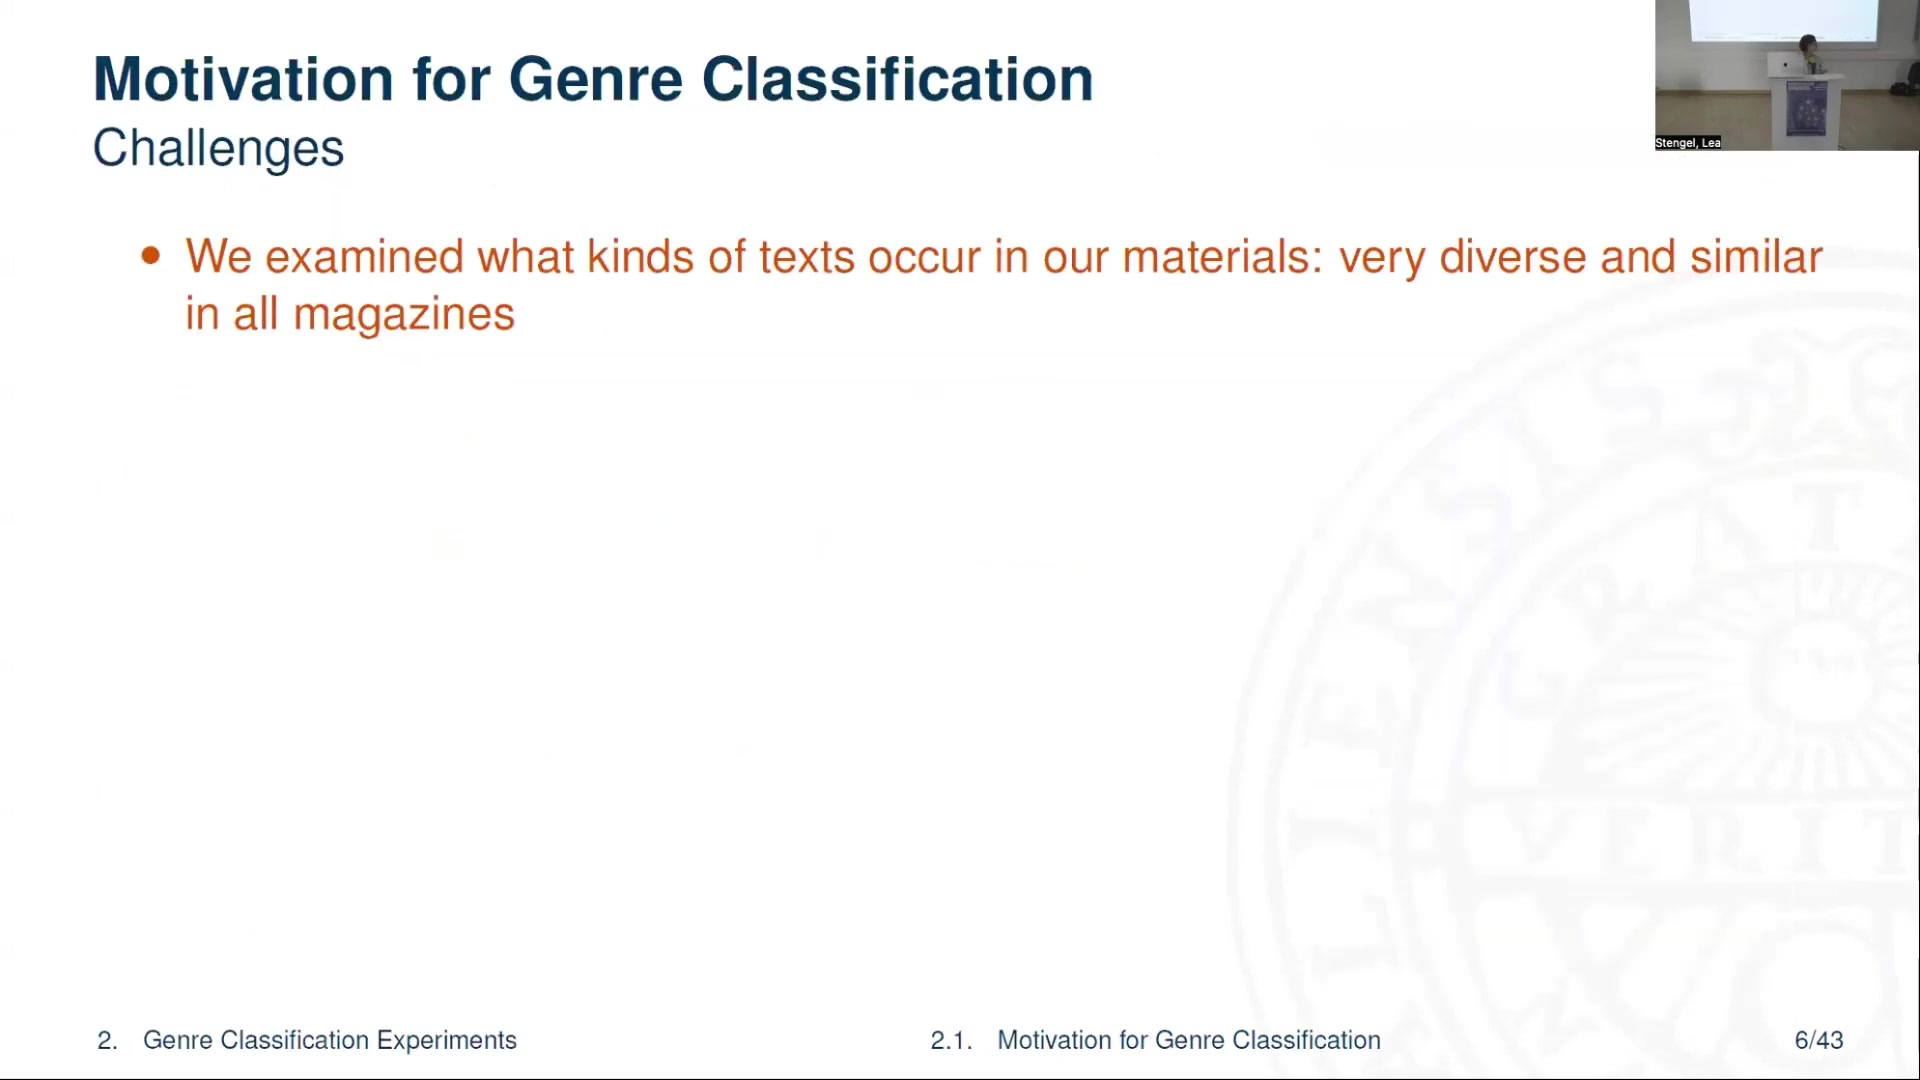
\includegraphics[keepaspectratio]{images/ai-nepi_005_slide_06.jpg}}

}

\caption{Slide highlighting challenges in analysing diverse text types
within historical magazines.}

\end{figure}%

Genre, therefore, presents itself as a useful concept for
differentiating kinds of text. In Language Technology, genre is often
defined as a class of documents sharing a communicative purpose ---a
definition that proves highly applicable here. The ability to classify
genre is crucial for exploring the data from multiple perspectives to
construct historical arguments. Specifically, genre classification
enables the comparative study of communicative strategies across
different countries, diseases, and publications over time . It also
facilitates a more fine-grained analysis of term distributions and topic
models within distinct genre groups.

\begin{figure}[H]

{\centering \pandocbounded{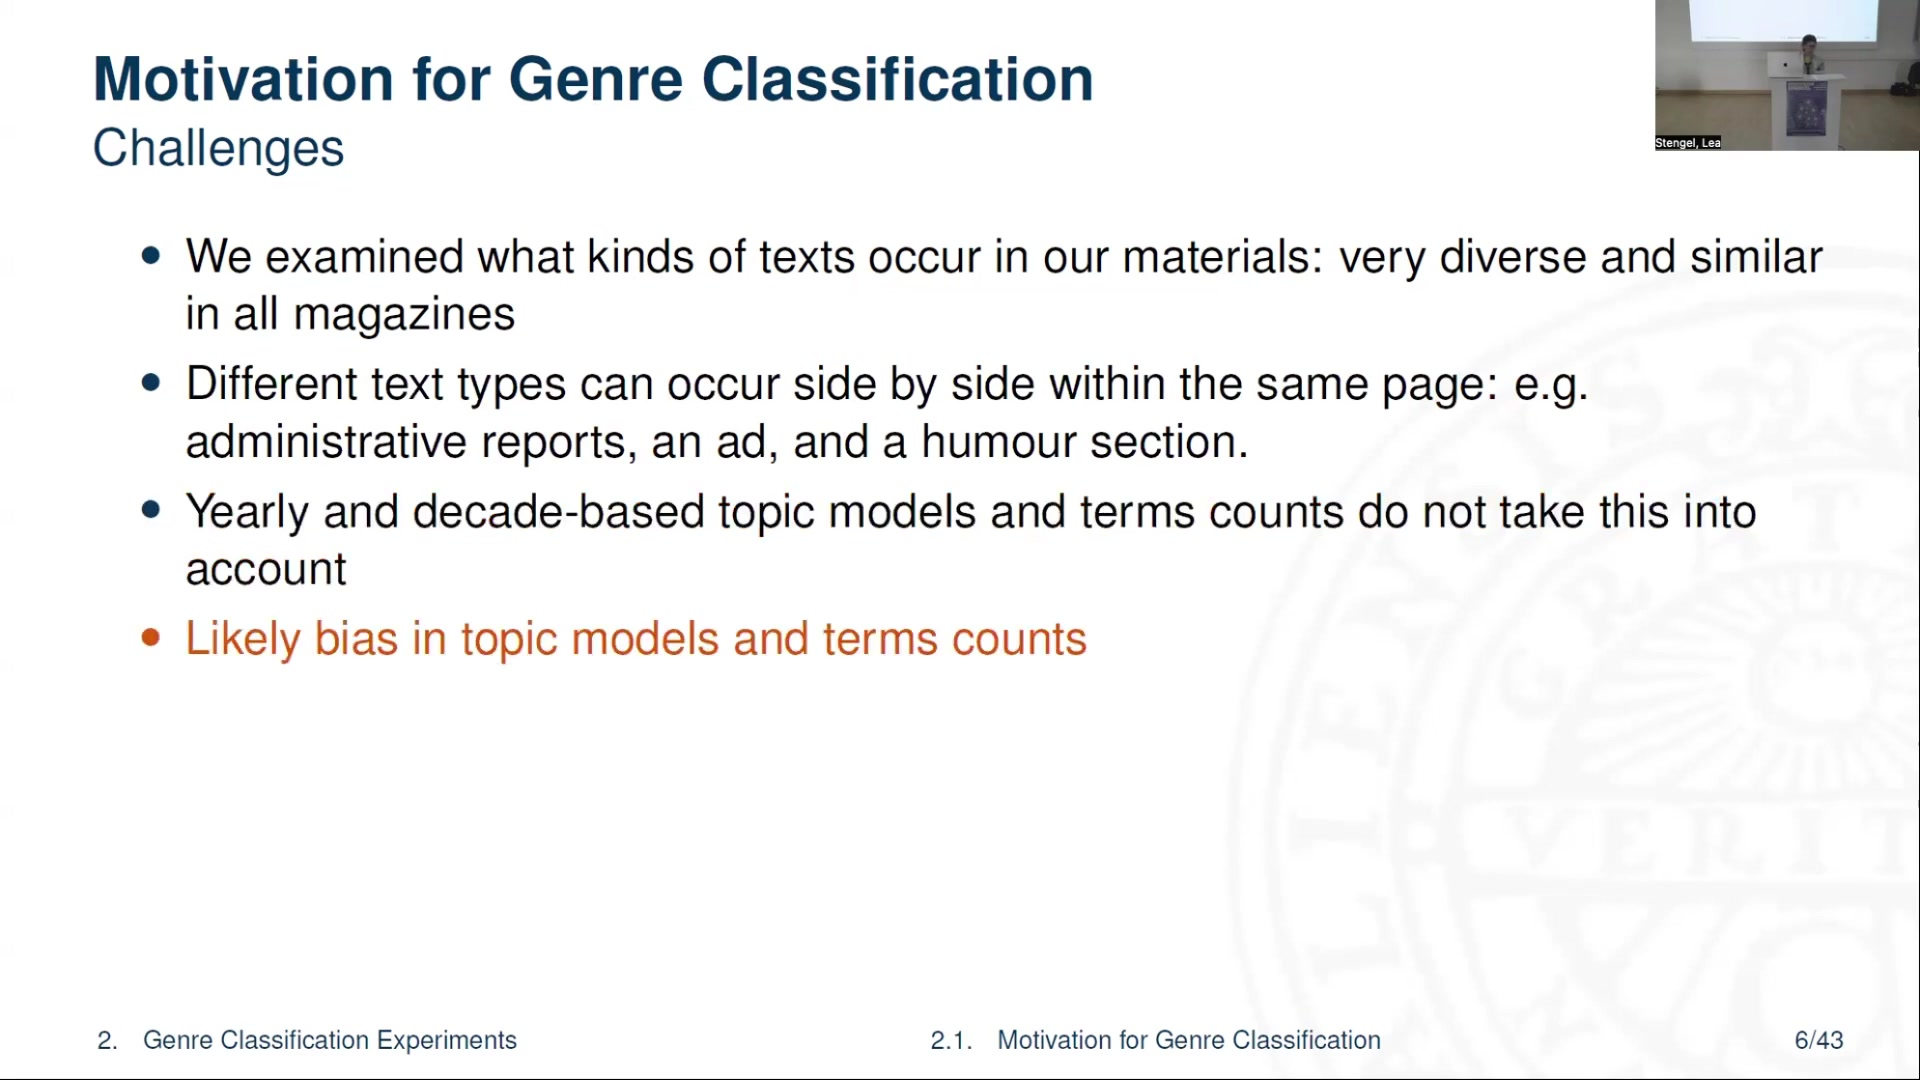
\includegraphics[keepaspectratio]{images/ai-nepi_005_slide_07.jpg}}

}

\caption{Slide explaining why genre is a useful concept for
classification and its benefits for historical analysis.}

\end{figure}%

The ActDisease data showcases a rich tapestry of genres. Examples
include poetry, academic reports (such as studies on the pancreas),
legal documents (like deeds of covenant), and advertisements (for
instance, for chocolate aimed at diabetics). Instructive messages,
including recipes or medical advice, feature prominently, alongside
patient organisation reports detailing meetings and activities.
Narratives about patients' lives also constitute a significant portion
of the content.

\begin{figure}[H]

{\centering \pandocbounded{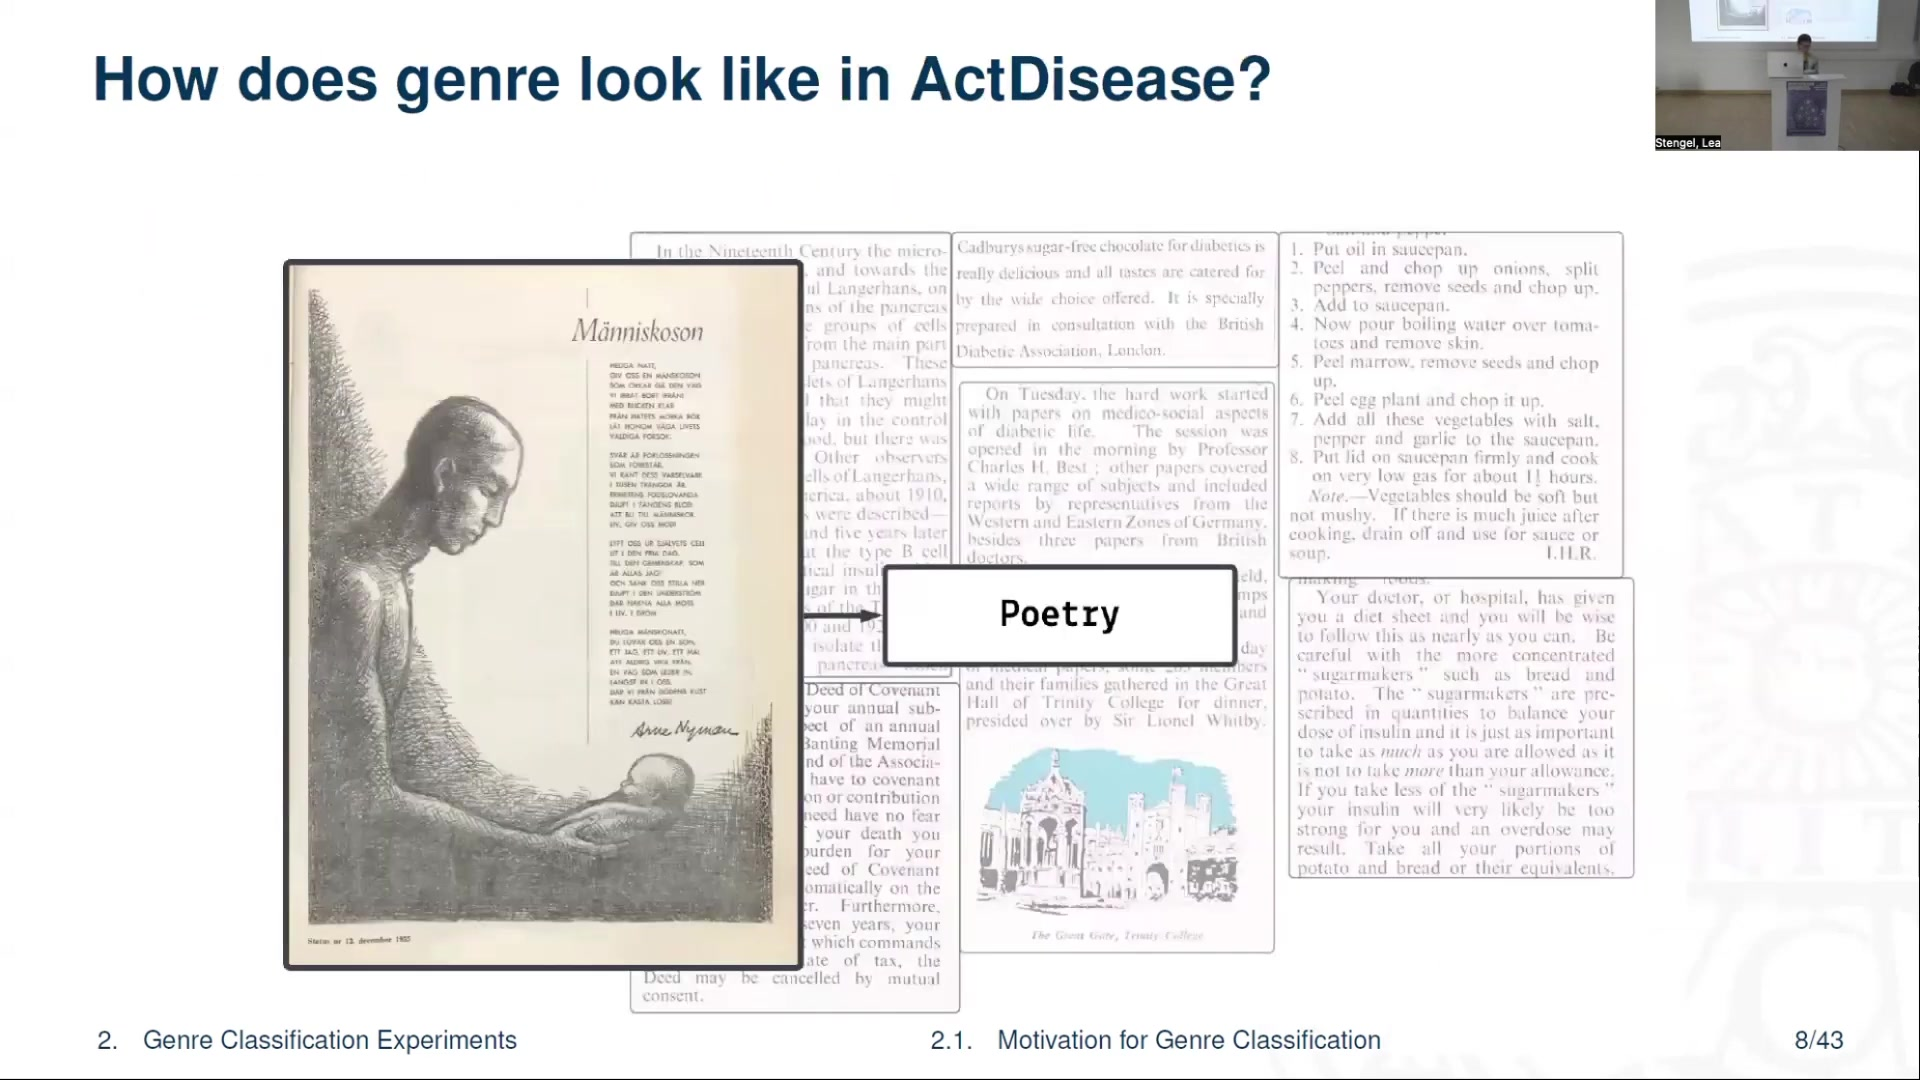
\includegraphics[keepaspectratio]{images/ai-nepi_005_slide_09.jpg}}

}

\caption{Slide illustrating the variety of genres found in the
ActDisease dataset, such as patient experiences, advertisements, and
instructive texts.}

\end{figure}%

\subsection{Zero-Shot and Few-Shot
Classification}\label{zero-shot-and-few-shot-classification}

Given the scarcity of annotated data within the ActDisease project,
researchers explored both zero-shot and few-shot learning approaches for
genre classification . For zero-shot learning, key research questions
focused on whether genre labels from publicly available datasets could
be efficiently mapped to the project's custom labels and how performance
would vary across different datasets and models. For few-shot learning,
the investigation centred on how performance changes with varying
training set sizes across models and whether prior fine-tuning on the
full dataset could substantially enhance performance.

\begin{figure}[H]

{\centering \pandocbounded{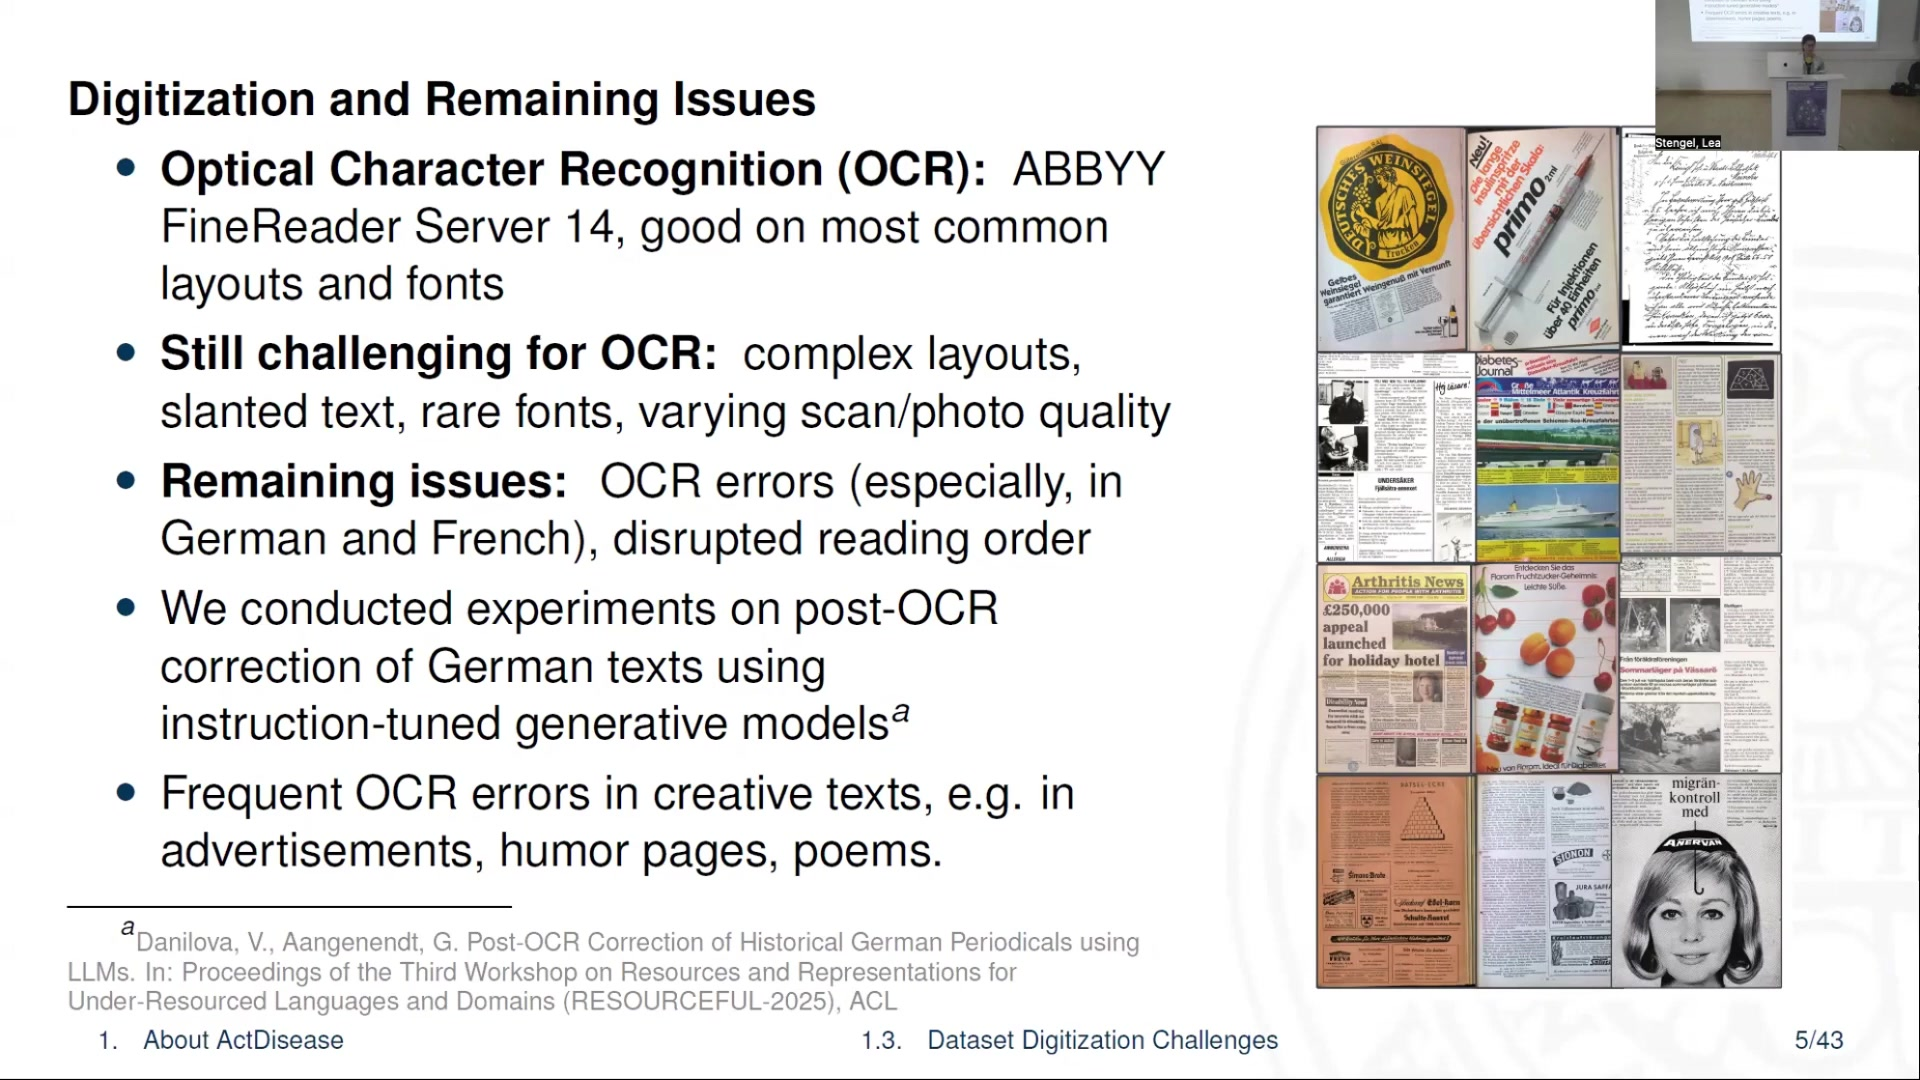
\includegraphics[keepaspectratio]{images/ai-nepi_005_slide_10.jpg}}

}

\caption{Slide outlining research questions for zero-shot and few-shot
learning due to limited annotated data.}

\end{figure}%

\subsubsection{Genre Definition and
Annotation}\label{genre-definition-and-annotation}

The project team, under the supervision of the main historian, defined
the genre labels. The aim was to create labels that are useful for
separating content within the ActDisease materials and sufficiently
general for potential application to similar datasets. The defined
genres include:

\begin{itemize}
\tightlist
\item
  Academic: Research-based reports or explanations of scientific ideas
  (e.g., research article, report).
\item
  Administrative: Documents on organisational activities (e.g., meeting
  minutes, reports, announcements).
\item
  Advertisement: Promotes products or services for commercial purposes.
\item
  Guide: Provides step-by-step instructions (e.g., health tips, legal
  advice, recipes).
\item
  Fiction: Entertains and emotionally engages (e.g., stories, poems,
  humour, myths).
\item
  Legal: Explains legal terms and conditions (e.g., contracts, rules,
  amendments).
\item
  News: Reports recent events and developments.
\item
  Nonfiction Prose: Narrates real events or describes
  cultural/historical topics (e.g., memoir, essay, documentary).
\item
  QA (Question \& Answer): Structured as questions with expert answers,
  typically from periodical sections.
\end{itemize}

\begin{figure}[H]

{\centering \pandocbounded{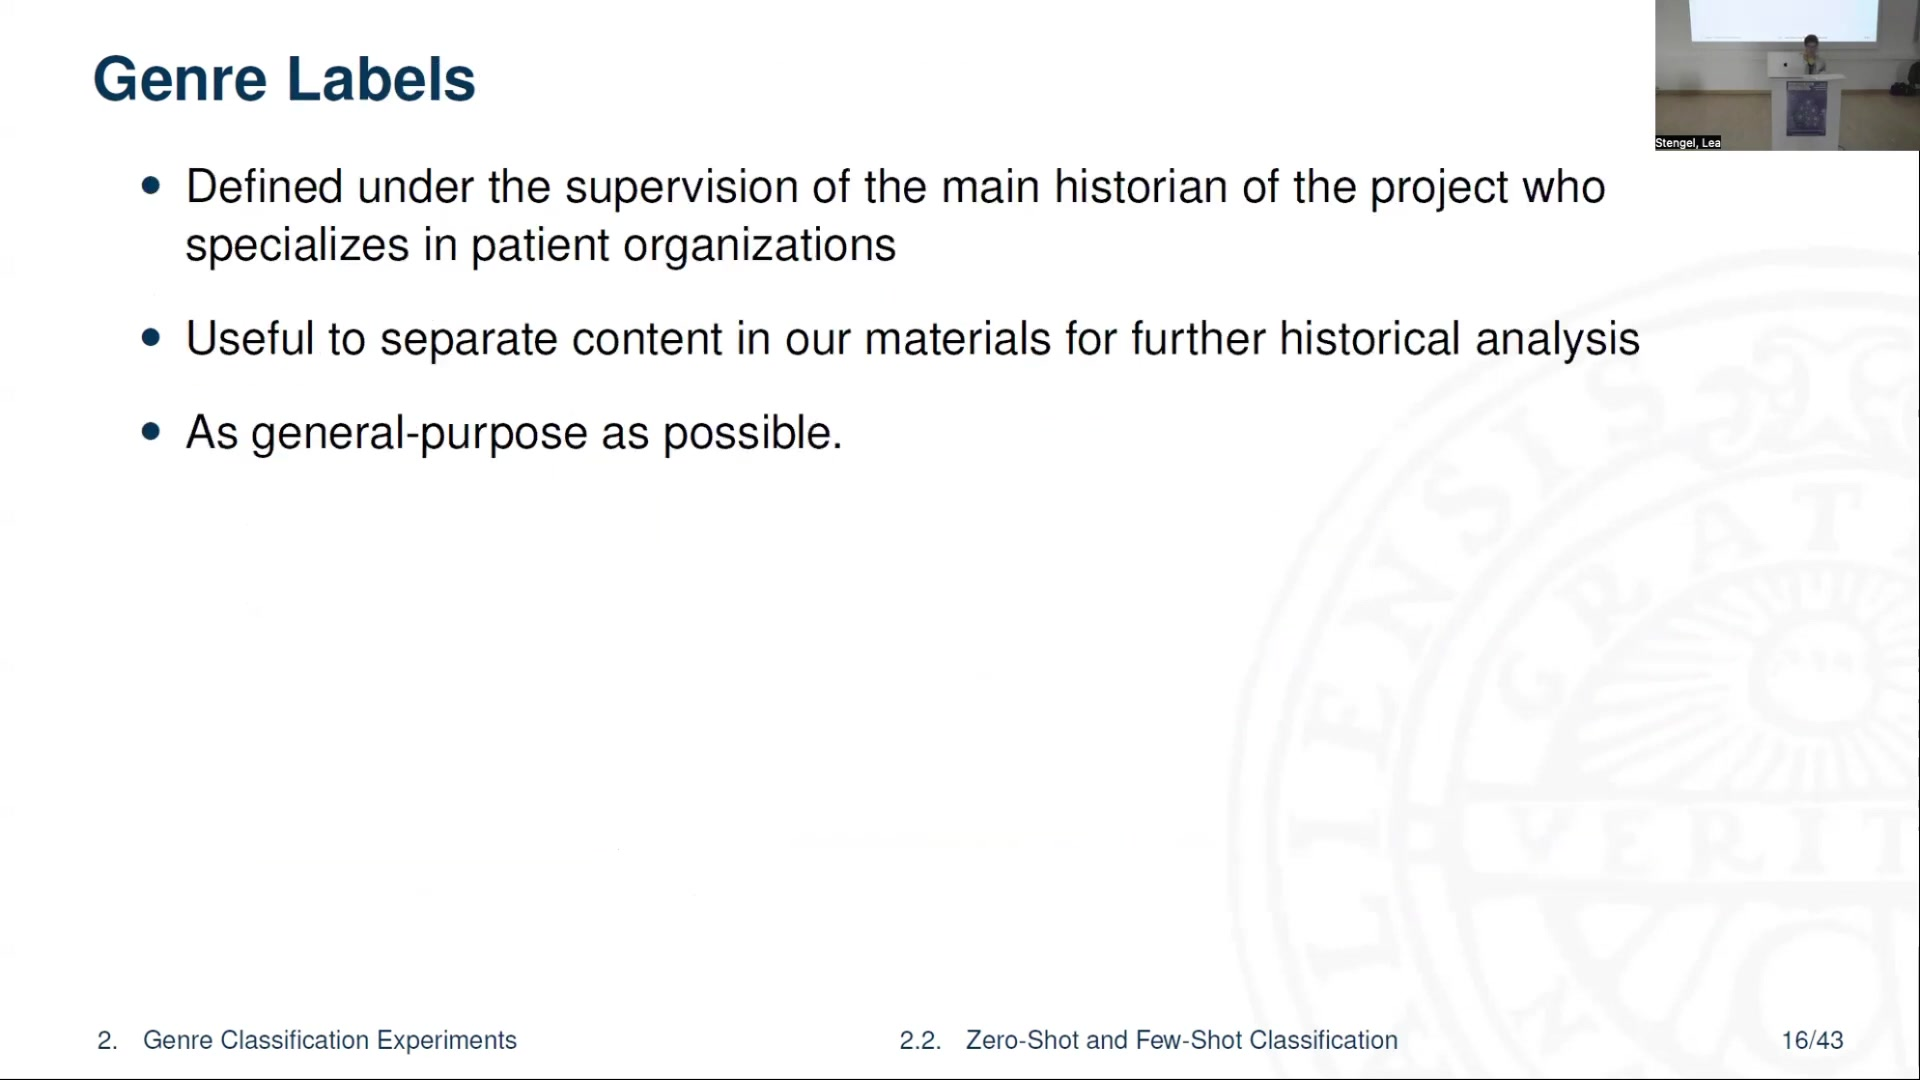
\includegraphics[keepaspectratio]{images/ai-nepi_005_slide_12.jpg}}

}

\caption{Slide presenting a table of genres and their definitions used
in the ActDisease project.}

\end{figure}%

Researchers selected the paragraph as the annotation unit, merging
paragraphs from the ABBYY FineReader output based on font patterns
(type, size, bold, italic) within a page. Annotators sampled from two
periodicals: the Swedish ``Diabetes'' and the German ``Diabetiker
Journal'', specifically focusing on the first and mid-year issues for
each year. A team of four historians and two computational linguists,
all either native or proficient in Swedish and German, performed the
annotation. Each paragraph received two annotations, achieving an
average inter-annotator agreement of 0.95 Krippendorff's alpha,
indicating a high level of consistency. Annotators used a structured
file format, assigning hard genre labels to each paragraph.

\pandocbounded{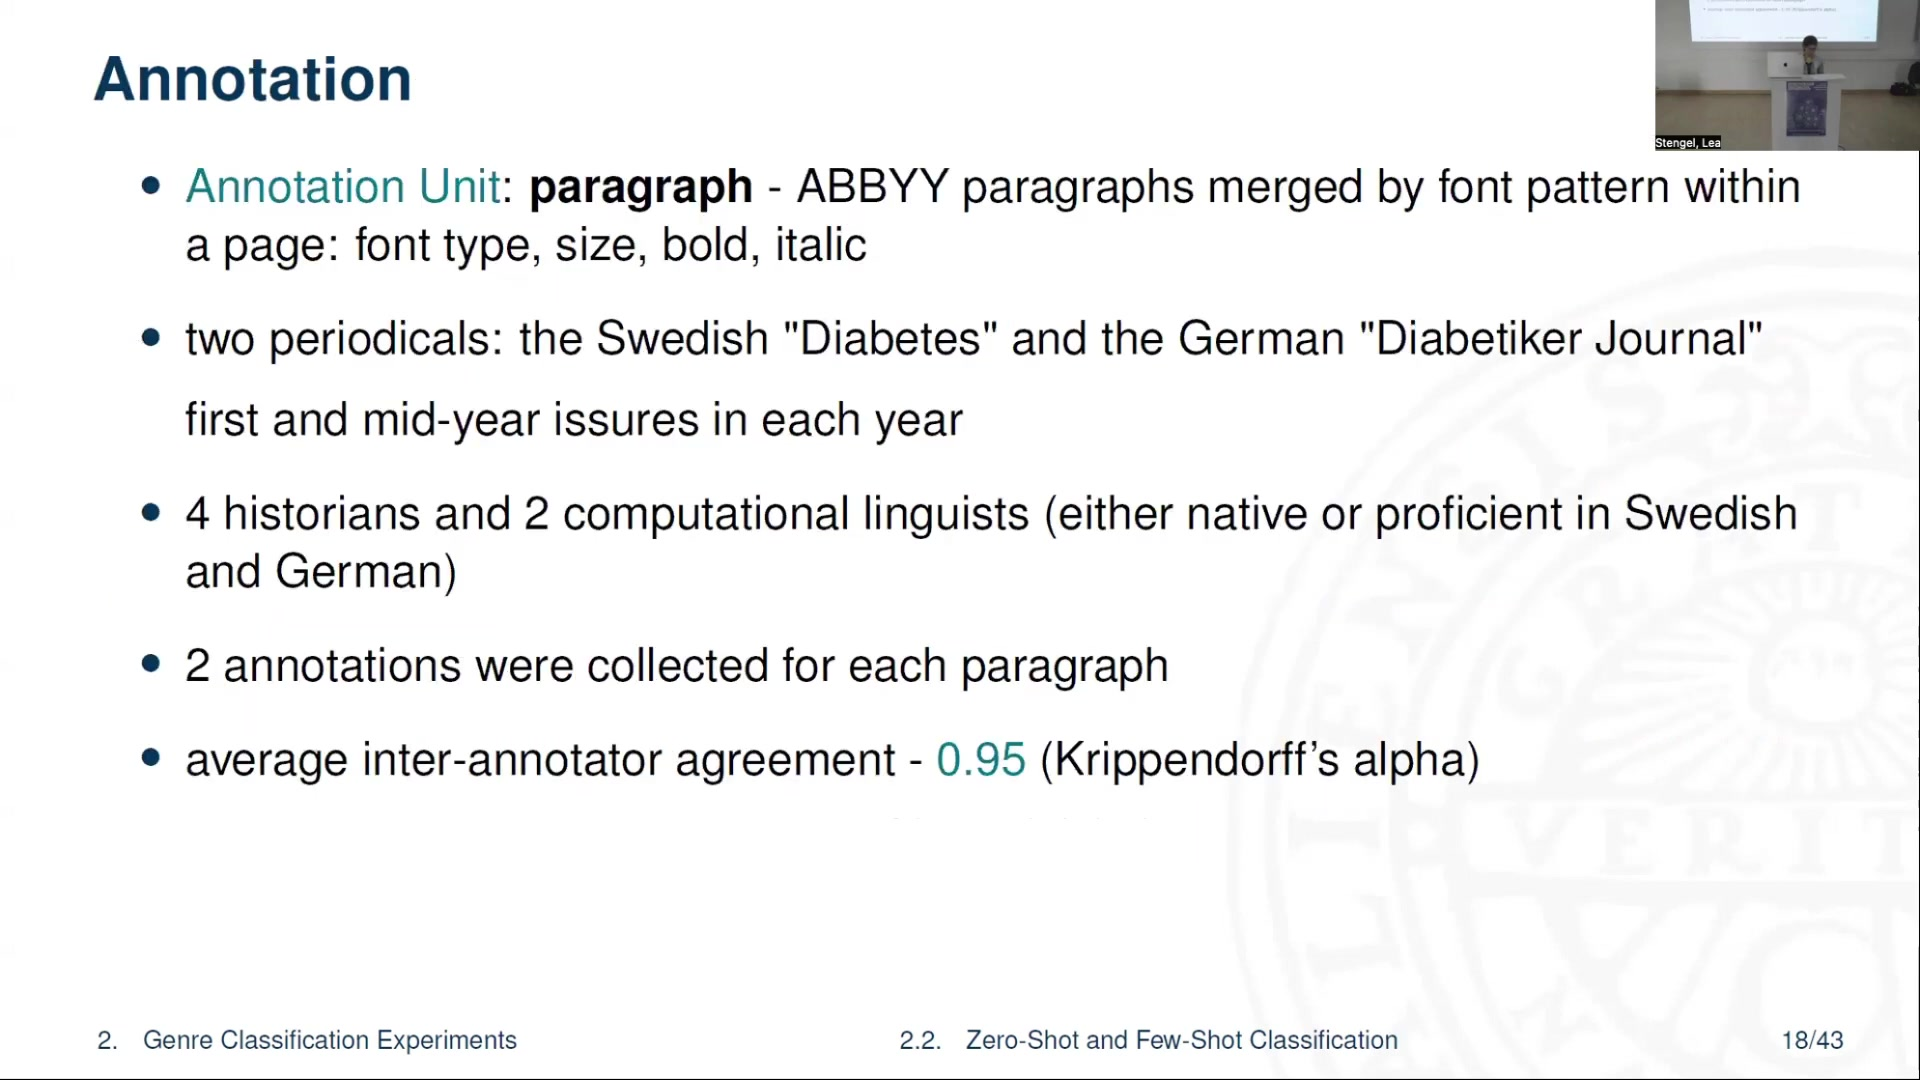
\includegraphics[keepaspectratio]{images/ai-nepi_005_slide_14.jpg}}
\pandocbounded{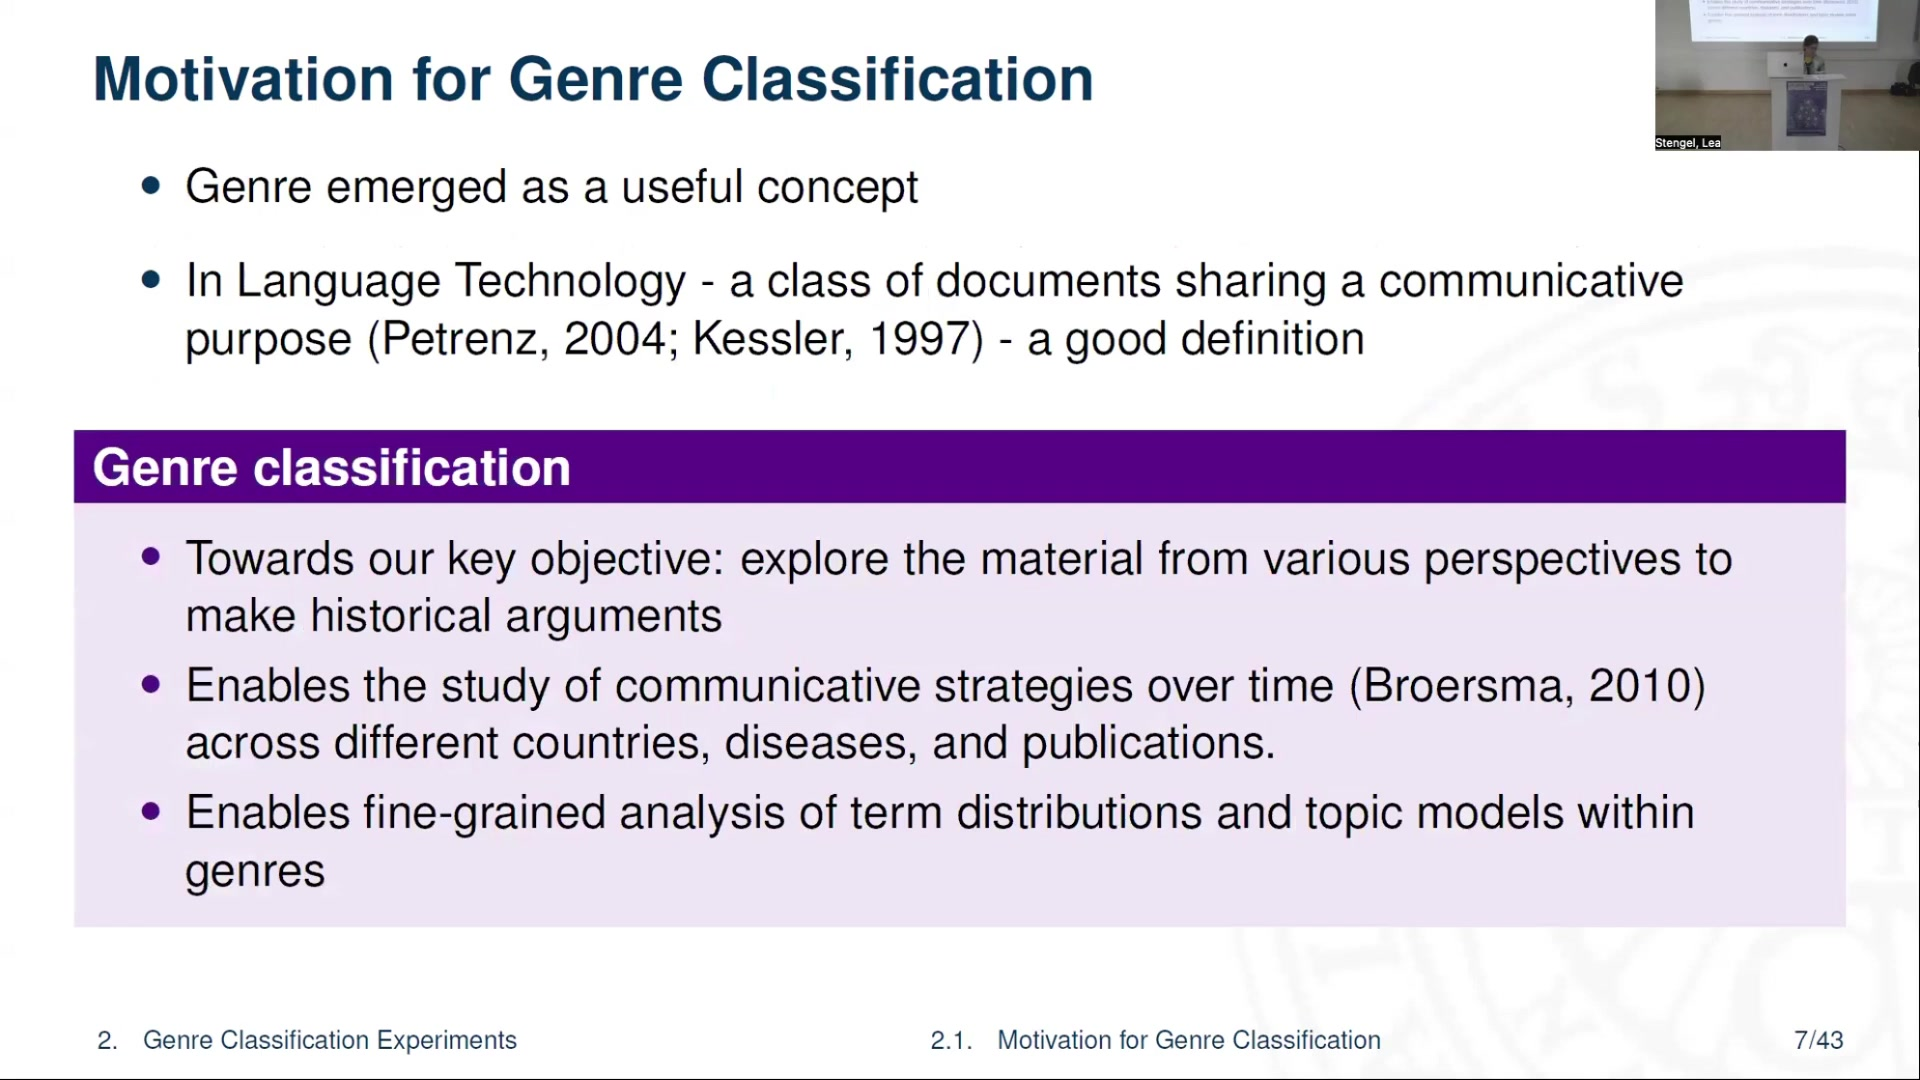
\includegraphics[keepaspectratio]{images/ai-nepi_005_slide_15.jpg}}

\subsubsection{Data Splits and
Distribution}\label{data-splits-and-distribution}

For the experiments, researchers first split the annotated data into
training and held-out sets, with the held-out set comprising
approximately 30\% of the data. For few-shot experiments, they further
divided the held-out set equally and balanced it by label. Researchers
excluded the `Legal' and `News' genres from these few-shot experiments
due to insufficient training data. Researchers utilised the entire test
set for zero-shot experiments. The distribution of genres across
languages (German and Swedish) in the training and held-out samples
reveals some imbalances. Notably, there is a strong imbalance in
`Advertisement' and `Nonfiction Prose' across the two languages.

\begin{figure}[H]

{\centering \pandocbounded{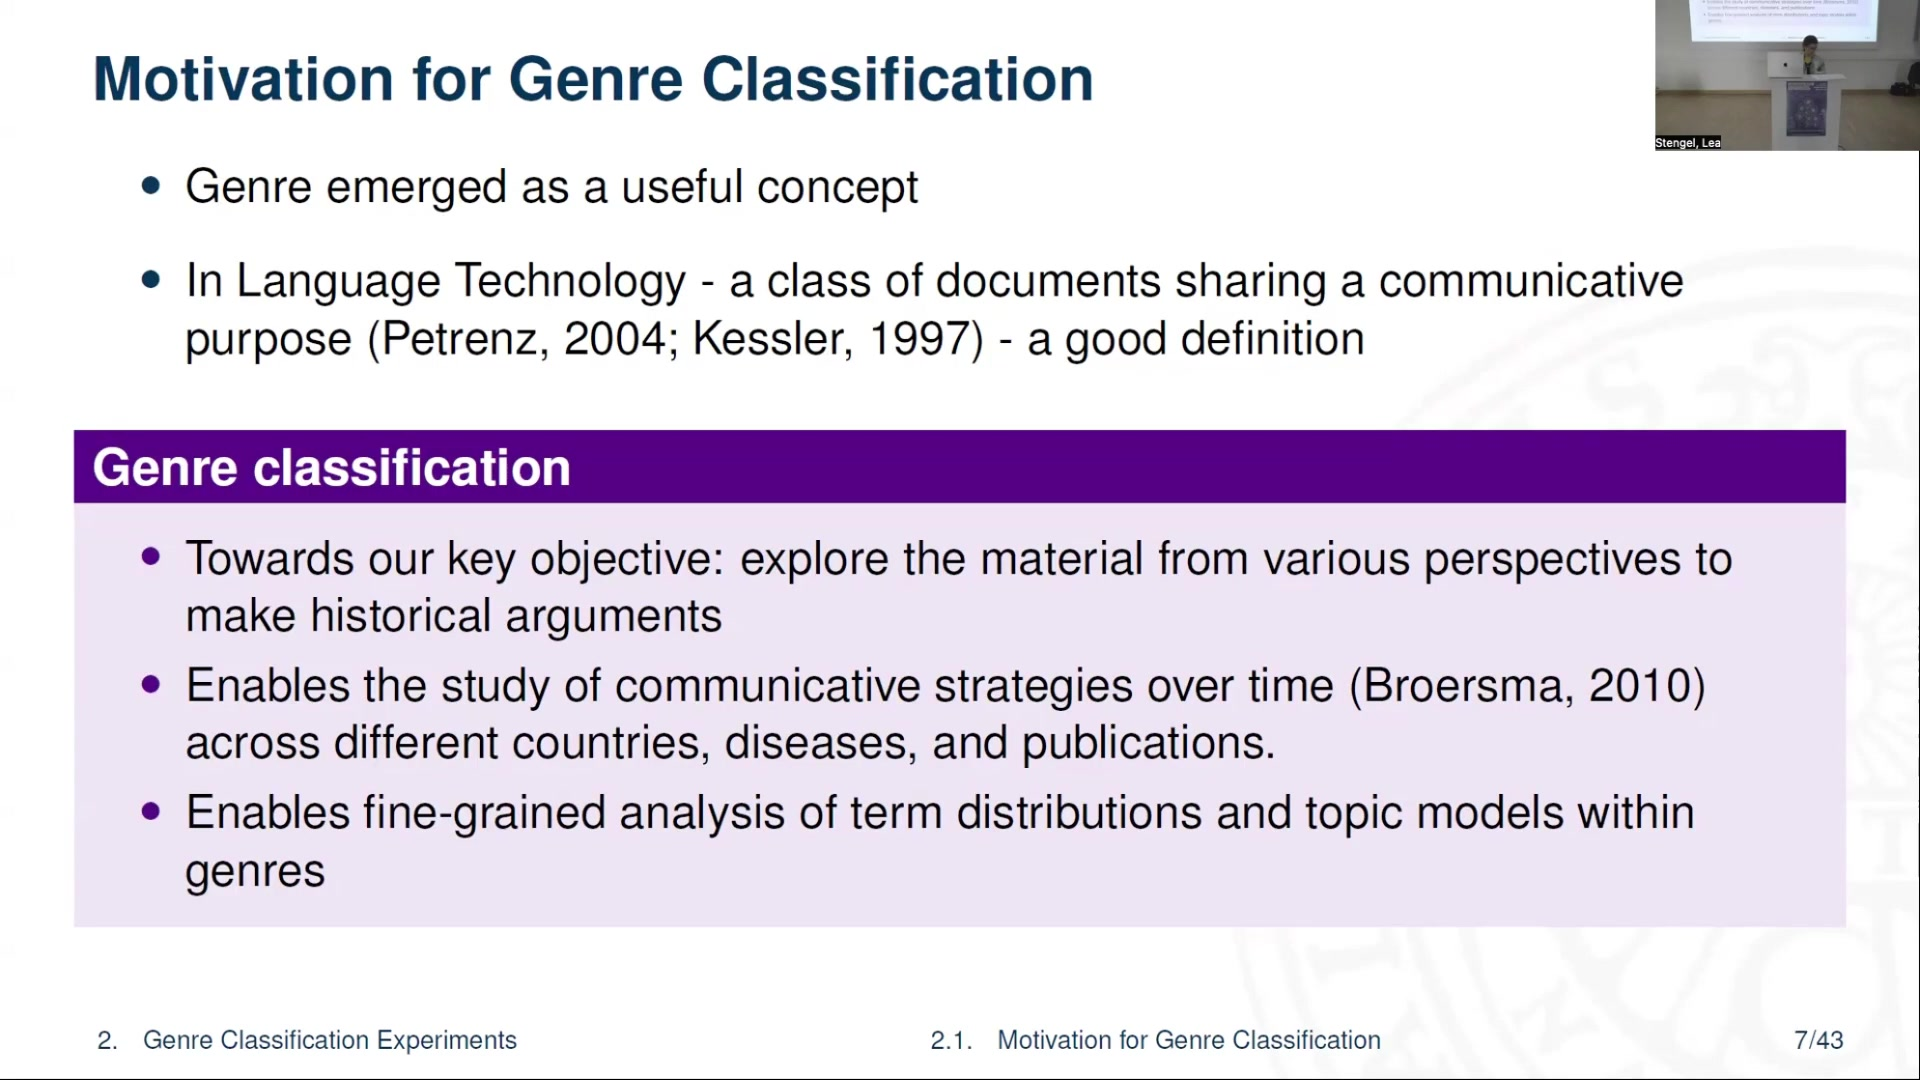
\includegraphics[keepaspectratio]{images/ai-nepi_005_slide_16.jpg}}

}

\caption{Slide presenting bar charts of genre distribution in the
ActDisease training and held-out samples for German and Swedish
languages.}

\end{figure}%

\subsubsection{External Datasets and Genre Mapping for Zero-Shot
Learning}\label{external-datasets-and-genre-mapping-for-zero-shot-learning}

To facilitate zero-shot experiments, researchers incorporated external
datasets. These included modern datasets from previous work on automatic
web genre classification: the Corpus of Online Registers of English
(CORE) and the Functional Text Dimensions (FTD) dataset, both annotated
at the document level. Additionally, they used a sample from Universal
Dependencies (UDM) Treebanks, which contains sentence-level annotations
in multiple languages.

Two annotators independently performed the genre mapping from these
external datasets to the ActDisease categories. For the final mapping,
researchers selected only assignments with full agreement. This process
revealed that for some ActDisease genres, no directly suitable labels
existed in the available external datasets. The pipeline for creating
training data involved this mapping, followed by preprocessing,
chunking, and sampling in several configurations based on language
family and label levels (ActDisease original vs.~external dataset
original).

\begin{figure}[H]

{\centering \pandocbounded{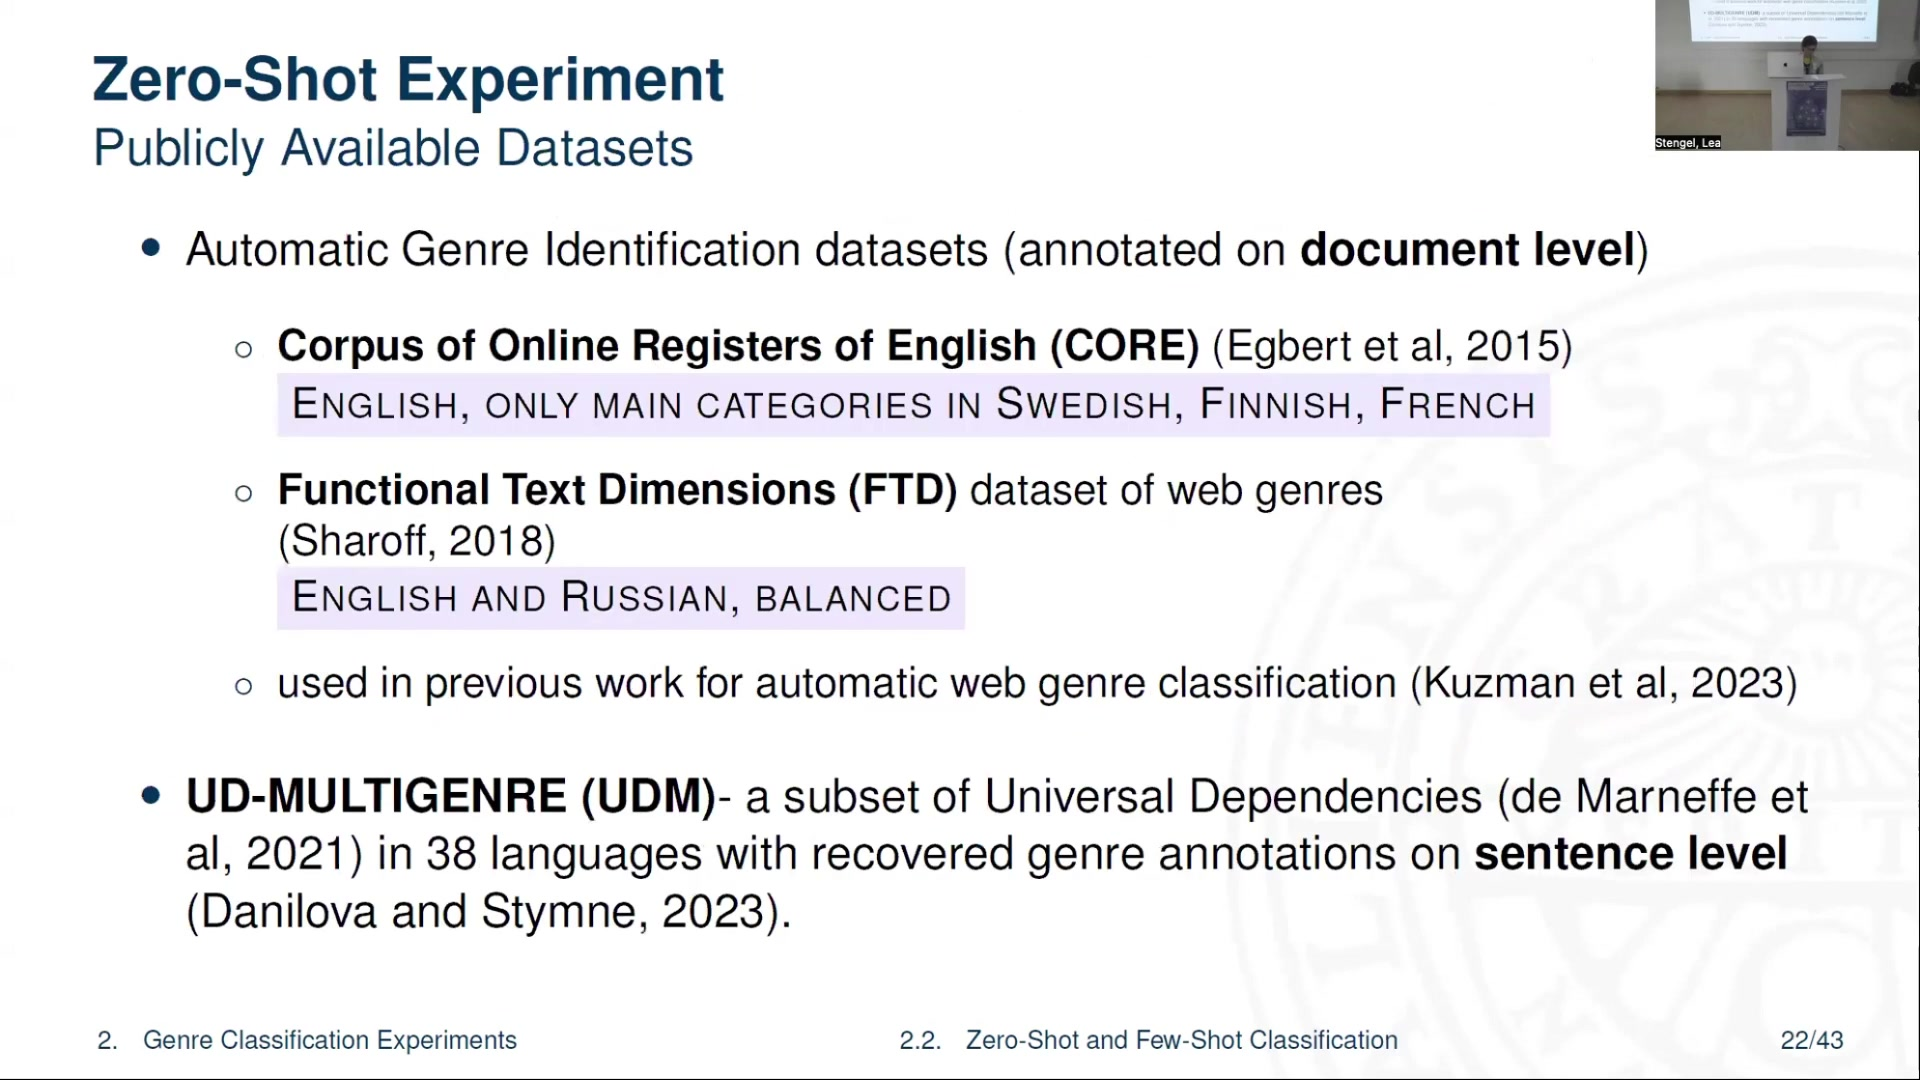
\includegraphics[keepaspectratio]{images/ai-nepi_005_slide_18.jpg}}

}

\caption{Slide showing a table mapping ActDisease genre categories to
those in CORE, UDM, and FTD datasets.}

\end{figure}%

\subsubsection{Models Employed}\label{models-employed}

Researchers selected multilingual encoders for these experiments, models
that have demonstrated success in previous automatic genre
classification tasks. The chosen models were:

\begin{itemize}
\tightlist
\item
  XLM-RoBERTa
\item
  mBERT (multilingual BERT)
\item
  historical mBERT (hmBERT)
\end{itemize}

BERT-like models have seen extensive use in prior work on web register
and genre classification . XLM-RoBERTa is recognised as a
state-of-the-art web genre classifier . The inclusion of hmBERT was
particularly pertinent as it is pretrained on a large corpus of
multilingual historical newspapers, encompassing the languages in the
ActDisease dataset. mBERT was included for comparison with hmBERT, as
direct comparison with XLM-RoBERTa is not straightforward. Fine-tuning
these models on all configurations of the training data (derived from
FTD, CORE, UDM, and a merged set) yielded a total of 48 fine-tuned
models. Researchers typically average subsequent metrics across these
configurations.

\pandocbounded{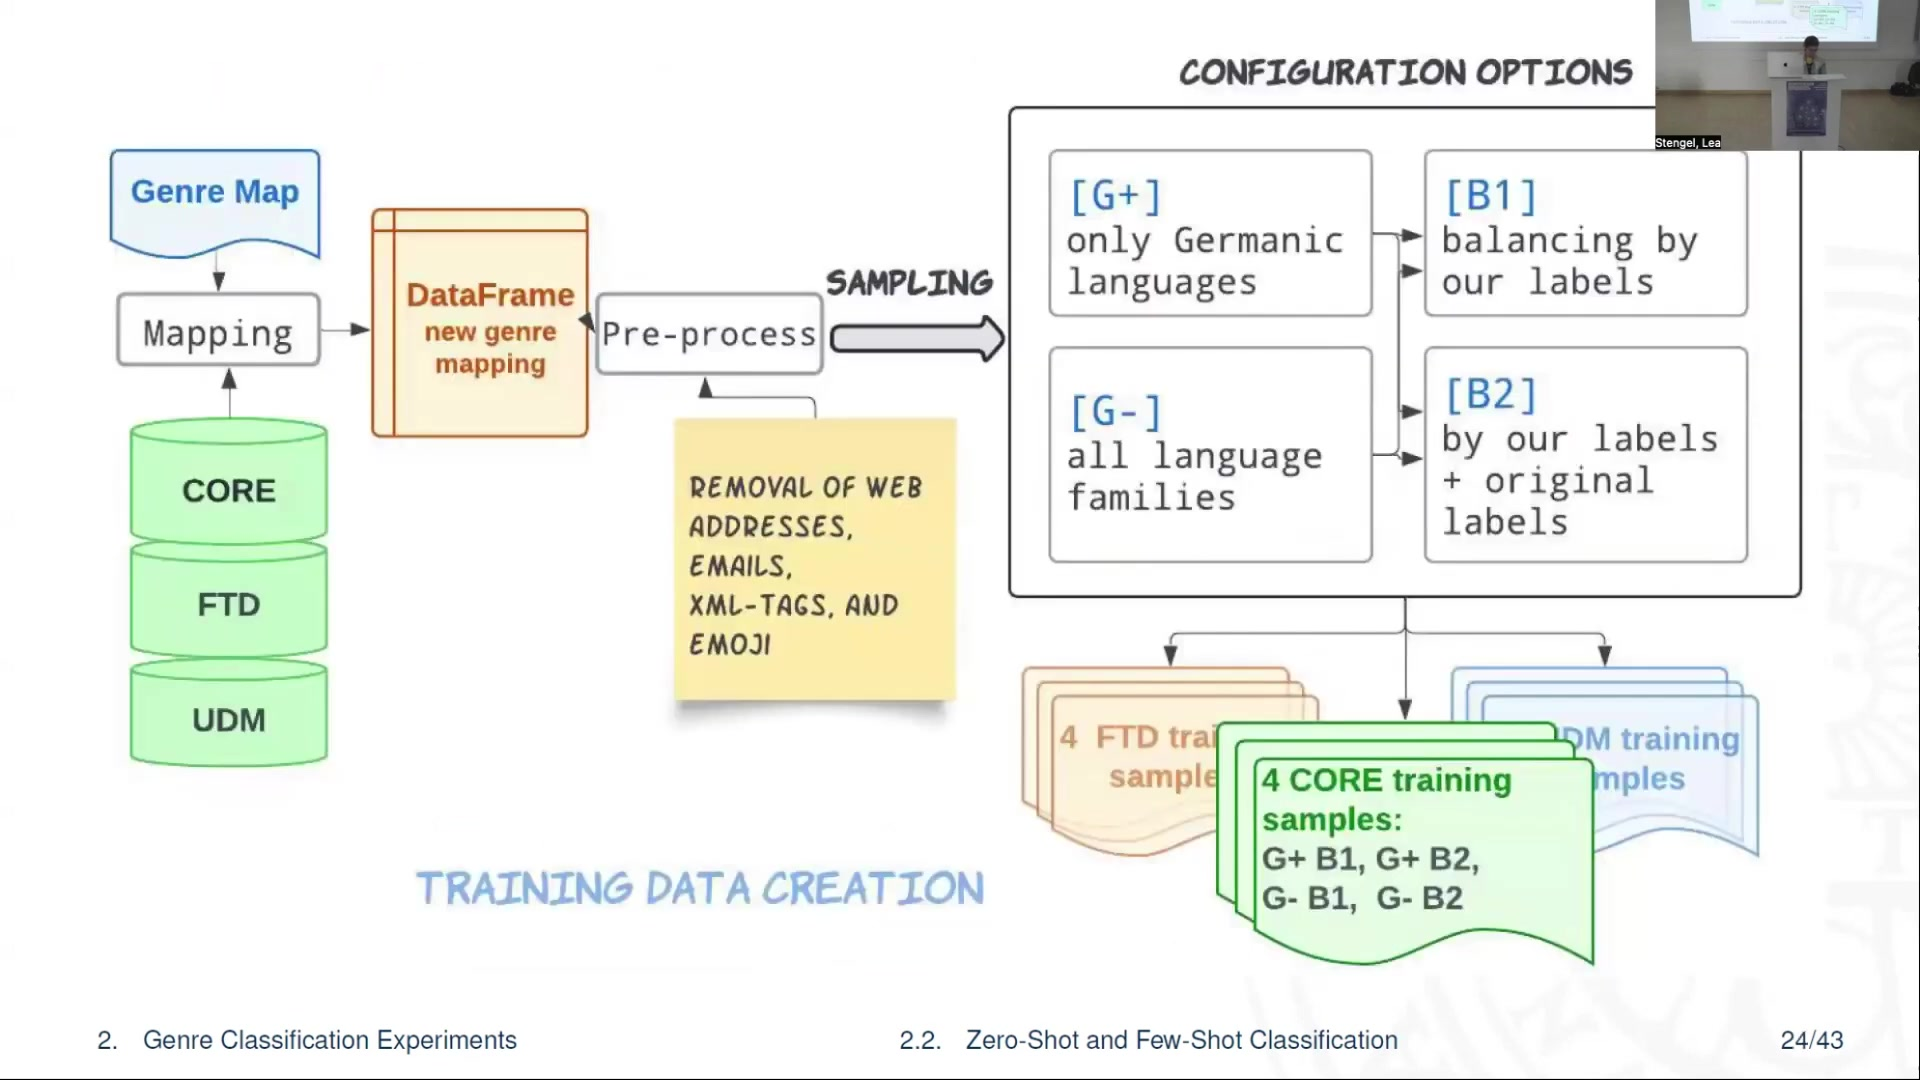
\includegraphics[keepaspectratio]{images/ai-nepi_005_slide_20.jpg}}
\pandocbounded{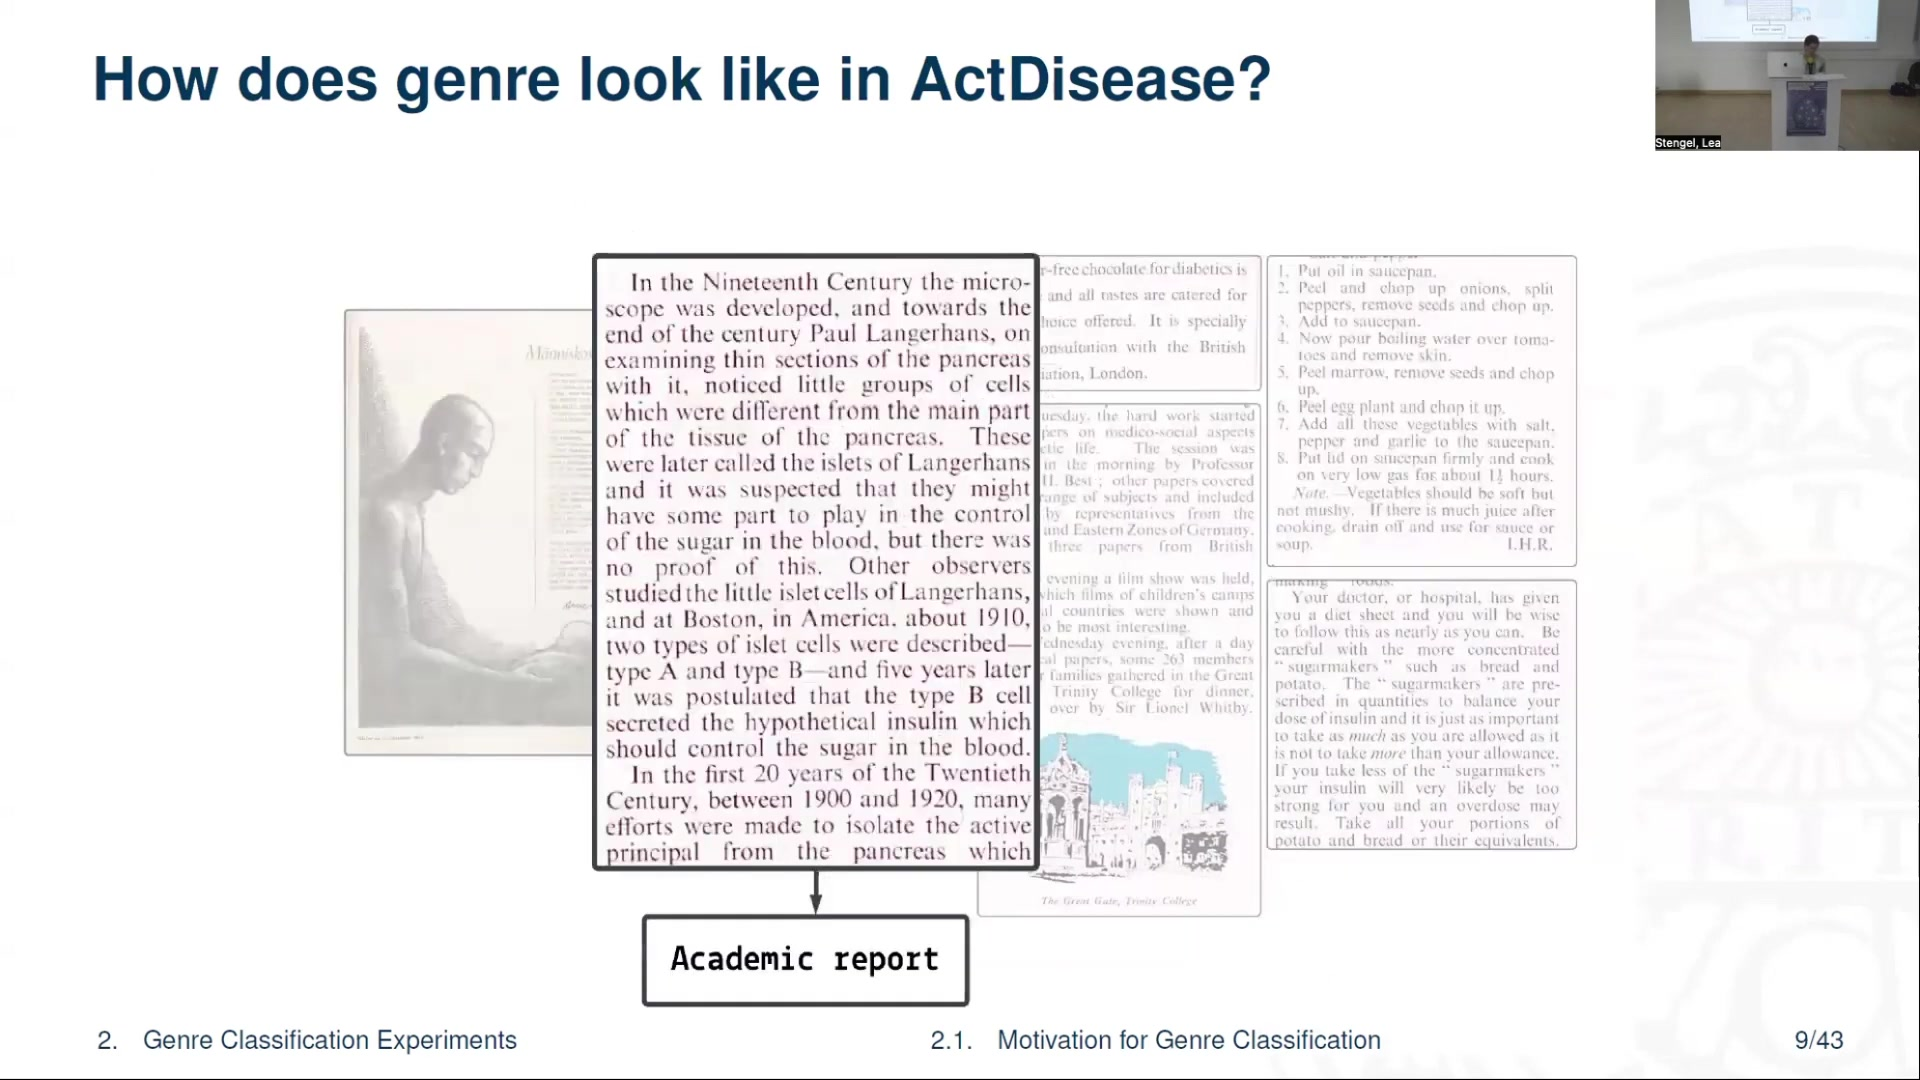
\includegraphics[keepaspectratio]{images/ai-nepi_005_slide_21.jpg}}

\subsubsection{Zero-Shot Learning
Evaluation}\label{zero-shot-learning-evaluation}

In evaluating zero-shot learning, the imperfect overlap between label
sets necessitated an analysis of individual genres and confusion
matrices to avoid potential biases. The state-of-the-art web genre
classifier, X-GENRE, served as a baseline, considering only the most
similar labels.

\begin{figure}[H]

{\centering \pandocbounded{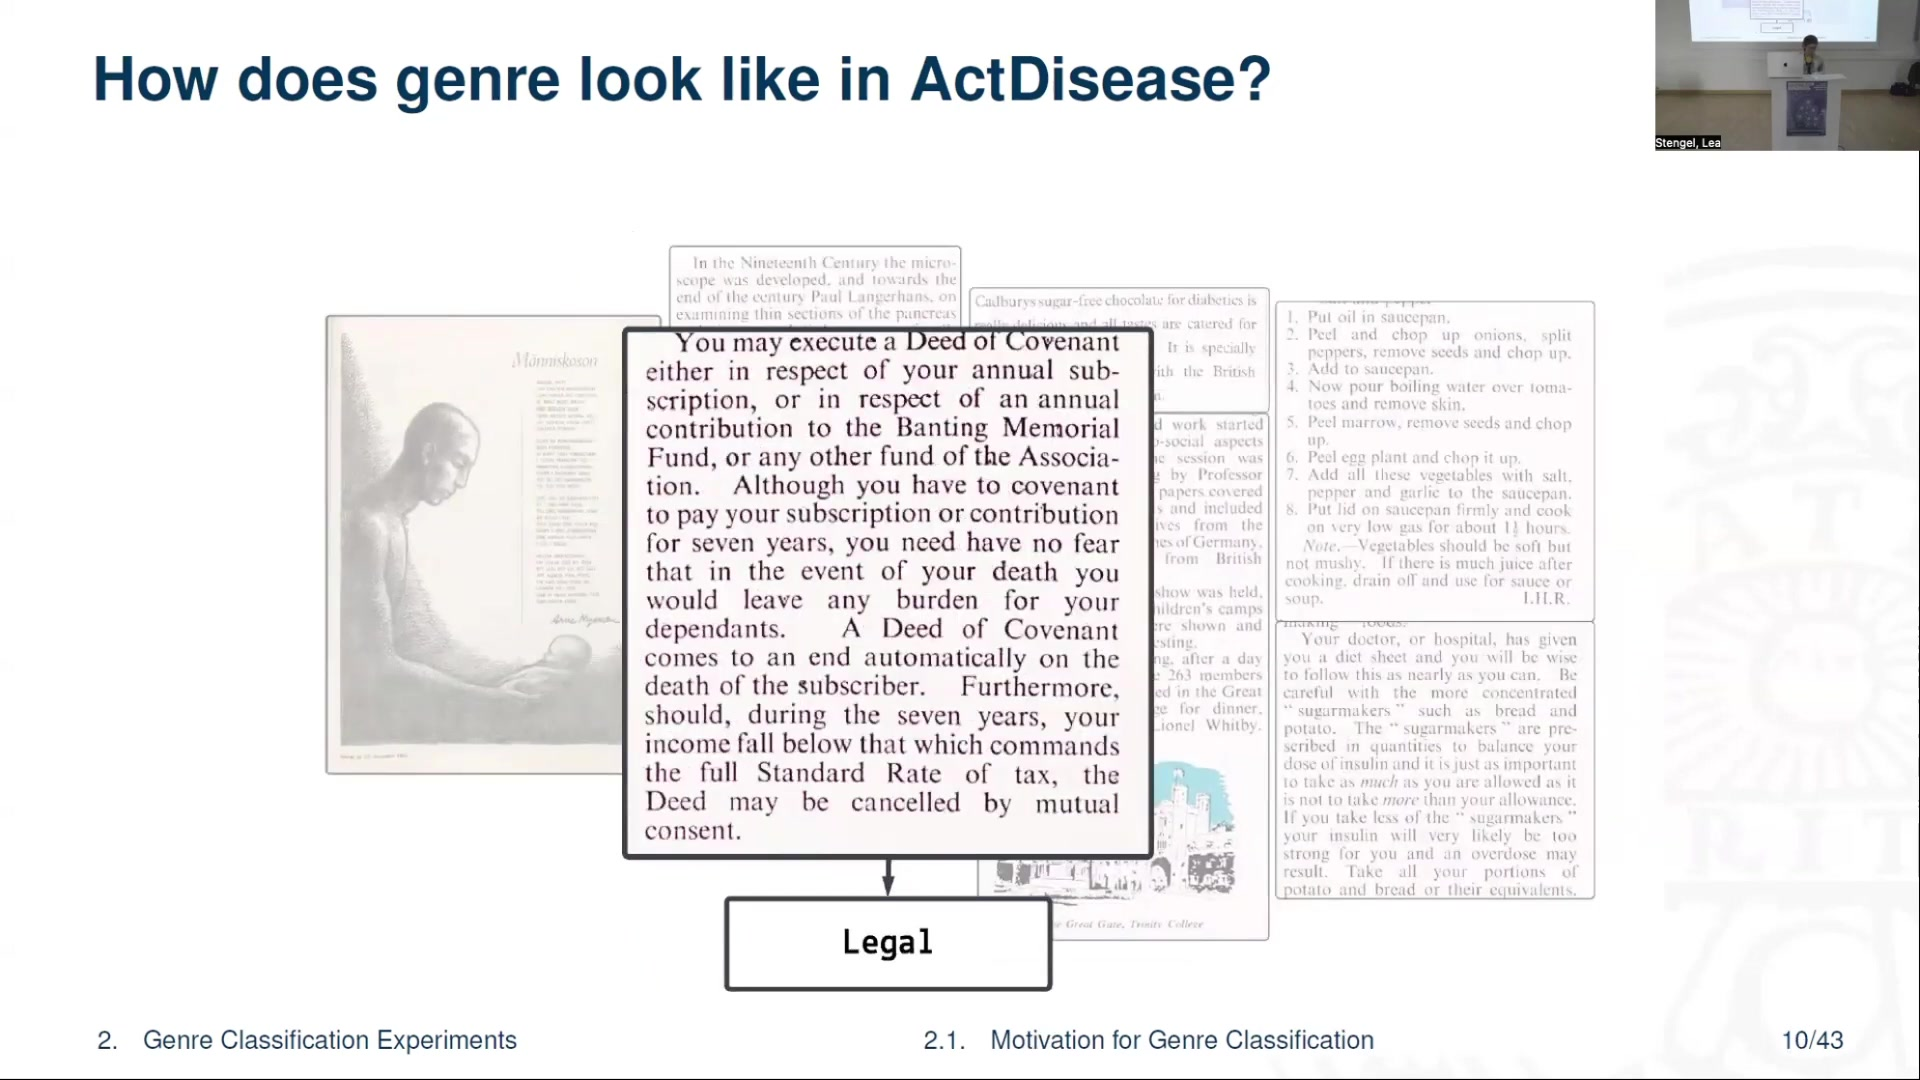
\includegraphics[keepaspectratio]{images/ai-nepi_005_slide_22.jpg}}

}

\caption{Introduction slide for Zero-Shot Learning Evaluation.}

\end{figure}%

Overall, models fine-tuned on the Functional Text Dimensions (FTD)
dataset, using the established mapping, performed better. In most FTD
configurations, researchers observed no systematic bias, and per-genre
metrics were quite good. An interesting observation emerged: on certain
datasets, some models handled specific genres much more effectively than
others on average. For instance, XLM-RoBERTa demonstrated superior
prediction of `QA' (Question \& Answer) texts compared to other models
when fine-tuned on UDM. Conversely, hmBERT, when fine-tuned on UDM,
showed a 16\% average increase in correct `Administrative' predictions
over XLM-RoBERTa and mBERT. Models based on the CORE dataset proved
adept at predicting the `Legal' genre. However, researchers noted
class-specific biases in other datasets: UDM fine-tuning tended towards
`News' (as the `News' training data had the highest number of Germanic
instances, mostly German), whilst CORE fine-tuning leaned towards
`Guide' (as only `Guide' training data in CORE was multilingual).

\begin{figure}[H]

{\centering \pandocbounded{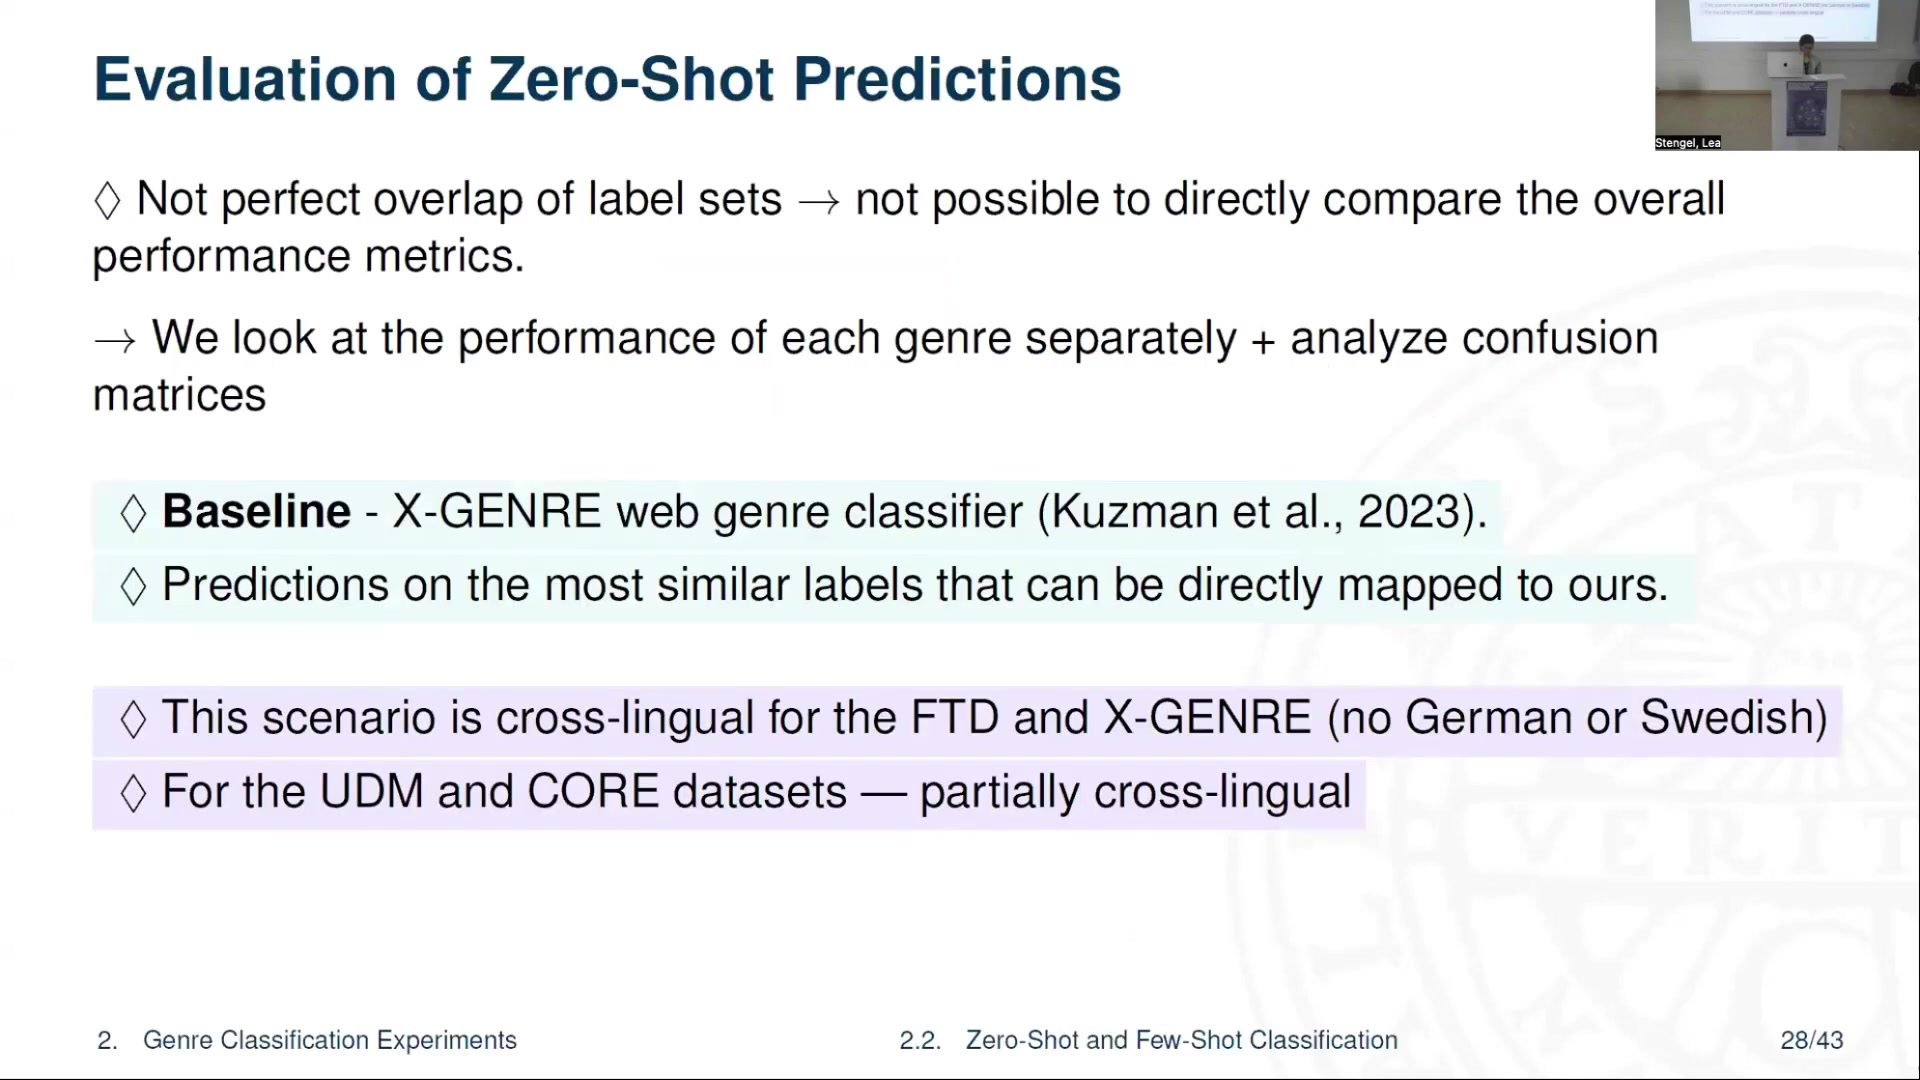
\includegraphics[keepaspectratio]{images/ai-nepi_005_slide_24.jpg}}

}

\caption{Slide summarising key results from zero-shot learning,
highlighting performance with FTD and specific model-dataset-genre
strengths.}

\end{figure}%

Confusion matrices for specific configurations illustrate this
behaviour. For example, hmBERT fine-tuned on UDM
(hmbert\_UDM\_True\_True) shows strong performance for `Administrative'.
XLM-RoBERTa fine-tuned on CORE (xlmr\_CORE\_True\_False) effectively
identifies `Legal' and `Academic' texts. XLM-RoBERTa fine-tuned on UDM
(xlmr\_UDM\_False\_False) excels with `QA'. Finally, XLM-RoBERTa
fine-tuned on FTD (xlmr\_FTD\_False\_False) accurately classifies
`Legal' texts.

\begin{figure}[H]

{\centering \pandocbounded{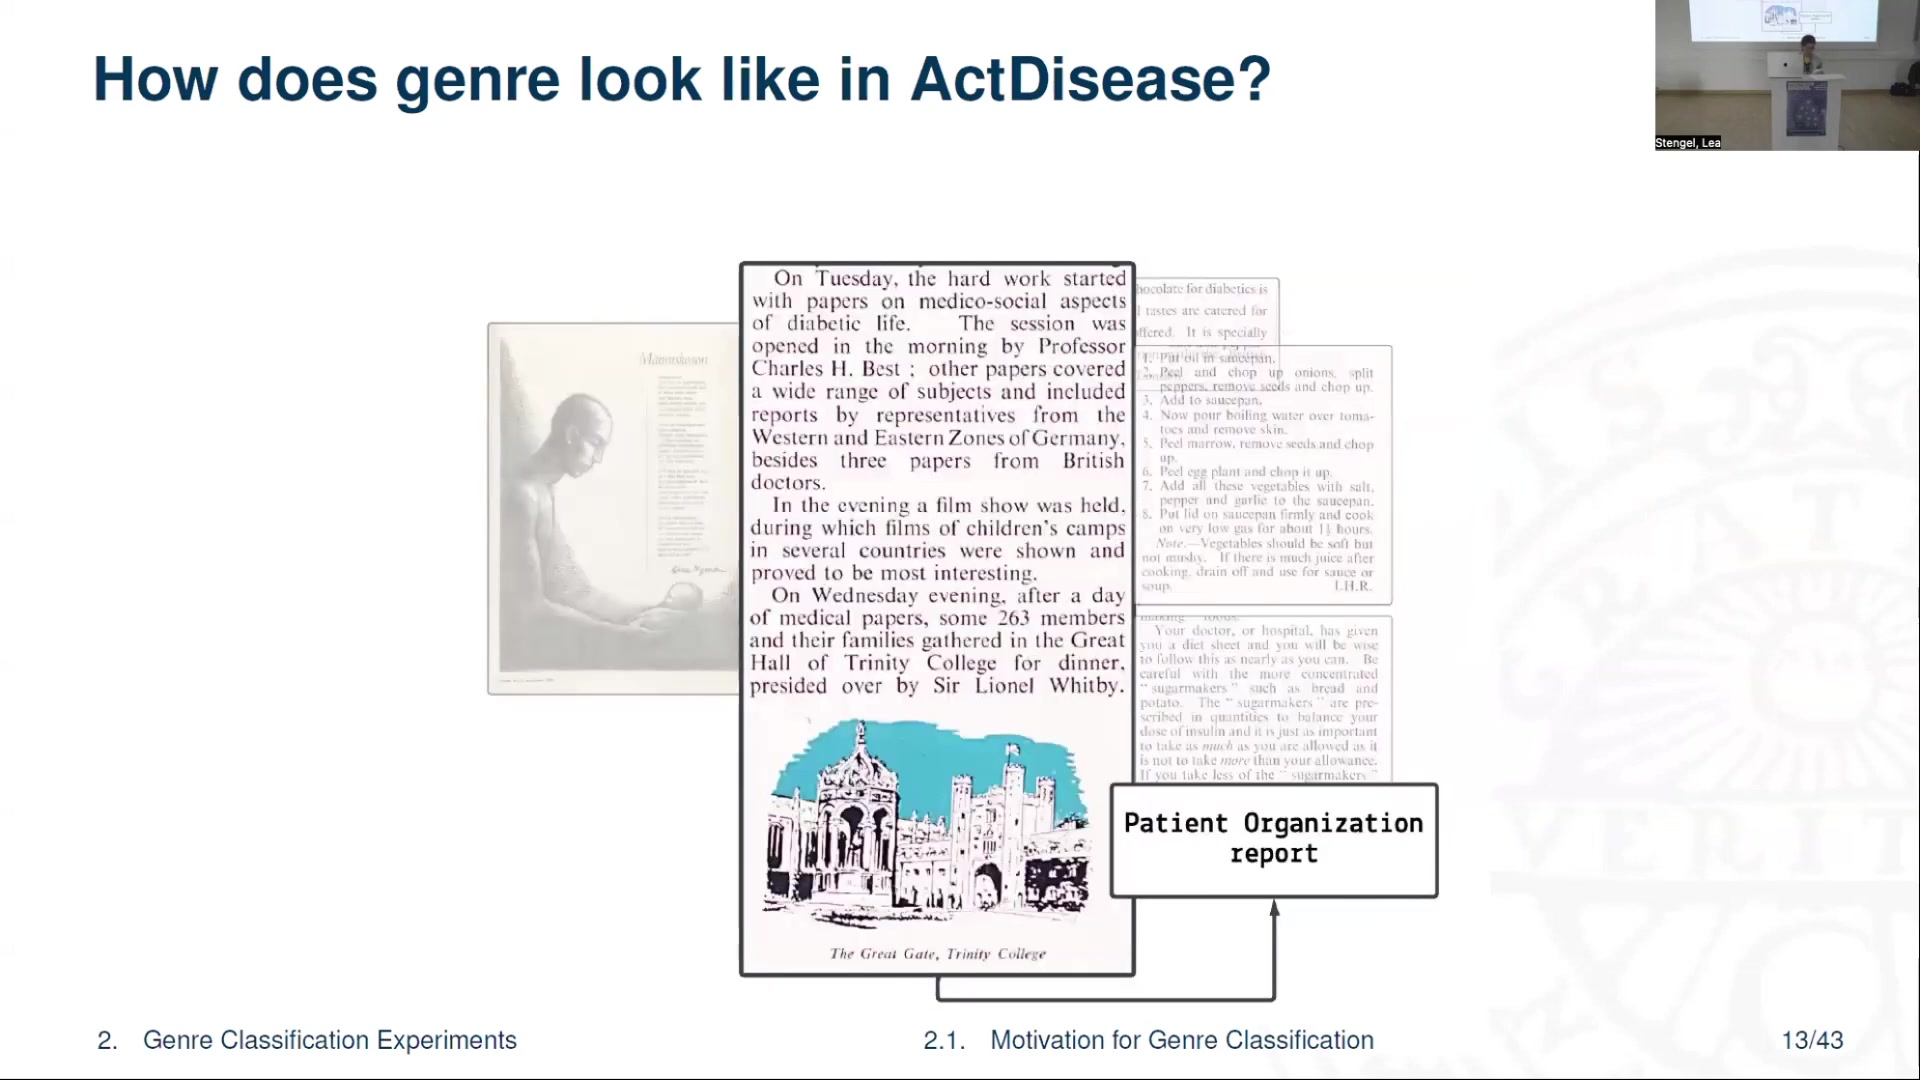
\includegraphics[keepaspectratio]{images/ai-nepi_005_slide_25.jpg}}

}

\caption{Slide displaying four confusion matrices for different model
configurations in zero-shot learning, highlighting specific genre
prediction strengths.}

\end{figure}%

The table below presents detailed average F1 scores per category,
averaged across data configurations. Highlighted values in the original
presentation (not reproduced here as bold text) indicate performance
that is not a result of systematic biases towards those categories.
Notably, models fine-tuned on FTD and CORE show strong F1 scores for the
`Legal' genre. hmBERT (UDM) performs well for `Administrative', and
XLM-RoBERTa (UDM) for `QA'.

\begin{figure}[H]

{\centering \pandocbounded{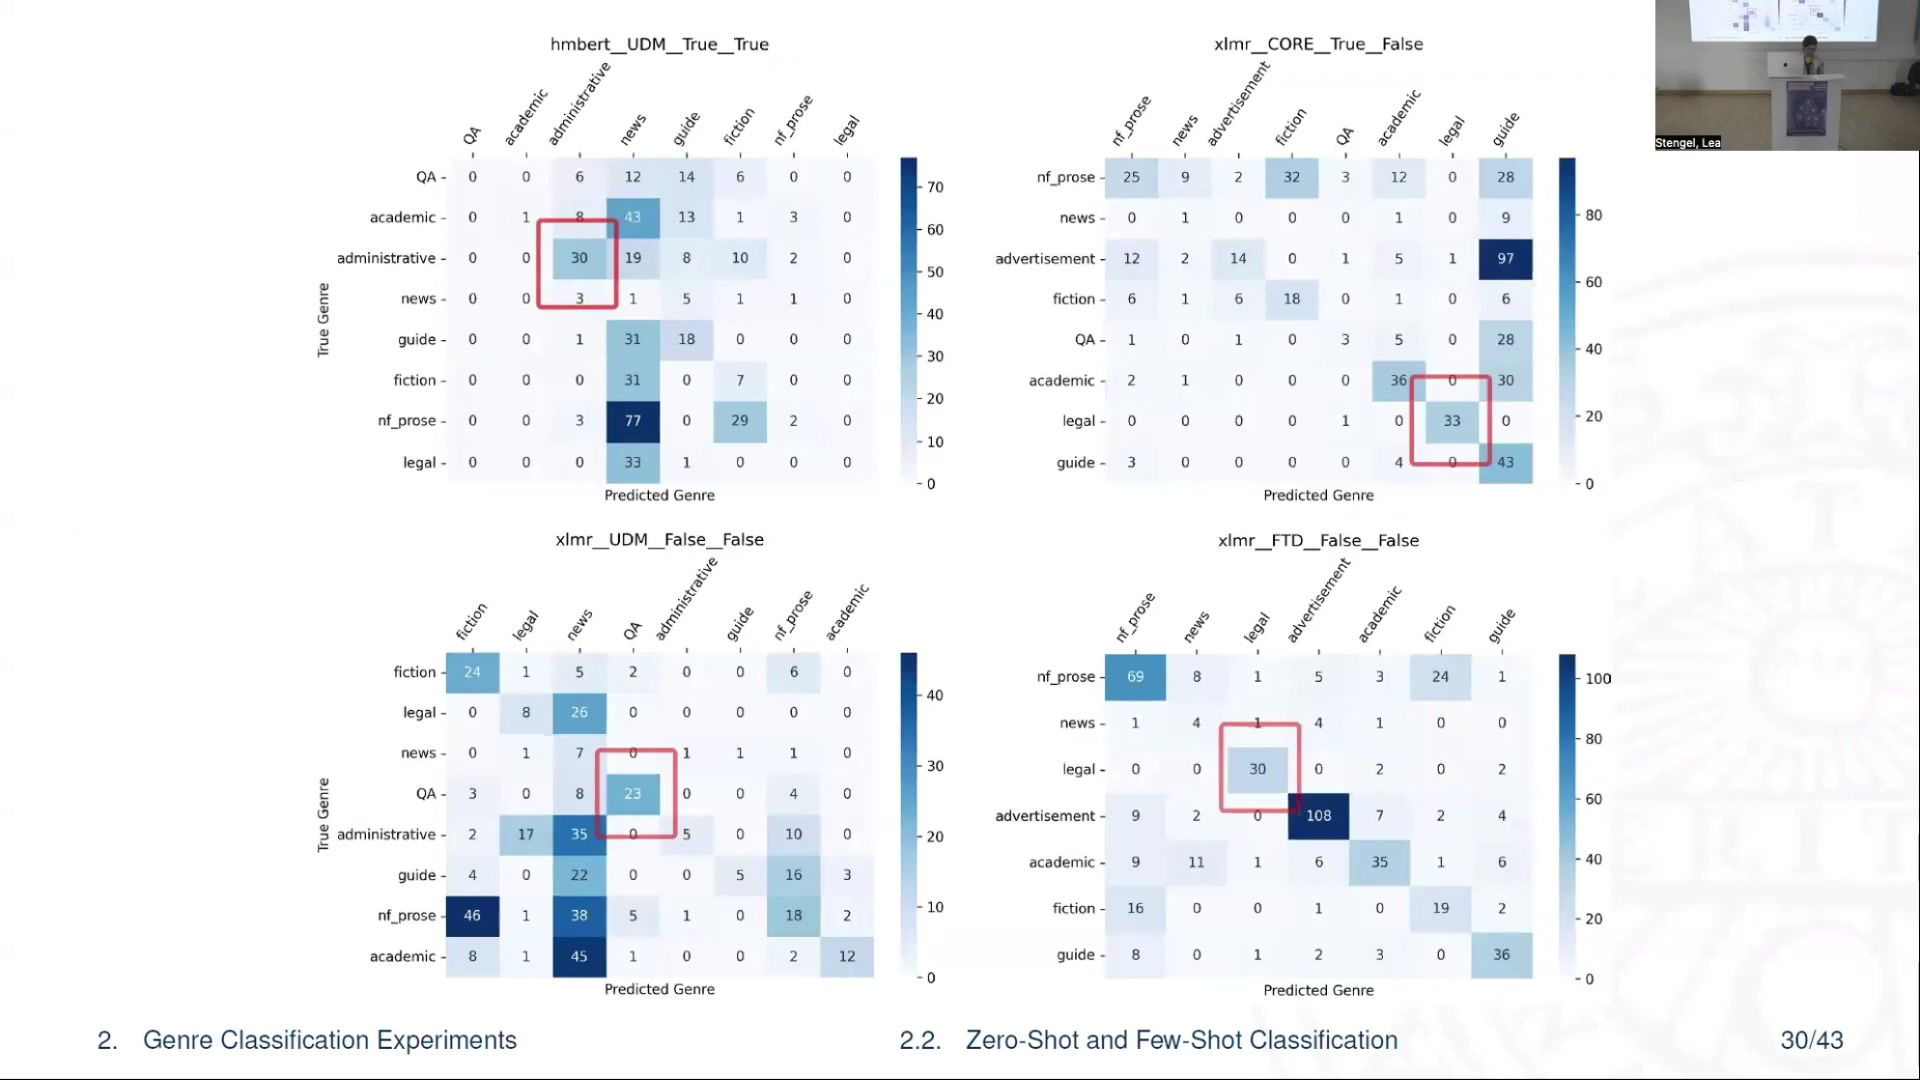
\includegraphics[keepaspectratio]{images/ai-nepi_005_slide_26.jpg}}

}

\caption{Table of zero-shot per-category F1 scores averaged across data
configurations for different models and datasets.}

\end{figure}%

Analysis of average performance across different training configurations
(balancing strategies, language family inclusion) for each external
dataset (FTD, CORE, UDM) reveals nuances. For FTD, balancing by original
labels alongside ActDisease labels ({[}B2{]}) or including only Germanic
languages ({[}G+{]}) decreased performance compared to balancing by
ActDisease labels alone ({[}B1{]}) or including all language families
({[}G-{]}). For CORE, the small number of Finnish and French instances
(in the `Guide' genre) slightly decreased performance. For UDM, the
presence of other language families and balancing generally improved
performance in terms of macro F1.

\begin{figure}[H]

{\centering \pandocbounded{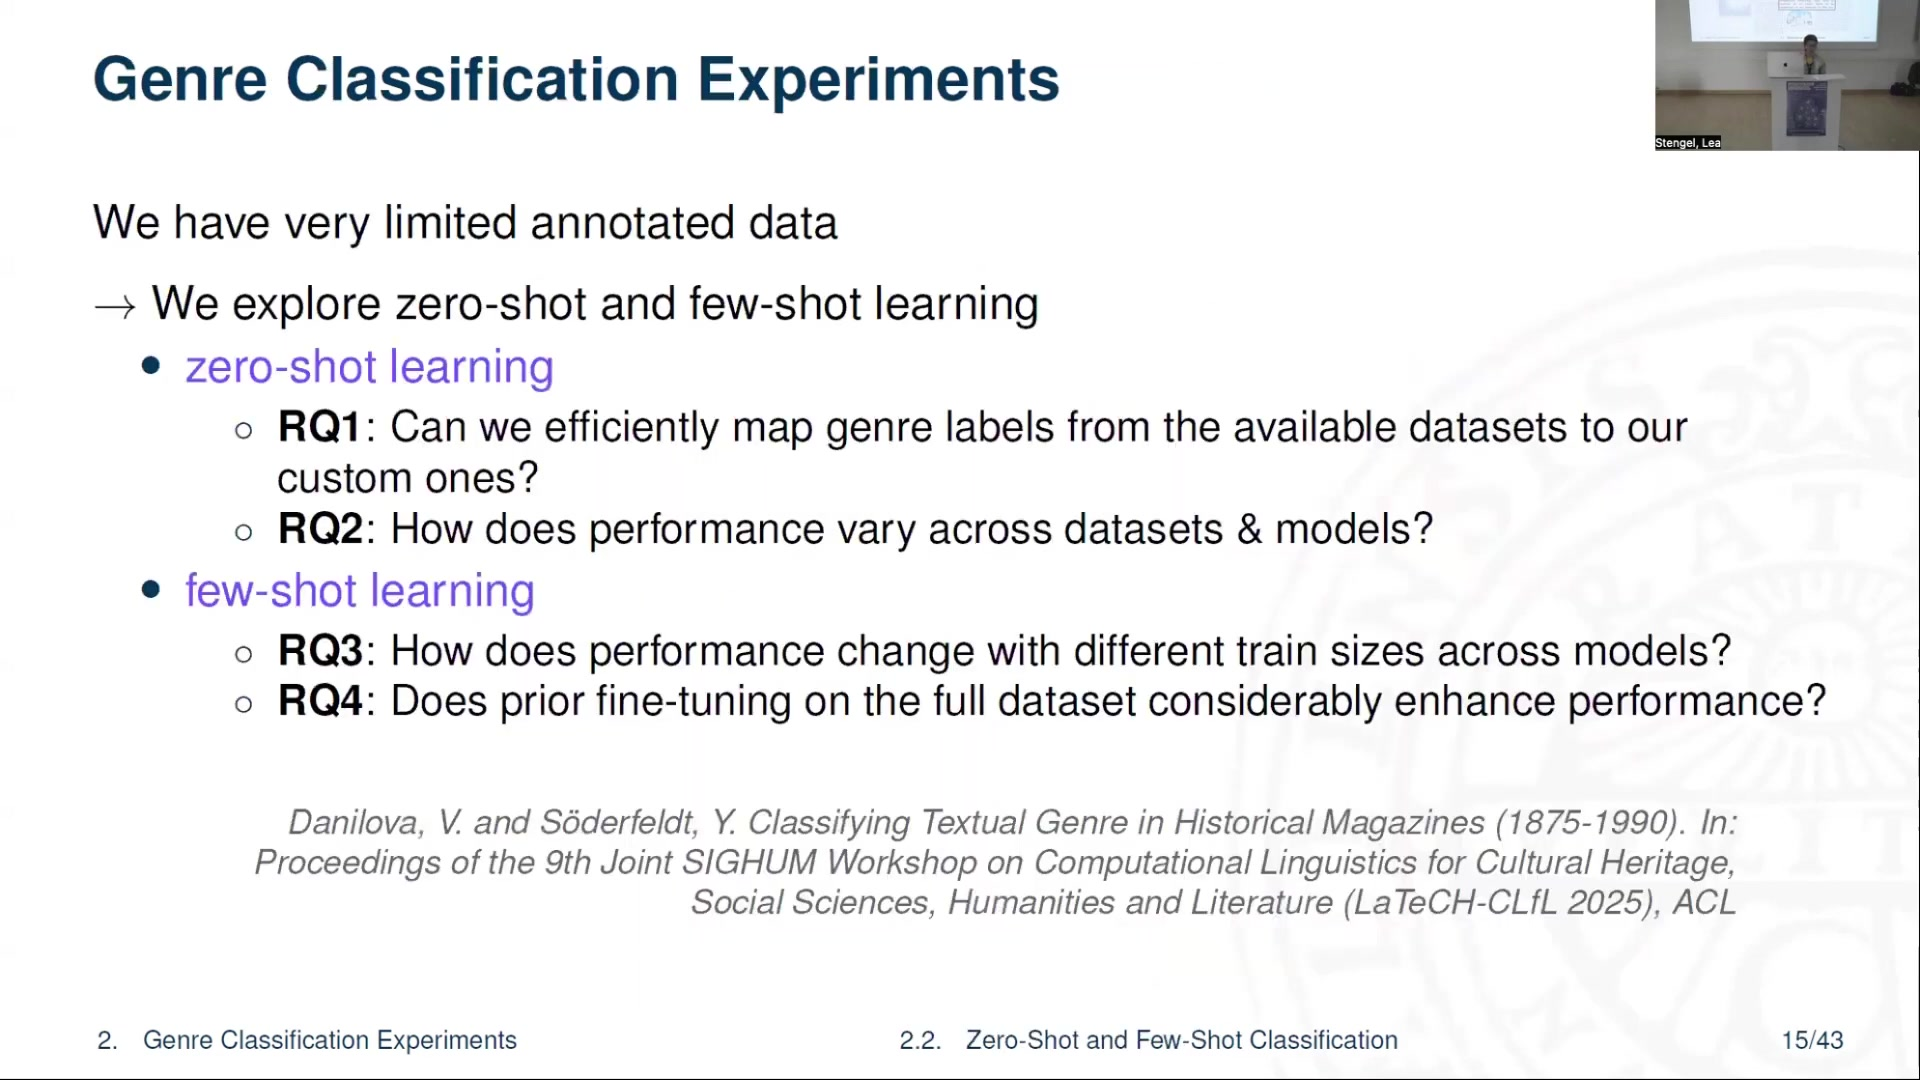
\includegraphics[keepaspectratio]{images/ai-nepi_005_slide_27.jpg}}

}

\caption{Slide showing average F1 scores for different training
configurations within FTD, CORE, and UDM datasets.}

\end{figure}%

\subsubsection{Few-Shot Learning
Evaluation}\label{few-shot-learning-evaluation}

The investigation then turned to few-shot learning scenarios.

\begin{figure}[H]

{\centering \pandocbounded{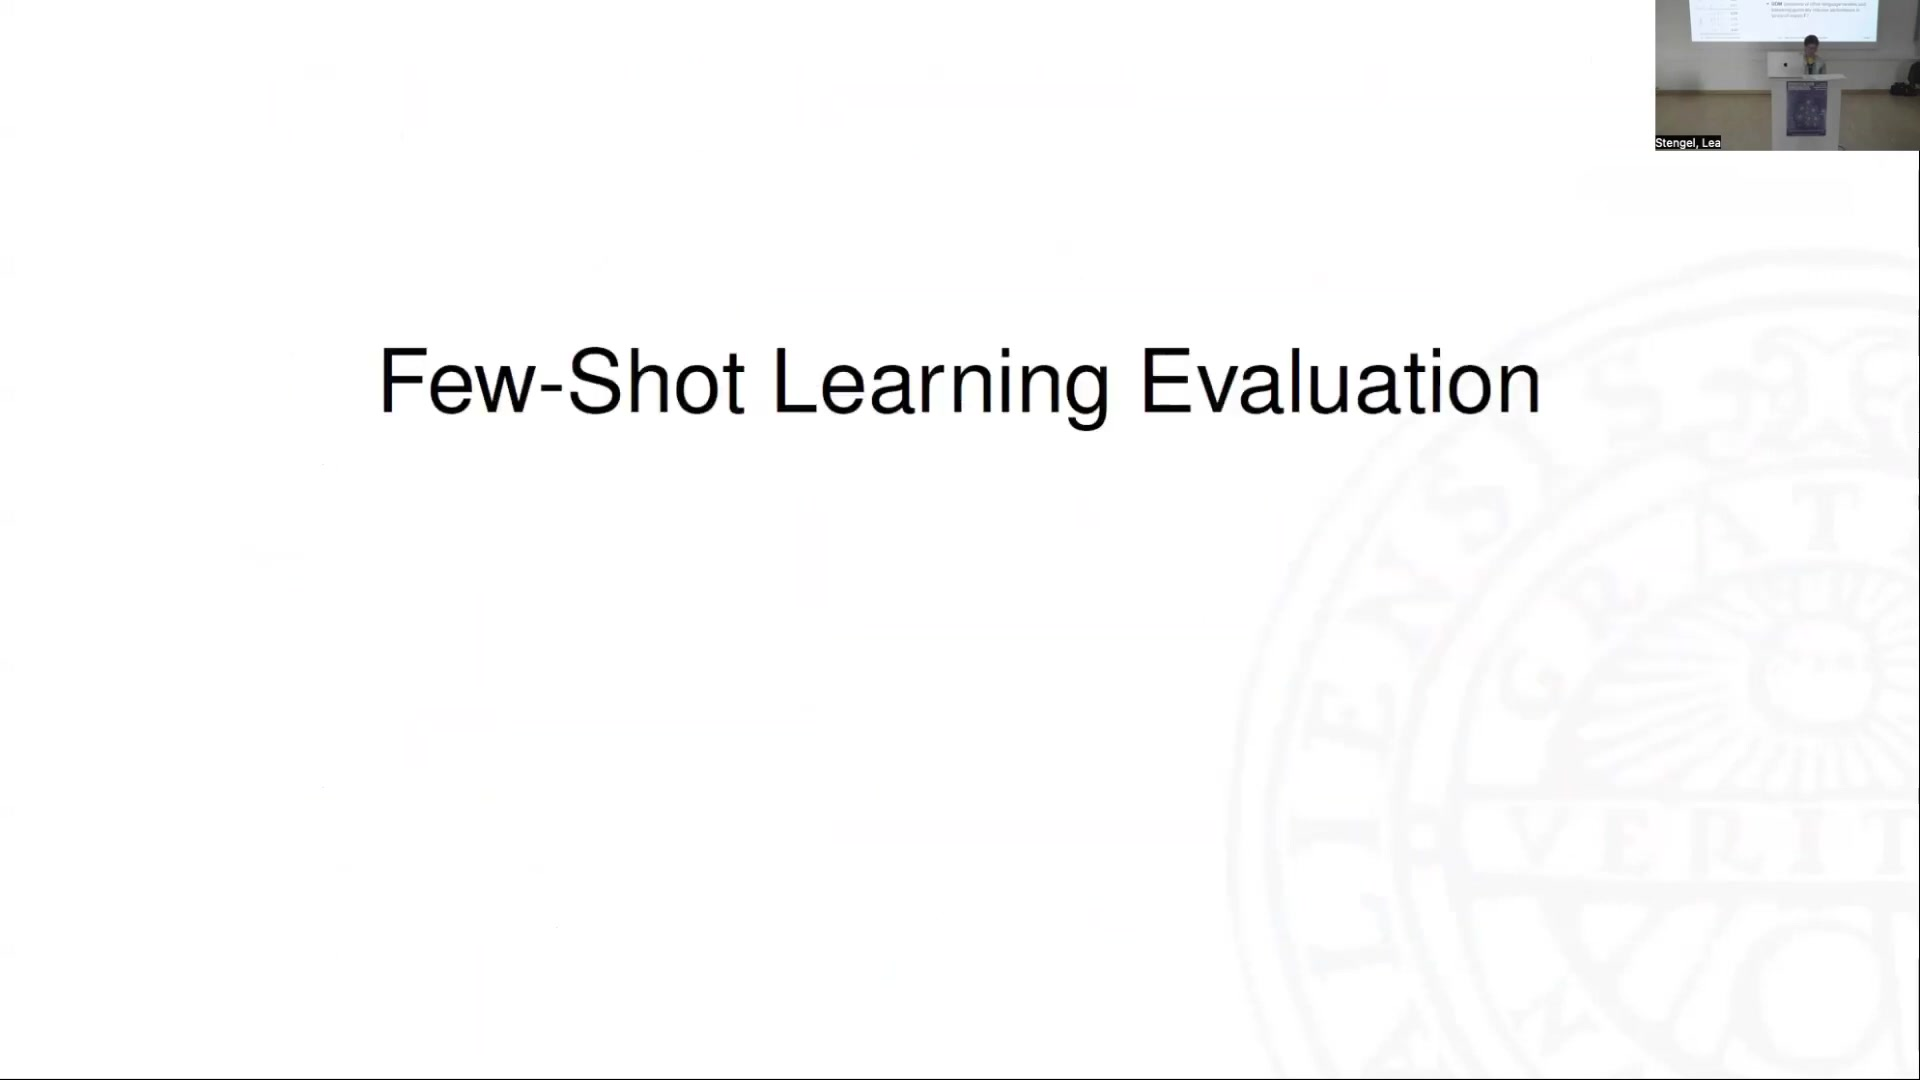
\includegraphics[keepaspectratio]{images/ai-nepi_005_slide_28.jpg}}

}

\caption{Introduction slide for Few-Shot Learning Evaluation.}

\end{figure}%

Experiments demonstrated how models performed with varying training data
sizes, both with and without prior Masked Language Model (MLM)
fine-tuning on the entire ActDisease dataset. This prior MLM fine-tuning
(+MLM) proved clearly advantageous. F1 scores generally increased with
the number of training instances, although they remained below 0.8 even
with 1182 instances. Notably, hmBERT-MLM (the historical model with
prior fine-tuning) outperformed other models, particularly at larger
dataset sizes, boosting its performance significantly and even
surpassing other models by a small margin.

\begin{figure}[H]

{\centering \pandocbounded{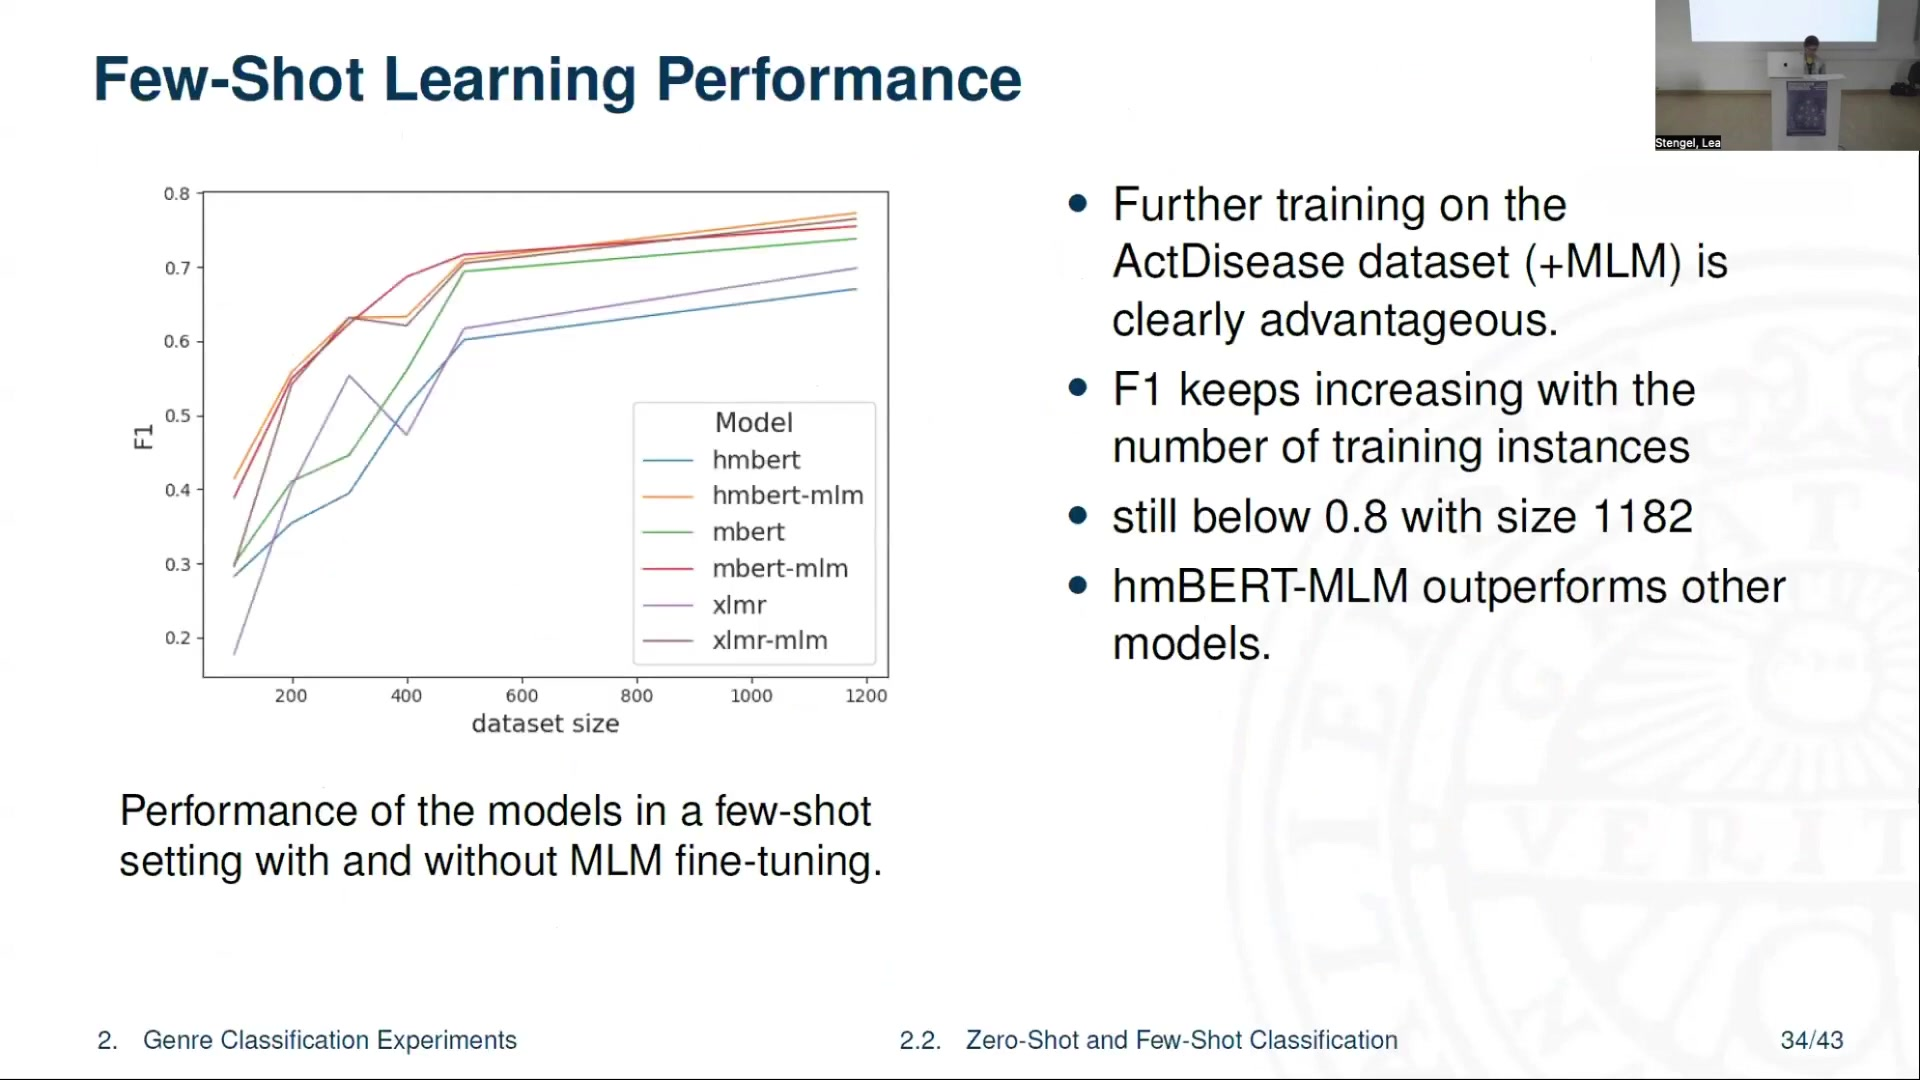
\includegraphics[keepaspectratio]{images/ai-nepi_005_slide_30.jpg}}

}

\caption{Line graph showing few-shot learning performance (F1 score
vs.~dataset size) for different models with and without MLM
fine-tuning.}

\end{figure}%

A detailed examination of scores revealed that hmBERT-MLM's superior
performance is largely attributable to its sustained ability to
differentiate between `Fiction' and `Nonfiction Prose' as dataset size
increases. In contrast, other models, especially XLM-RoBERTa-MLM,
exhibited a drastic drop in performance for `Fiction' when using the
full-sized training dataset (1182 instances), often over-predicting
`Nonfiction Prose' for `Fiction' instances. Both these genres in the
ActDisease data frequently contain narratives about patient experiences,
particularly concerning diabetes. It is plausible that with a larger
data size, the linguistic features of these two genres become more
similar, especially as they are confined to the specific domain of
patient organisation magazines focused on diabetes and often share
themes and narrative structures. This suggests that more data, or
perhaps more nuanced features, might be necessary to improve
discrimination between these closely related genres.

\pandocbounded{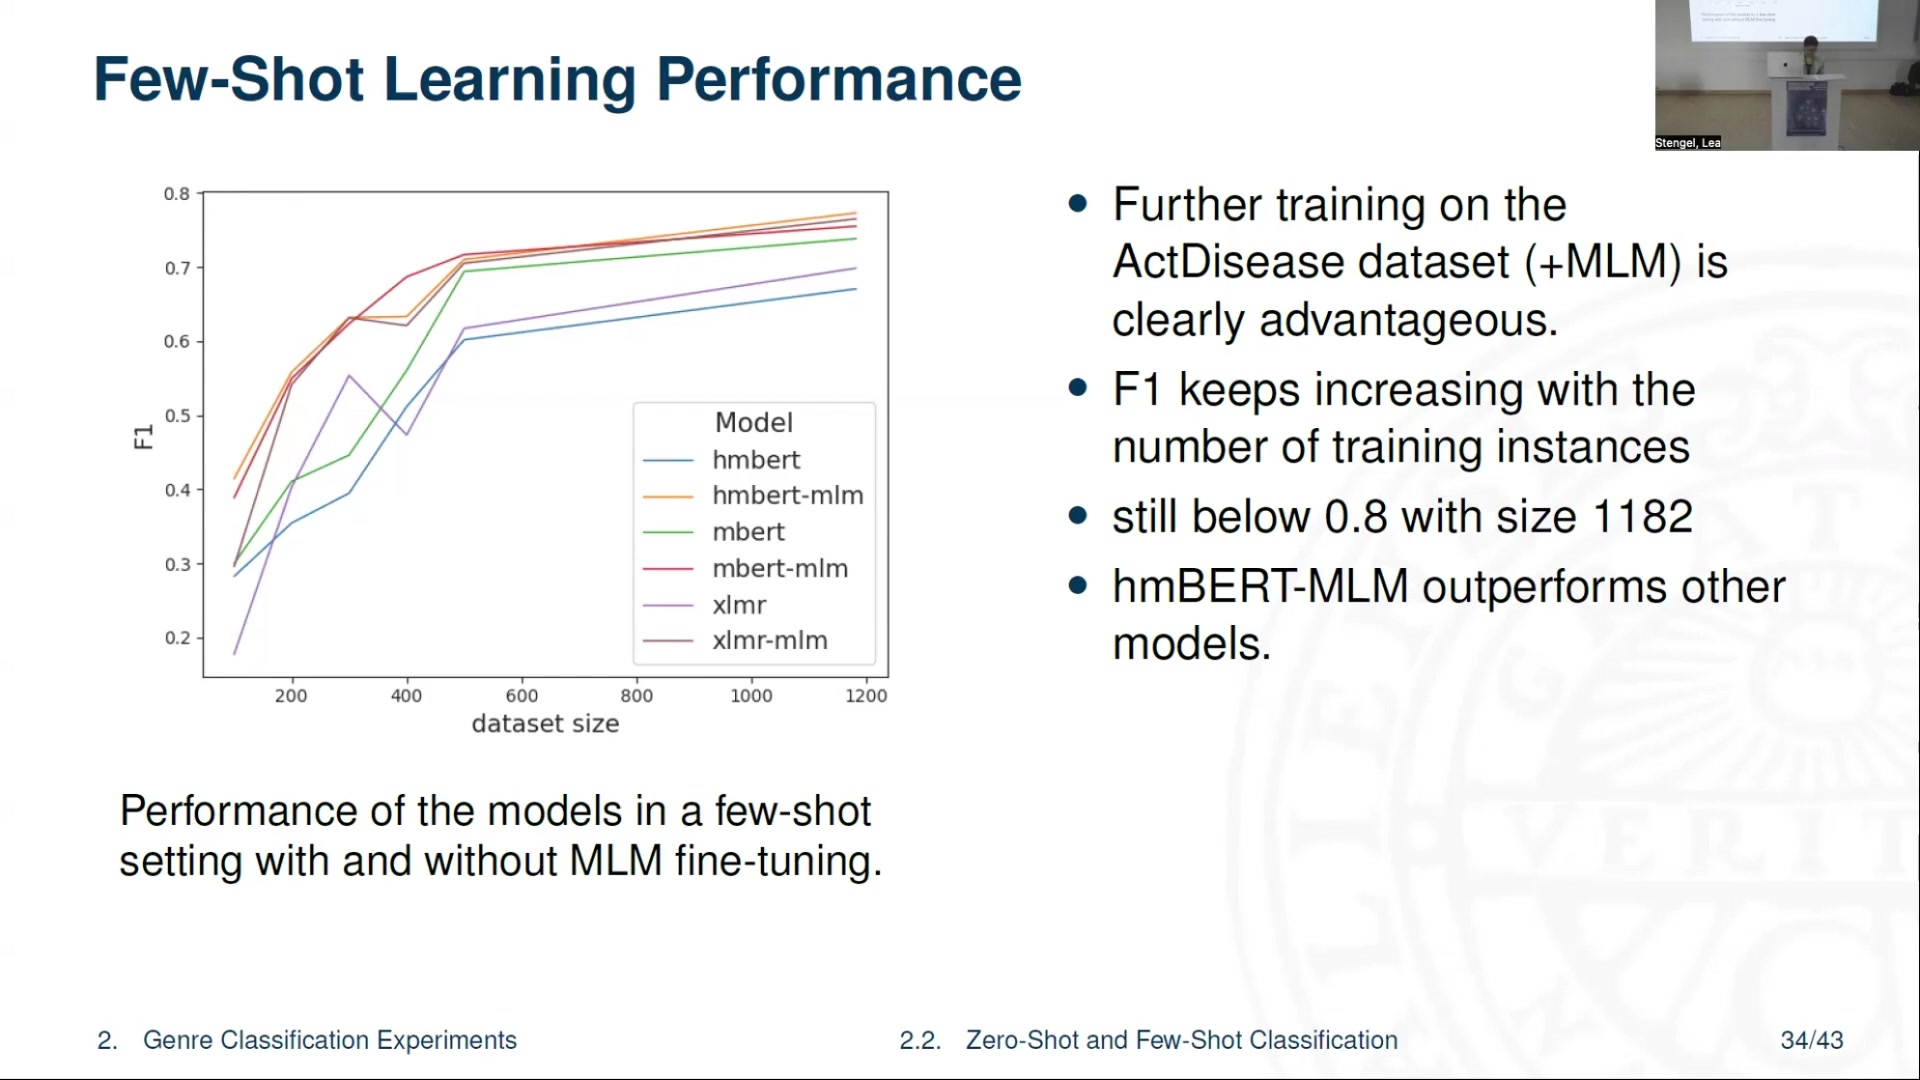
\includegraphics[keepaspectratio]{images/ai-nepi_005_slide_31.jpg}}
\pandocbounded{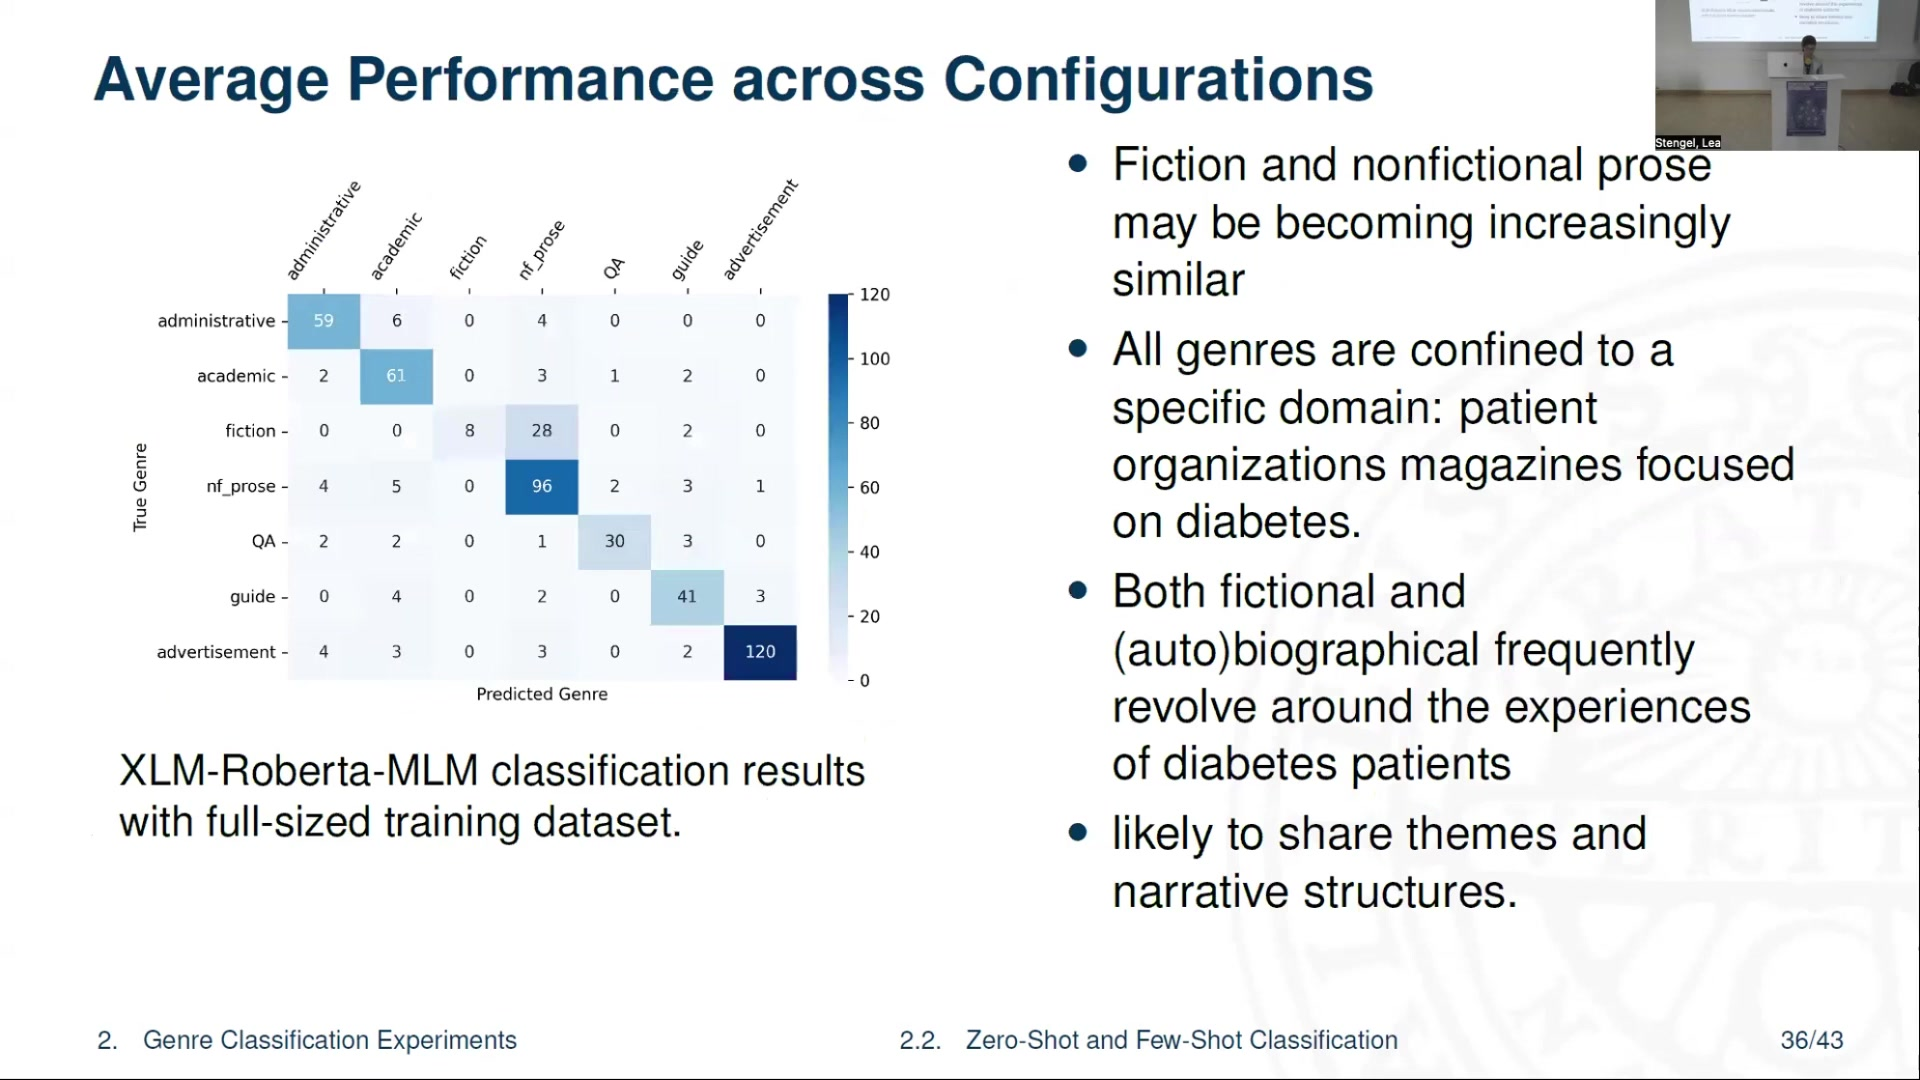
\includegraphics[keepaspectratio]{images/ai-nepi_005_slide_32.jpg}}

\subsection{Few-Shot Prompting Llama-3.1 8b
Instruct}\label{few-shot-prompting-llama-3.1-8b-instruct}

Recognising the limitations of available data for extensive instruction
tuning, researchers also explored few-shot prompting with Llama-3.1 8b
Instruct, a prominent multilingual generative model with open weights.
The prompt structure incorporated genre definitions and two to three
carefully selected examples for each genre. The instruction guided the
model to label input text with one of the defined genres based on its
perceived purpose and content.

\begin{figure}[H]

{\centering \pandocbounded{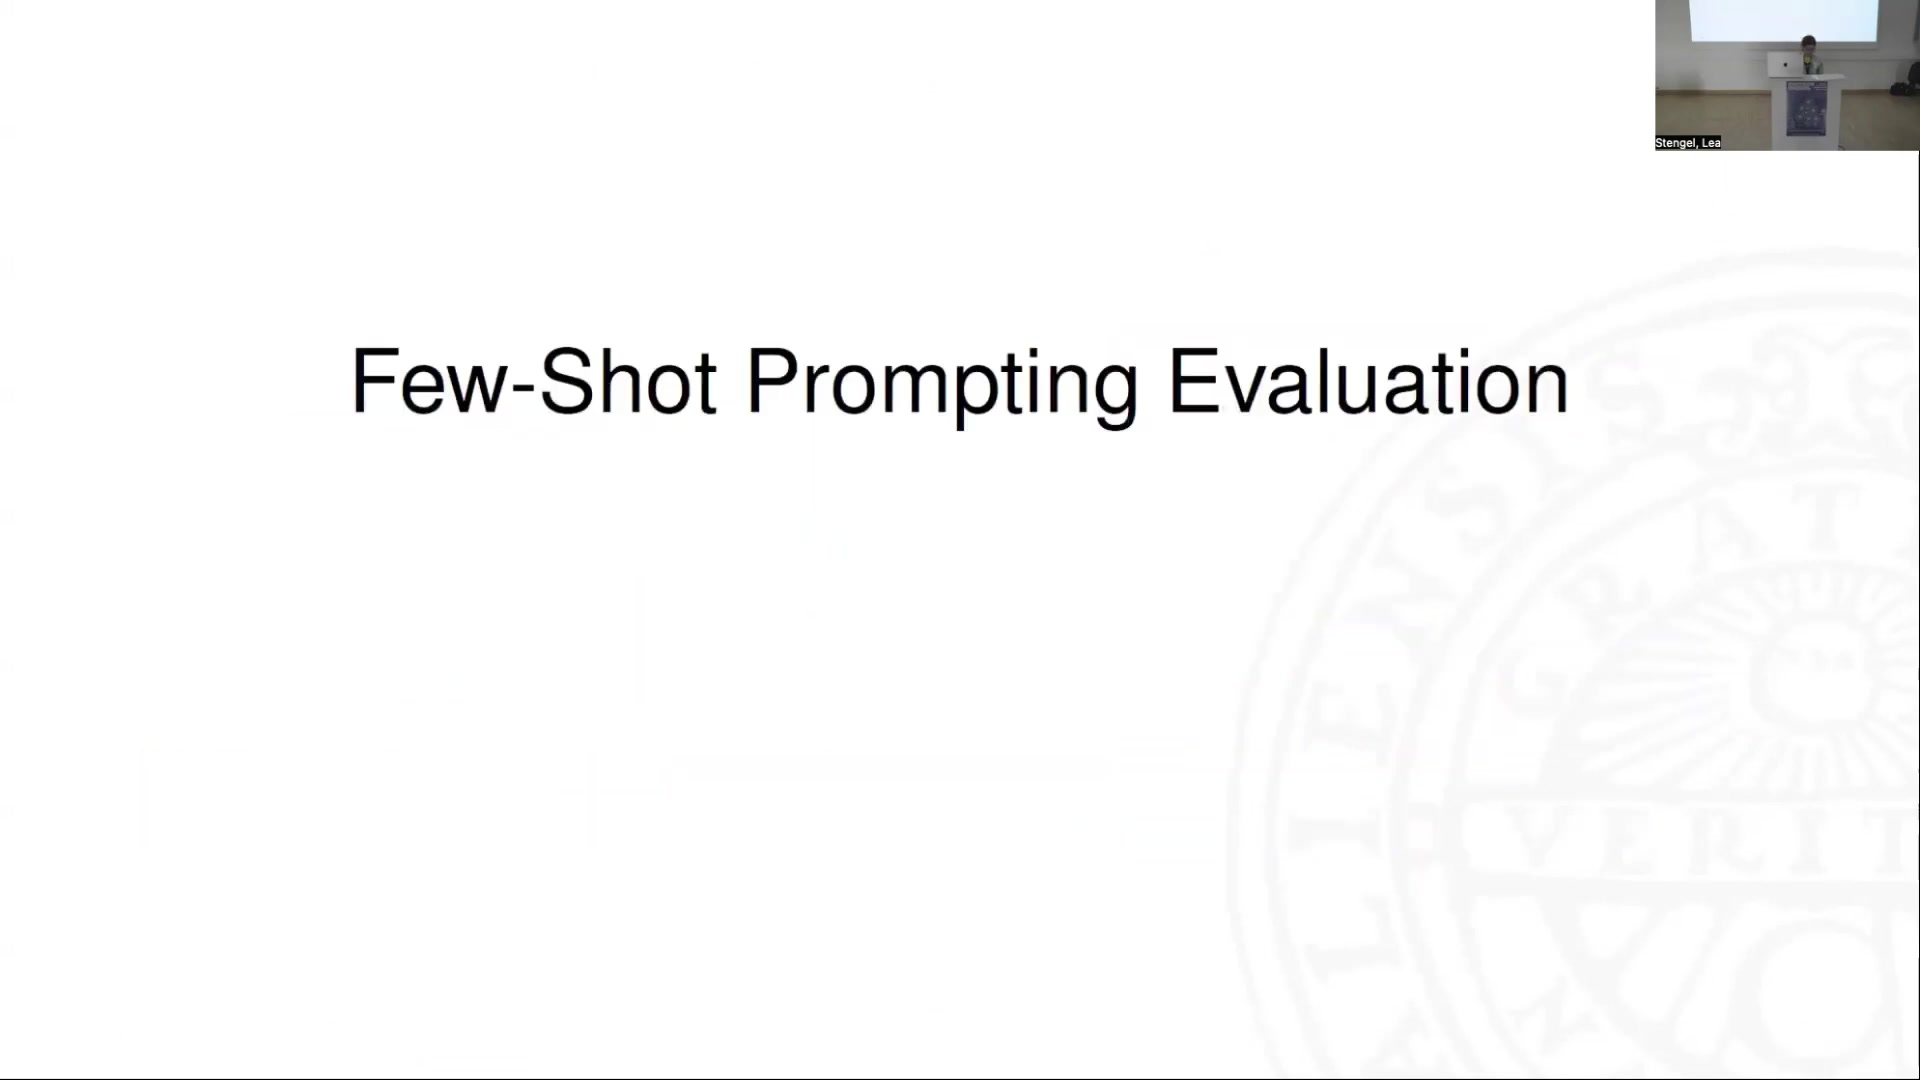
\includegraphics[keepaspectratio]{images/ai-nepi_005_slide_33.jpg}}

}

\caption{Slide illustrating the prompt structure used for few-shot
prompting of Llama-3.1 8b Instruct, including genre definitions and
example placeholders.}

\end{figure}%

The results from few-shot prompting Llama-3.1 8b Instruct on the
zero-shot test set (the entire held-out set) indicate that the model
handles certain labels reasonably well. For instance, `Legal' texts
achieved an F1-score of 0.84, and `Academic' and `Advertisement' texts
scored 0.72 and 0.73, respectively. However, the provision of only two
or three examples proved insufficient for the model to adequately
represent and distinguish more nuanced genres such as `Nonfiction Prose'
(F1-score 0.49), `Administrative' (F1-score 0.60), and `News' (F1-score
0.08). The overall macro average F1-score was 0.59. The confusion matrix
reveals particular difficulties in distinguishing `Nonfiction Prose'
from `Fiction' and `Administrative' texts, and `Advertisement' from
`Administrative' texts.

\begin{figure}[H]

{\centering \pandocbounded{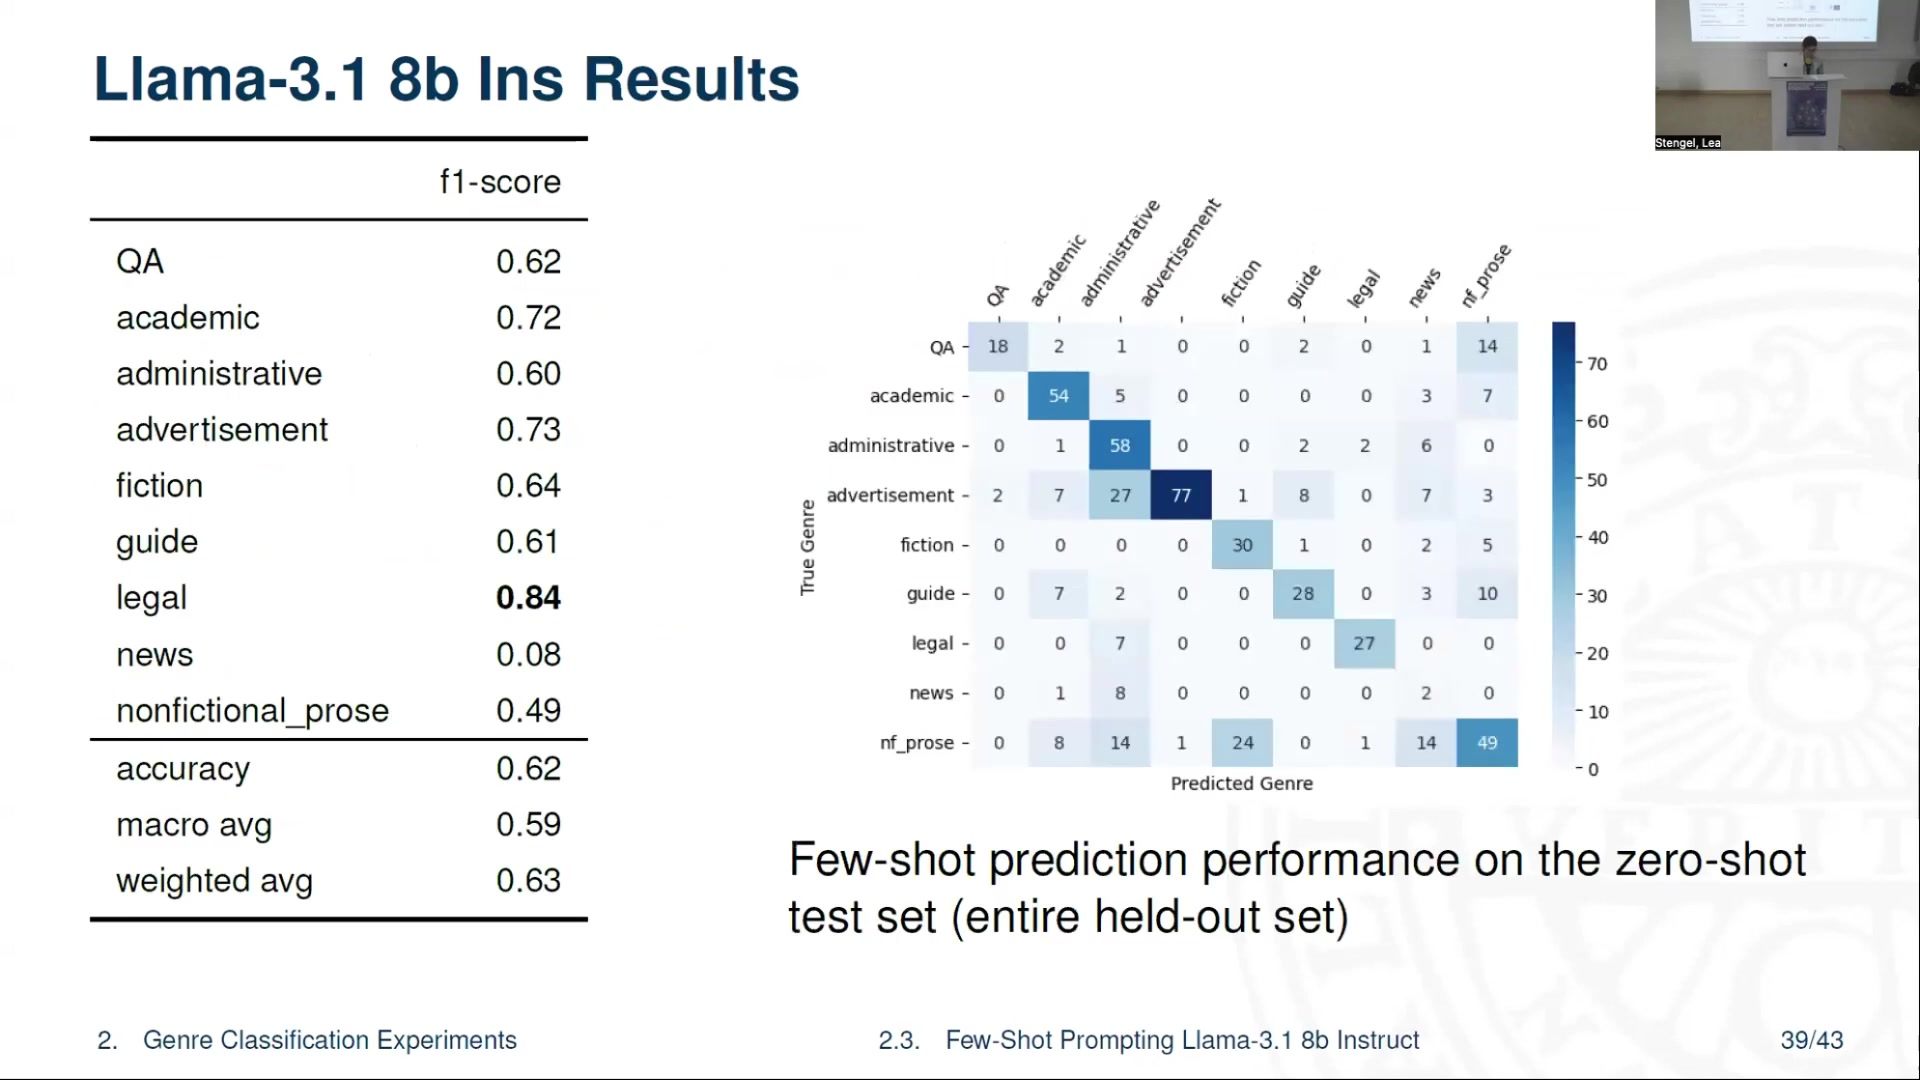
\includegraphics[keepaspectratio]{images/ai-nepi_005_slide_34.jpg}}

}

\caption{Slide presenting results (F1 scores and confusion matrix) for
few-shot prompting of Llama-3.1 8b Instruct.}

\end{figure}%

\section{Conclusion}\label{conclusion}

Historical periodicals, particularly popular magazines, represent a
promising yet challenging source for research into the history of
science and medicine. Their genre-rich nature reflects diverse
communicative strategies employed over time. Accurately accounting for
these genres is crucial for the detailed interpretation of text mining
results.

This exploration demonstrates that genre classification can
significantly enhance the accessibility of such complex historical
sources for computational analysis. When faced with no training data,
researchers can successfully leverage available modern datasets,
provided the genre categories are sufficiently general-purpose.
Alternatively, few-shot prompting of capable open generative models,
like Llama-3.1 8b Instruct, can achieve decent quality for some genres,
although performance may be limited for categories requiring more
nuanced understanding with minimal examples.

However, if some annotated data is available, even in limited
quantities, few-shot learning with multilingual encoders---such as
XLM-RoBERTa or, notably, historical multilingual BERT
(hmBERT)---especially when combined with prior Masked Language Model
(MLM) fine-tuning on the target domain data, emerges as a superior
strategy. For the ActDisease project, this approach yielded the most
promising results, with hmBERT-MLM showing considerable gains in
performance.

\begin{figure}[H]

{\centering \pandocbounded{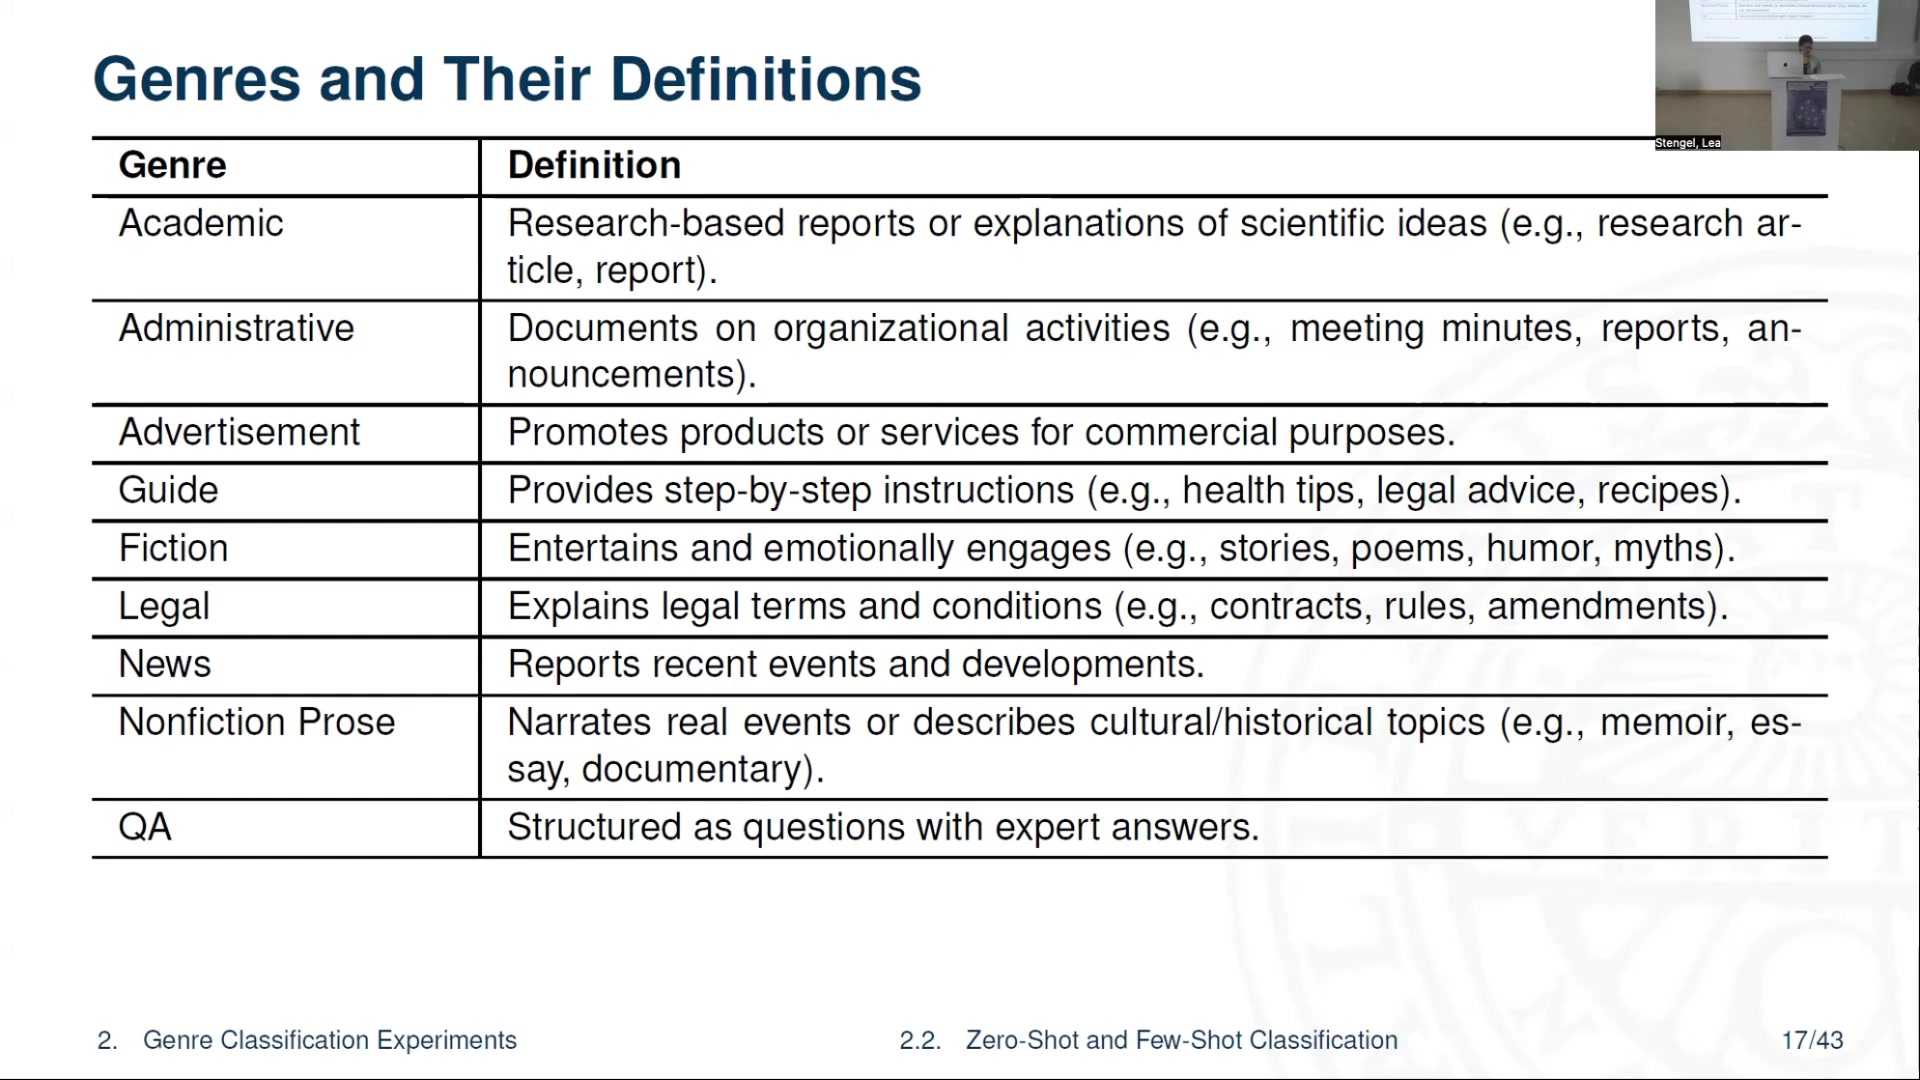
\includegraphics[keepaspectratio]{images/ai-nepi_005_slide_35.jpg}}

}

\caption{Slide summarising the main conclusions regarding genre richness
in popular magazines and effective strategies for genre classification.}

\end{figure}%

Ongoing and future efforts aim to further refine these methodologies and
apply them to specific historical hypotheses. This includes developing a
new annotation scheme with more fine-grained genres, an annotation
project financed by Swe-CLARIN, exploring synthetic data generation
techniques, and implementing active learning strategies to improve
classifier quality efficiently. These endeavours seek to enhance the
utility of these methods for both the ActDisease project and the broader
digital humanities community.

\begin{figure}[H]

{\centering \pandocbounded{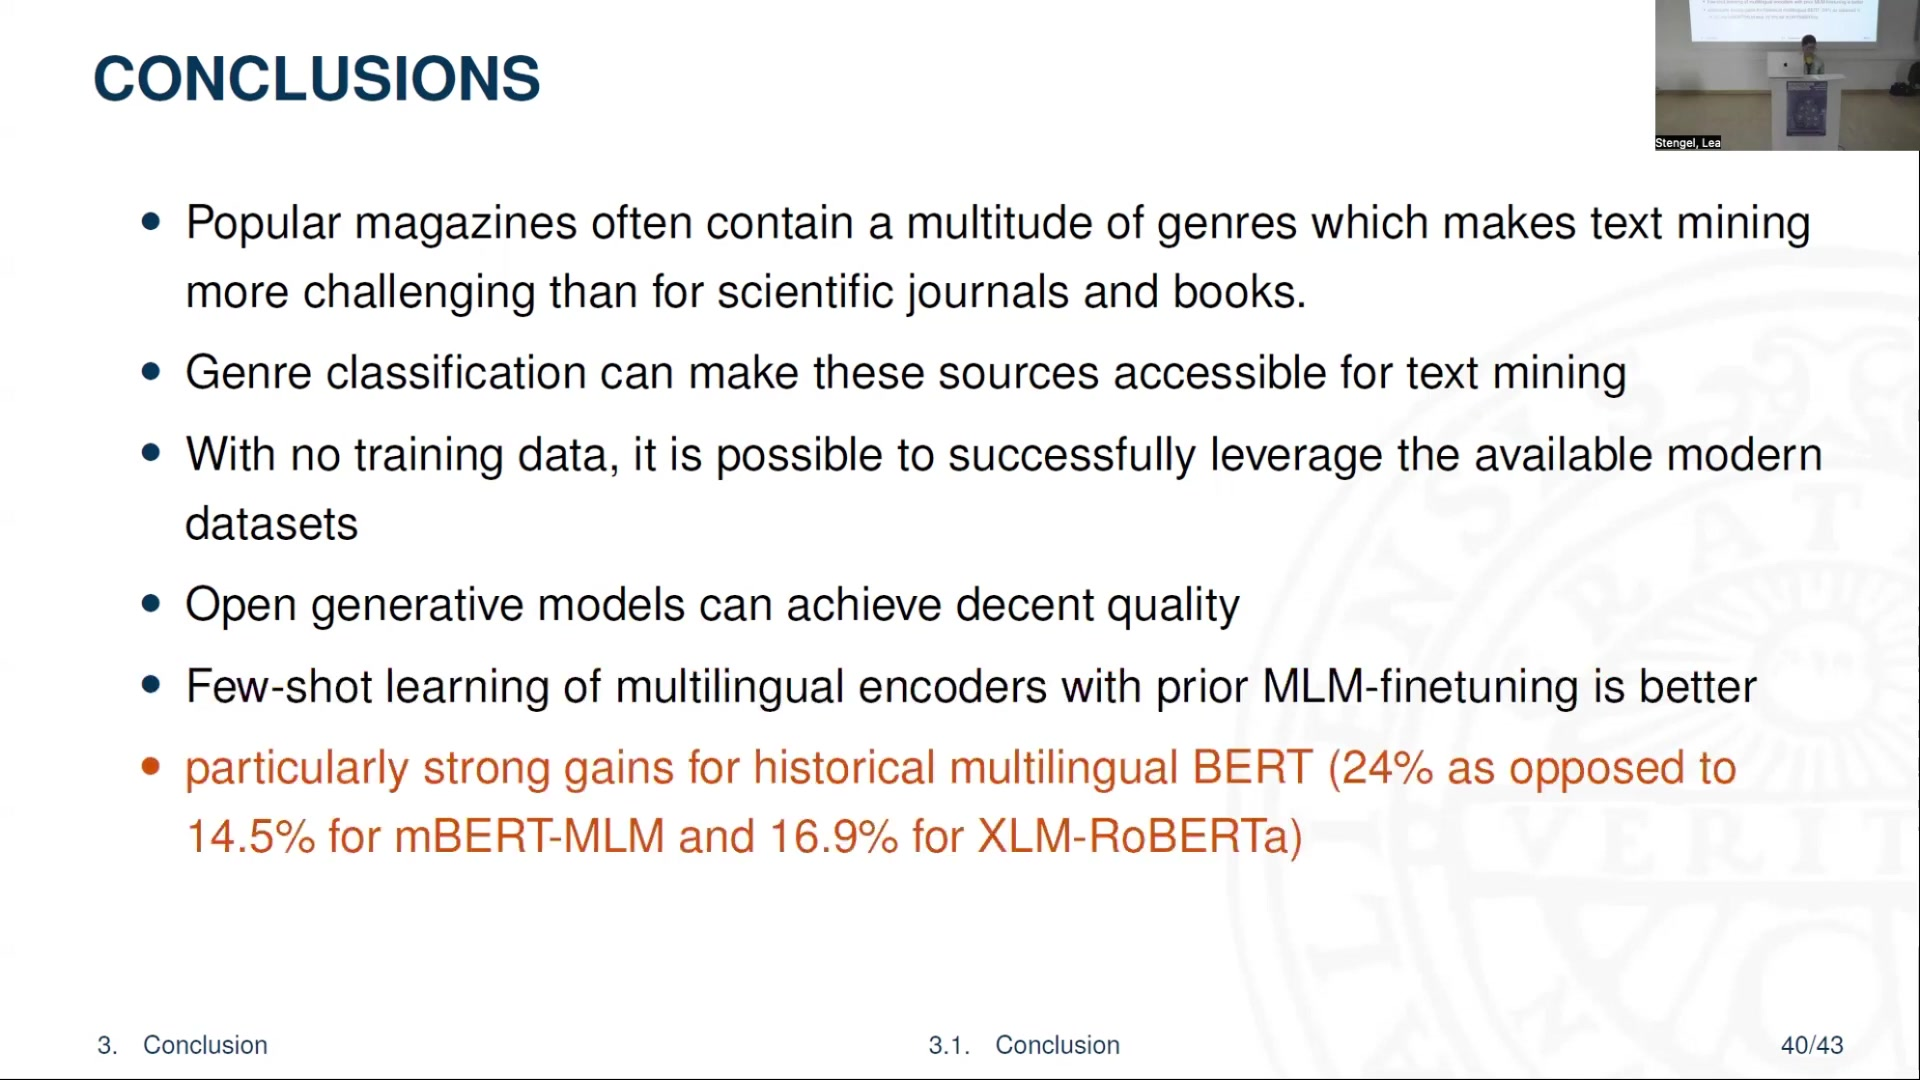
\includegraphics[keepaspectratio]{images/ai-nepi_005_slide_36.jpg}}

}

\caption{Slide outlining future and present work, including working with
historical hypotheses, new annotation schemes, and advanced machine
learning techniques.}

\end{figure}%

\subsection*{Acknowledgements}\label{acknowledgements}
\addcontentsline{toc}{subsection}{Acknowledgements}

The project team extends its gratitude to the annotators: Ylva
Söderfeldt, Julia Reed, Andrew Burchell, Maria Skeppstedt, and Gijs
Aangenendt. We also thank Dr Maria Skeppstedt and the anonymous
reviewers for their valuable feedback. This research received funding
from the European Research Council (ERC-2021-STG, 101040999). The Centre
for Digital Humanities and Social Sciences at Uppsala University
provided essential support in the form of GPUs and data storage.

\begin{figure}[H]

{\centering \pandocbounded{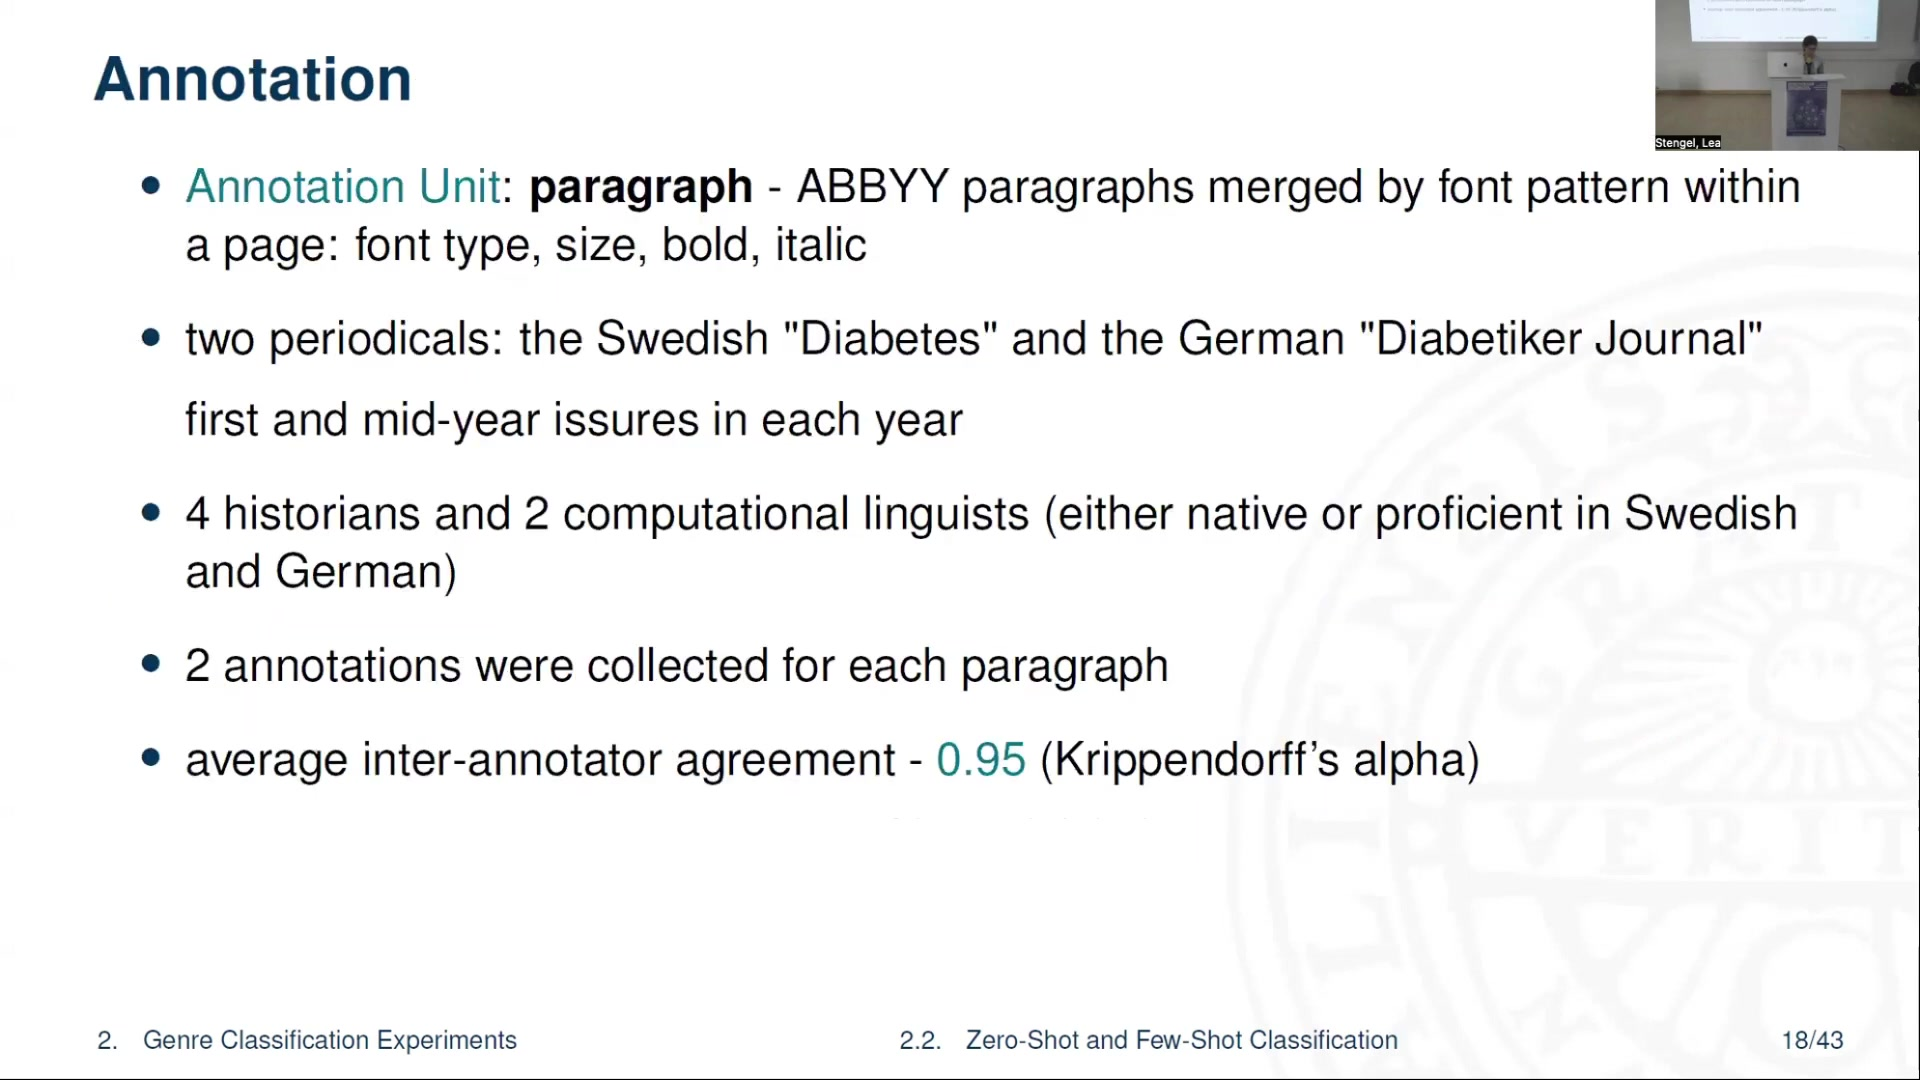
\includegraphics[keepaspectratio]{images/ai-nepi_005_slide_37.jpg}}

}

\caption{Slide listing acknowledgements to the project team, reviewers,
European Research Council, and Centre for Digital Humanities and Social
Sciences.}

\end{figure}%

For further information, please visit the project website.

\begin{figure}[H]

{\centering \pandocbounded{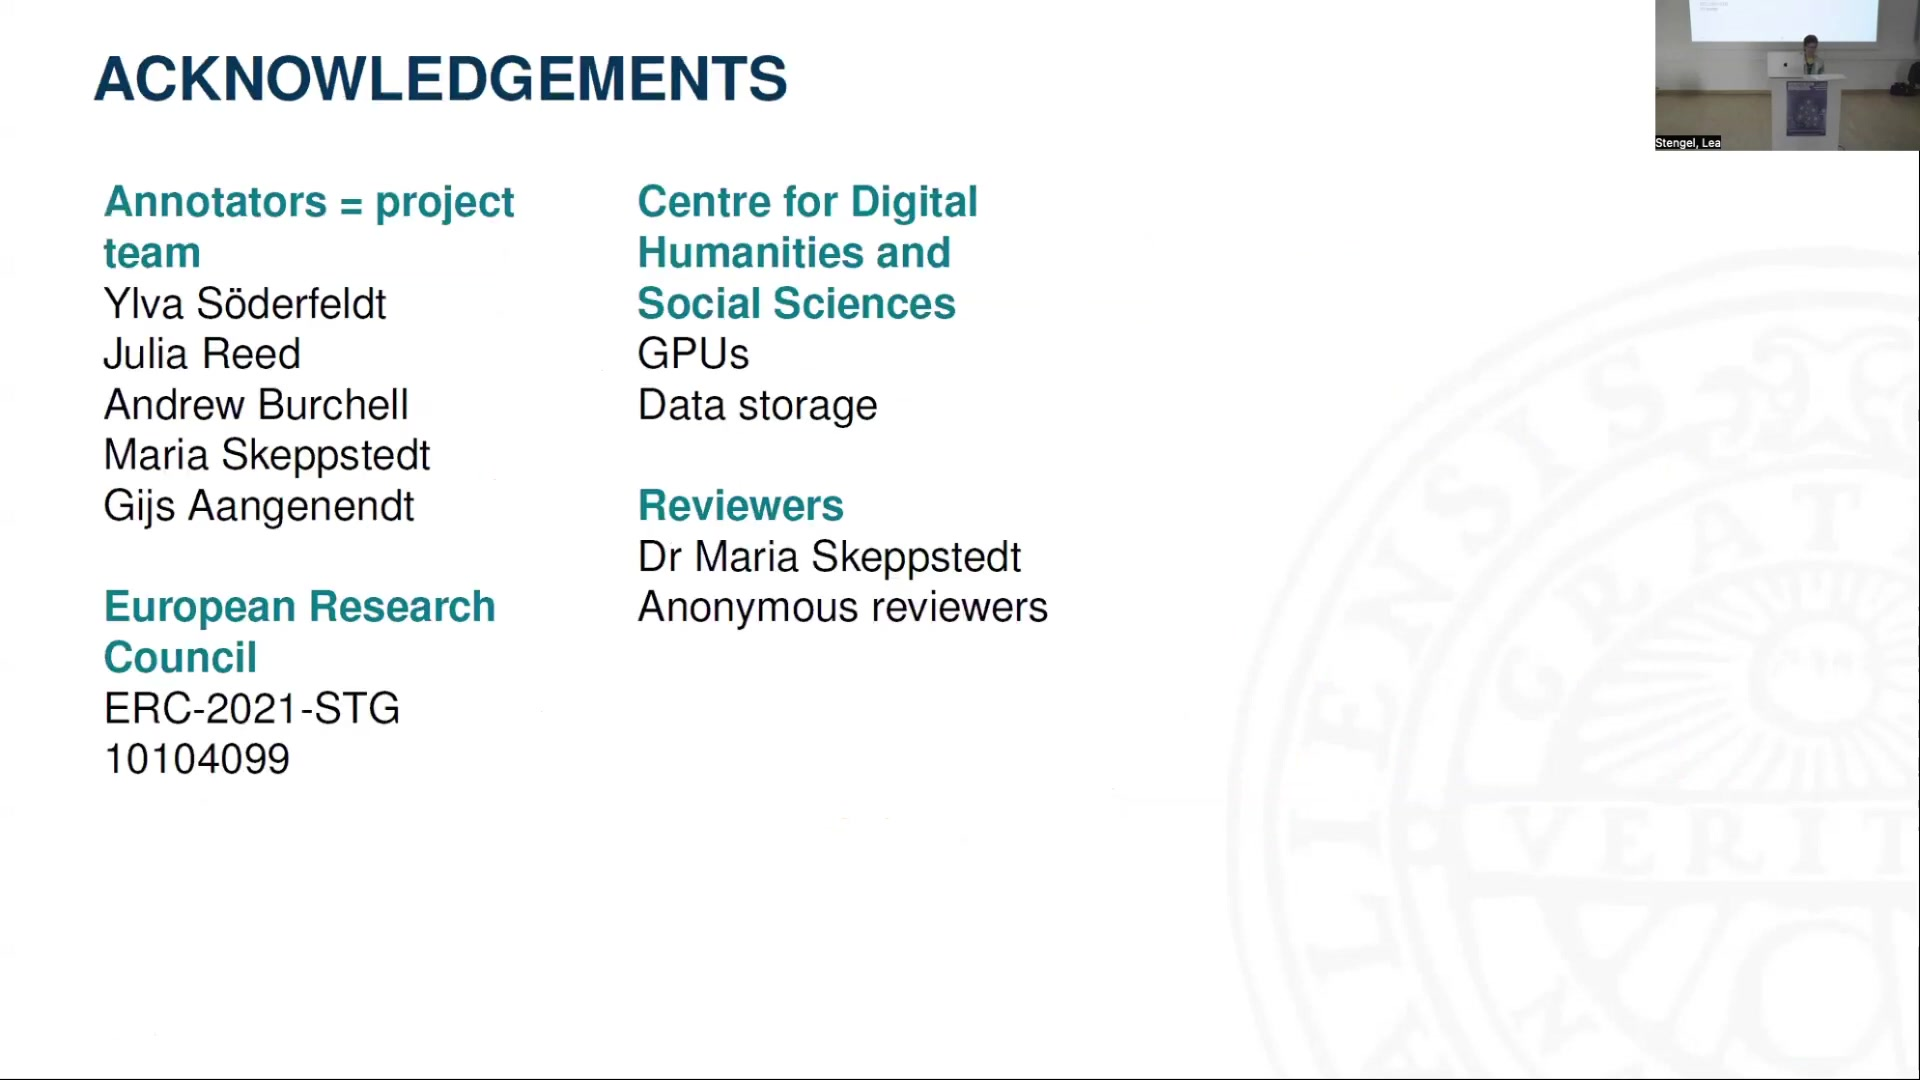
\includegraphics[keepaspectratio]{images/ai-nepi_005_slide_38.jpg}}

}

\caption{Thank you slide with a QR code.}

\end{figure}%

\bookmarksetup{startatroot}

\chapter{---}\label{section-2}

\bookmarksetup{startatroot}

\chapter*{Overview}\label{overview-2}
\addcontentsline{toc}{chapter}{Overview}

\markboth{Overview}{Overview}

The VERITRACE web application, currently in its `alpha' stage of
development, represents an ambitious step towards new research
methodologies. This preliminary version is not yet publicly accessible,
requiring substantial further work; it serves more as a promise of
future capabilities. Central to its current iteration, researchers are
testing a BERT-based Large Language Model (LLM), specifically LaBSE
(Language-agnostic BERT Sentence Embedding), to generate vector
embeddings. These embeddings aim to represent every passage within the
project's extensive textual corpus. However, initial assessments suggest
this model may not ultimately prove sufficient for the complex demands
of the research. The screenshots presented herein offer a glimpse into
the application's design and potential, though they remain a very poor
substitute for direct interaction with the evolving platform.

\section{The VERITRACE Project: Uncovering Ancient Wisdom's
Influence}\label{the-veritrace-project-uncovering-ancient-wisdoms-influence}

The VERITRACE project, a five-year ERC Starting Grant initiative,
embarks on an ambitious journey to trace the intellectual currents
flowing from the early modern `ancient wisdom' tradition into the
burgeoning field of natural philosophy and science of that era. This
tradition manifests in a diverse collection of works, including notable
texts such as the Chaldean Oracles, the Sibylline Oracles, the Orphic
Hymns, and perhaps most famously for historians of chemistry, the Corpus
Hermeticum. These 140 core texts form a `close reading corpus',
providing a focused lens on this influential body of thought.

\begin{figure}[H]

{\centering \pandocbounded{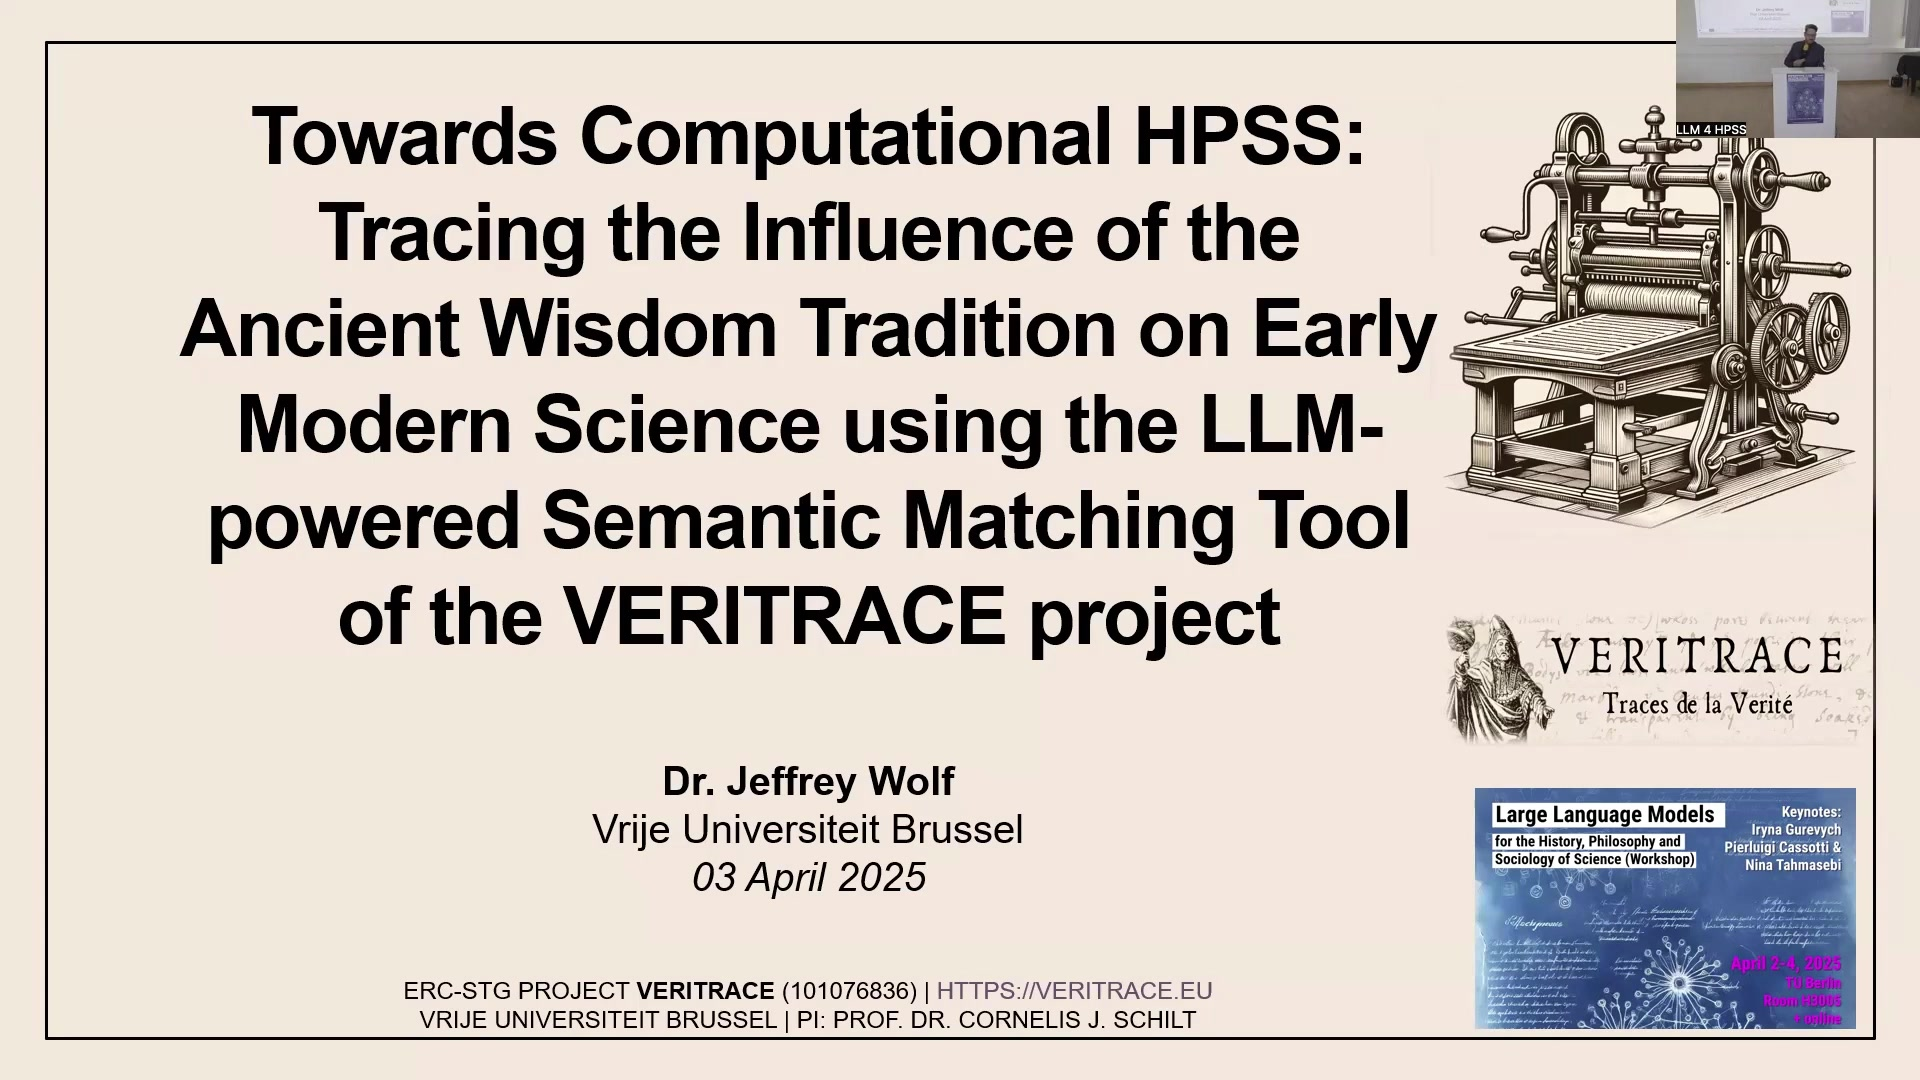
\includegraphics[keepaspectratio]{images/ai-nepi_006_slide_01.jpg}}

}

\caption{Presentation Title Slide illustrating the VERITRACE project's
scope and context.}

\end{figure}%

Historical records confirm the impact of these ancient wisdom texts; for
instance, Newton engaged with the Sibylline Oracles, and Kepler
possessed familiarity with the Corpus Hermeticum. Nevertheless, the
project seeks to delve deeper, aiming to uncover a far broader network
of texts and intellectual connections that interacted with this
tradition. Many of these works, often penned by lesser-known authors,
constitute what one scholar has termed `the great unread', frequently
overlooked by historians due to their sheer volume and obscurity.
Consequently, VERITRACE focuses on bringing these neglected sources to
light.

\section{Advancing Computational History, Philosophy, and Sociology of
Science
(HPSS)}\label{advancing-computational-history-philosophy-and-sociology-of-science-hpss}

To address its core research questions, the VERITRACE project pioneers
large-scale, multilingual exploration within the domain of computational
History, Philosophy, and Sociology of Science (HPSS). The team develops
tools not only for conventional keyword searching but also for the
sophisticated identification of textual reuse. This encompasses both
direct, lexical quotation---instances where authors use verbatim
material from other works, perhaps without explicit citation---and more
subtle, indirect influences. Such indirect reuse might involve
paraphrase or allusions that, whilst not direct copies, would have been
recognisable to contemporary readers as originating from sources like
the Corpus Hermeticum.

\begin{figure}[H]

{\centering \pandocbounded{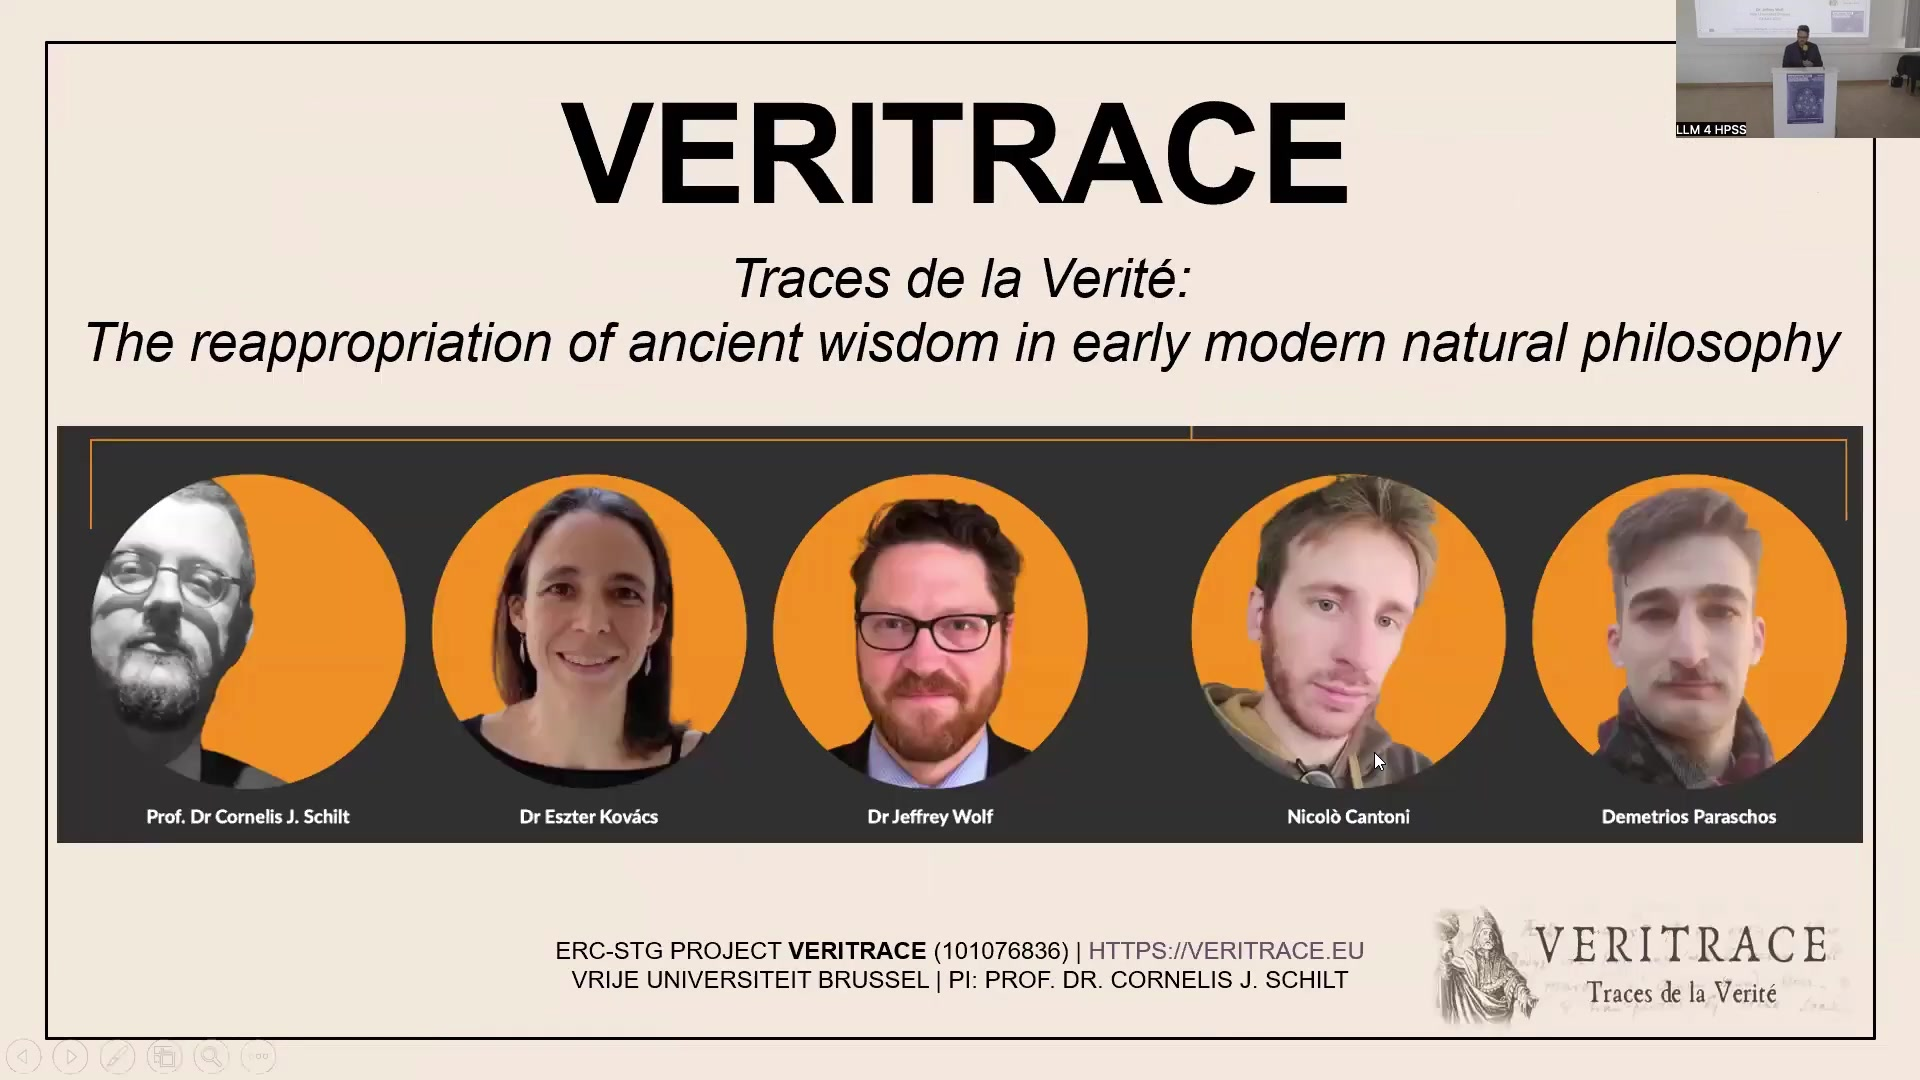
\includegraphics[keepaspectratio]{images/ai-nepi_006_slide_02.jpg}}

}

\caption{The VERITRACE project team and its mission statement.}

\end{figure}%

Effectively, the project endeavours to construct an `early modern
plagiarism detector' capable of navigating a vast, multilingual corpus.
Beyond identifying direct and indirect textual linkages, a primary
objective is to uncover previously ignored networks of texts, passages,
themes, topics, and authors. Through this comprehensive analytical
approach, researchers anticipate the emergence of new patterns and
insights into the intellectual history and philosophy of science.

\begin{figure}[H]

{\centering \pandocbounded{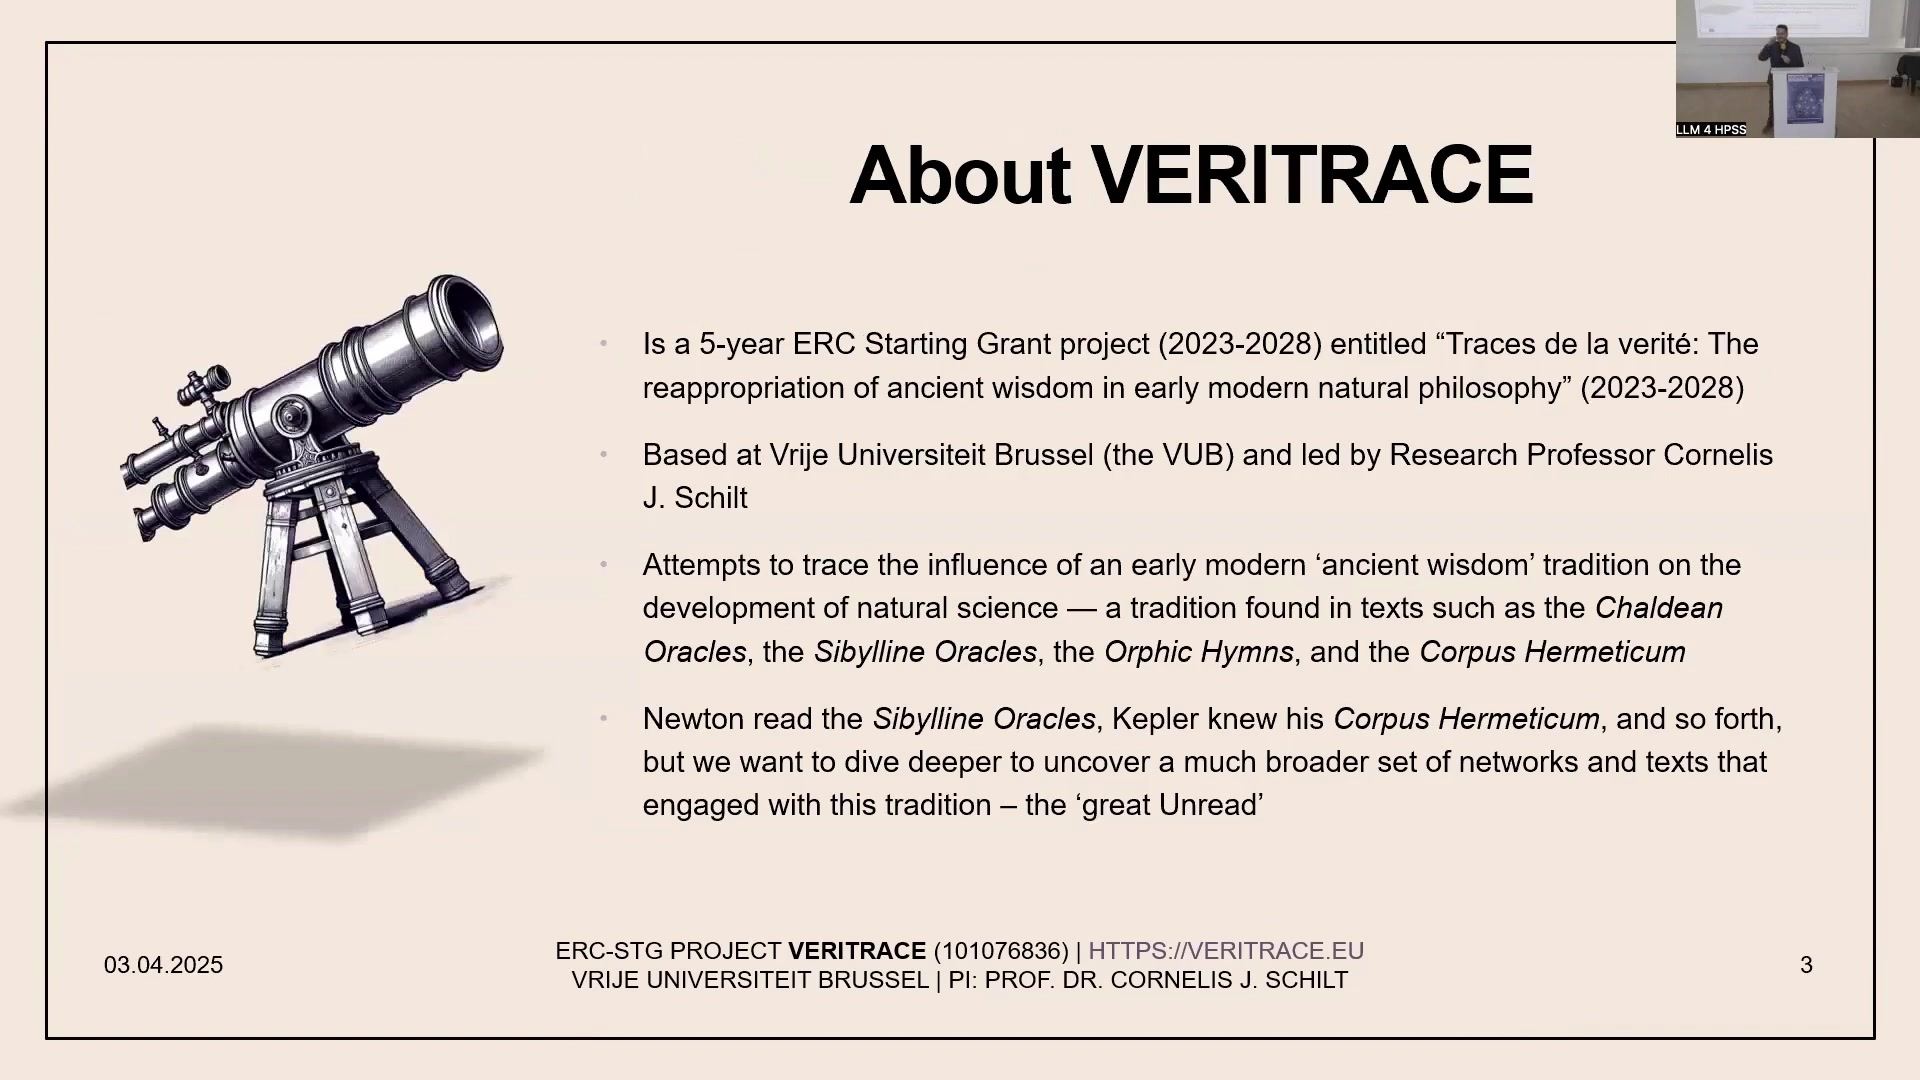
\includegraphics[keepaspectratio]{images/ai-nepi_006_slide_03.jpg}}

}

\caption{Key objectives of the VERITRACE project in computational HPSS.}

\end{figure}%

\section{Navigating a Vast Multilingual
Corpus}\label{navigating-a-vast-multilingual-corpus}

The foundation of this investigation rests upon a large, diverse, and
multilingual dataset, focusing exclusively on printed books and texts,
thereby excluding handwritten materials from its current scope. This
corpus draws from three primary data sources and encompasses works in at
least six different languages, published over approximately two
centuries. The chronological parameters span from 1540, chosen for
specific historical reasons, to 1728, shortly after Newton's death.

Key data repositories include:

\begin{itemize}
\item
  Early English Books Online (EEBO)
\item
  Gallica, the digital library of the French National Library
\item
  The Bavarian State Library, which constitutes the largest single
  source
\end{itemize}

Collectively, these sources contribute to a corpus of roughly 430,000
books. State-of-the-art digital techniques are employed to analyse this
extensive collection of early modern texts.

\begin{figure}[H]

{\centering \pandocbounded{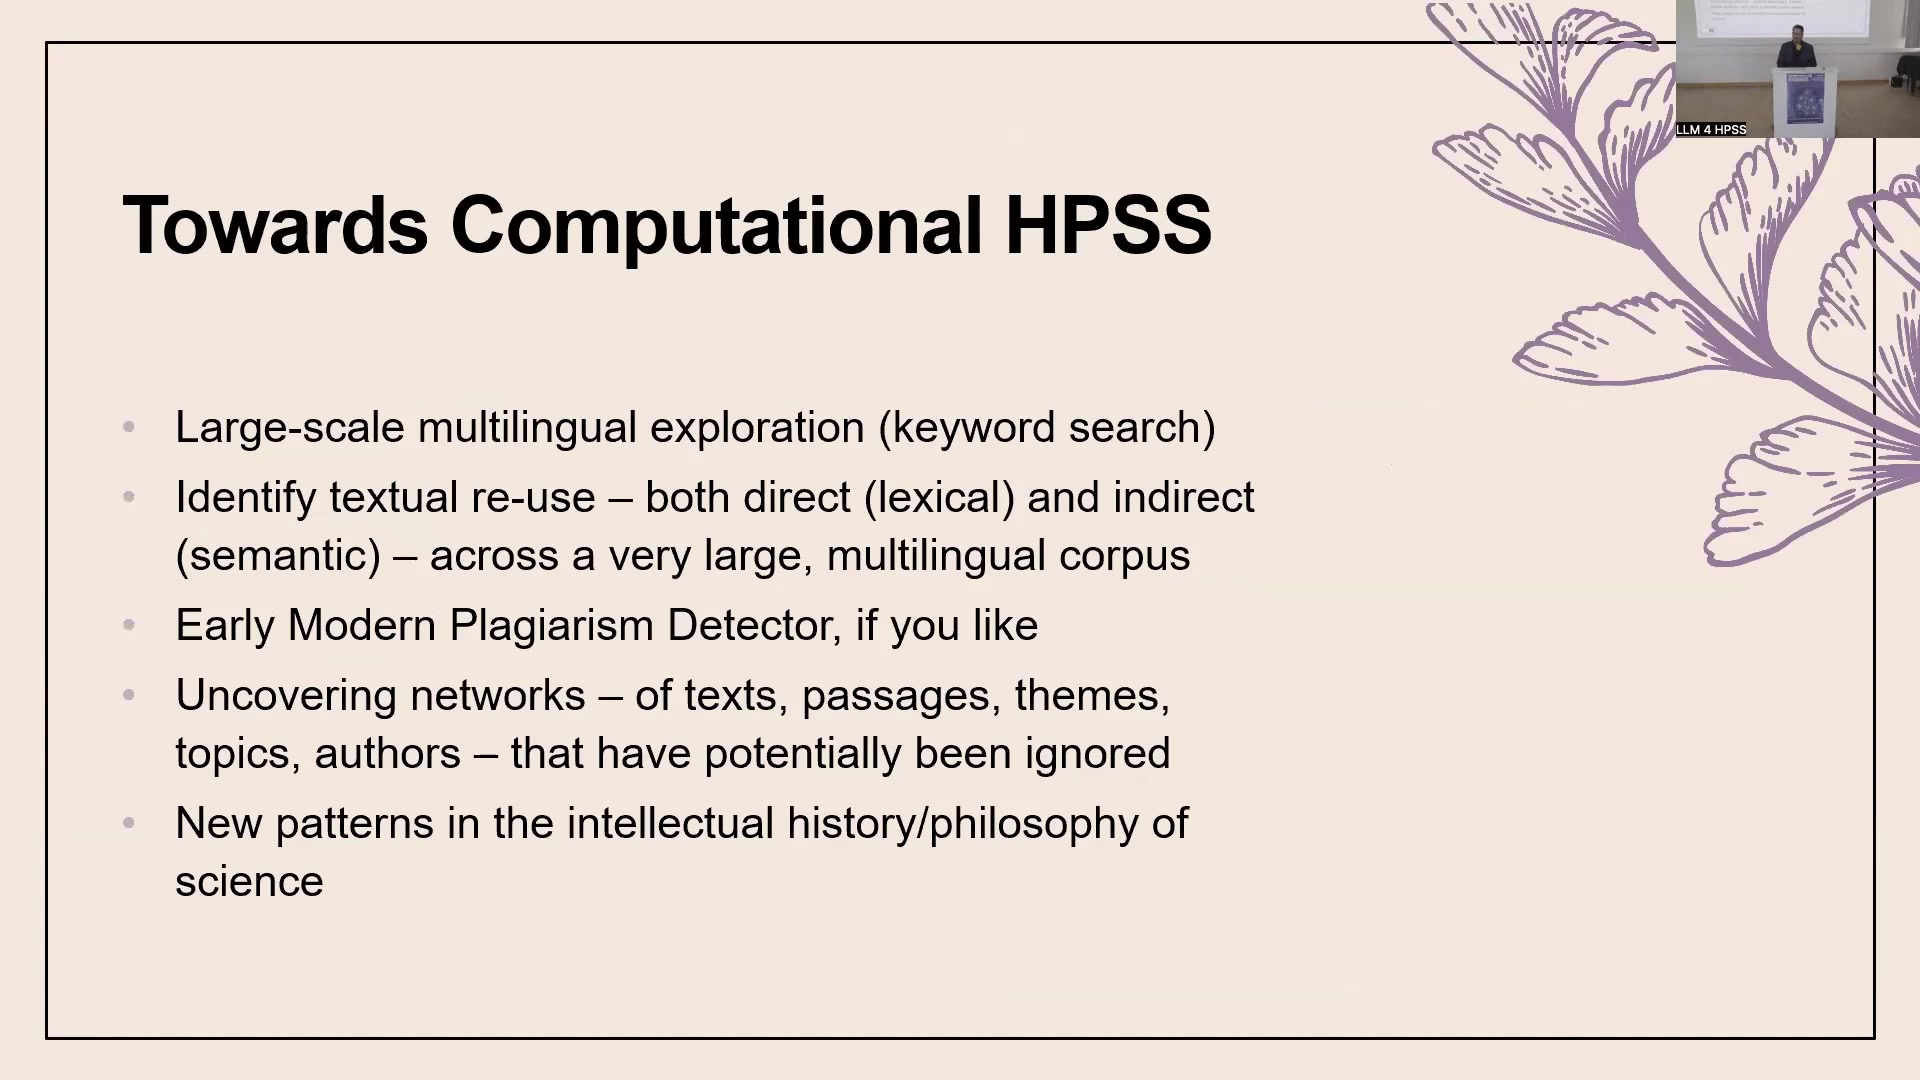
\includegraphics[keepaspectratio]{images/ai-nepi_006_slide_04.jpg}}

}

\caption{Overview of the large, diverse, and multilingual dataset used
by VERITRACE.}

\end{figure}%

\section{Core Challenges and the Role of Large Language
Models}\label{core-challenges-and-the-role-of-large-language-models}

Several core challenges are inherent in a project of this scale and
complexity. Variable Optical Character Recognition (OCR) quality
presents a significant hurdle. The textual data, supplied directly by
libraries in raw formats such as XML, HOCR, or even HTML files, often
lacks ground truth page images. This variability in OCR accuracy
inevitably affects all downstream processing and analytical tasks.
Managing early modern typography and semantics across at least six
languages introduces further complexities. Furthermore, the sheer volume
of data---hundreds of thousands of texts printed across Europe over
nearly 200 years---demands robust computational strategies.

Large Language Models (LLMs) play a crucial role in addressing these
challenges. On the decoder side, GPT-based LLMs assist in enriching and
cleaning metadata, acting as `judges' in this process. Whilst this
application holds considerable interest, the current focus shifts
towards the encoder side. Here, BERT-based LLMs generate embeddings to
encode the semantic meaning of sentences and short passages (groups of
sentences) within the textual corpus. This encoding is fundamental to
the project's semantic matching capabilities.

\section{Employing LLMs as Judges for Metadata
Enrichment}\label{employing-llms-as-judges-for-metadata-enrichment}

One specific, albeit challenging, application of LLMs within VERITRACE
involves their use as `judges' to enrich metadata. The basic motivation
stems from the desire to map records from high-quality external sources,
such as the Universal Short Title Catalogue (USTC), onto the project's
own records. Successful mapping creates enriched metadata, less likely
to require extensive manual cleaning.

\begin{figure}[H]

{\centering \pandocbounded{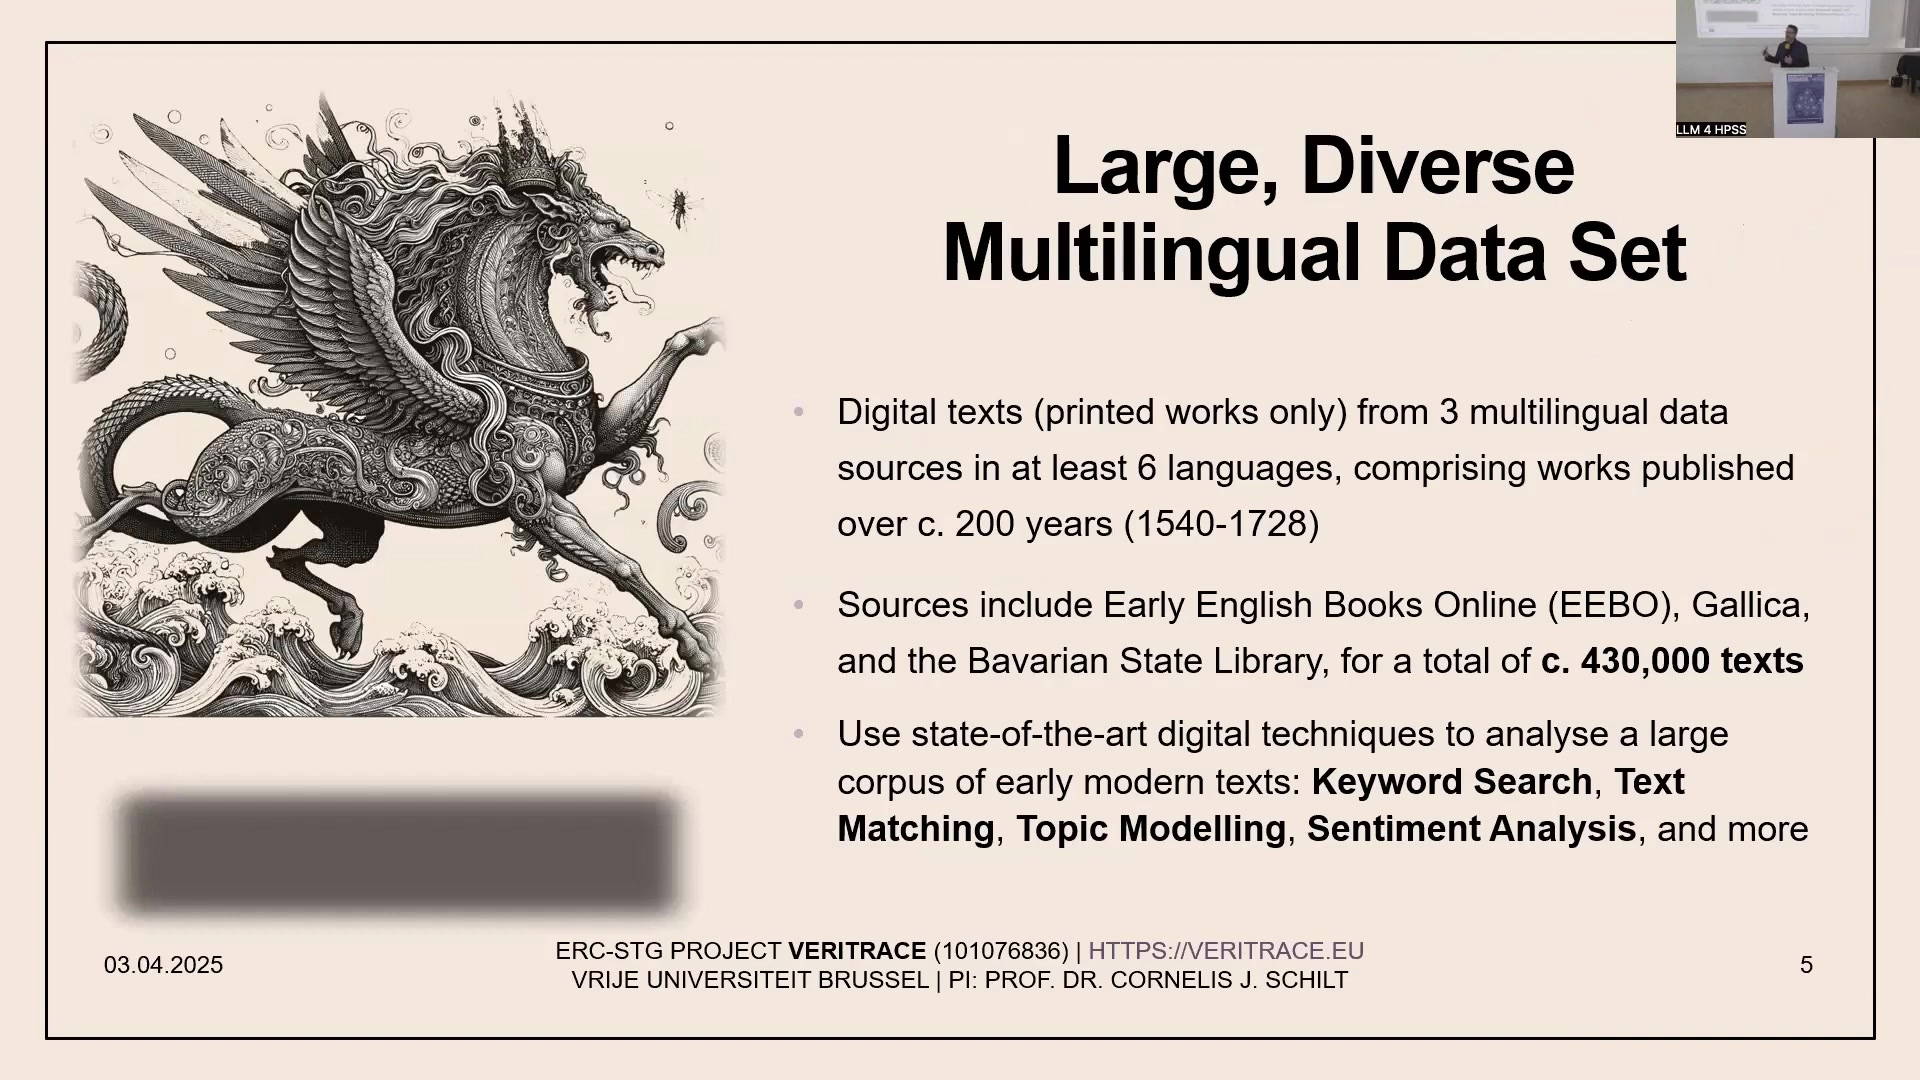
\includegraphics[keepaspectratio]{images/ai-nepi_006_slide_05.jpg}}

}

\caption{Case study overview of using LLMs as judges to enrich VERITRACE
metadata.}

\end{figure}%

Whilst some mapping can be automated using external identifiers, many
records lack such straightforward connections. Compounding this, much of
the project's internal data has not yet undergone cleaning, making
matching a non-trivial task. The manual comparison of bibliographic
metadata---assessing pairs of records to determine if they represent the
same underlying printed text---is exceedingly tedious. Team members
faced the prospect of reviewing tens of thousands of such pairs,
highlighting the need for an automated solution.

\subsection{Initial Attempts and Emerging
Hurdles}\label{initial-attempts-and-emerging-hurdles}

To address this, researchers are exploring a panel, or `bench', of LLMs.
Extensive prompt guidelines direct these models to evaluate potential
matches, which are initially generated via fuzzy matching algorithms.
The LLMs provide yes/no decisions along with reasoning for why a pair of
records may or may not represent the same underlying text.

\begin{figure}[H]

{\centering \pandocbounded{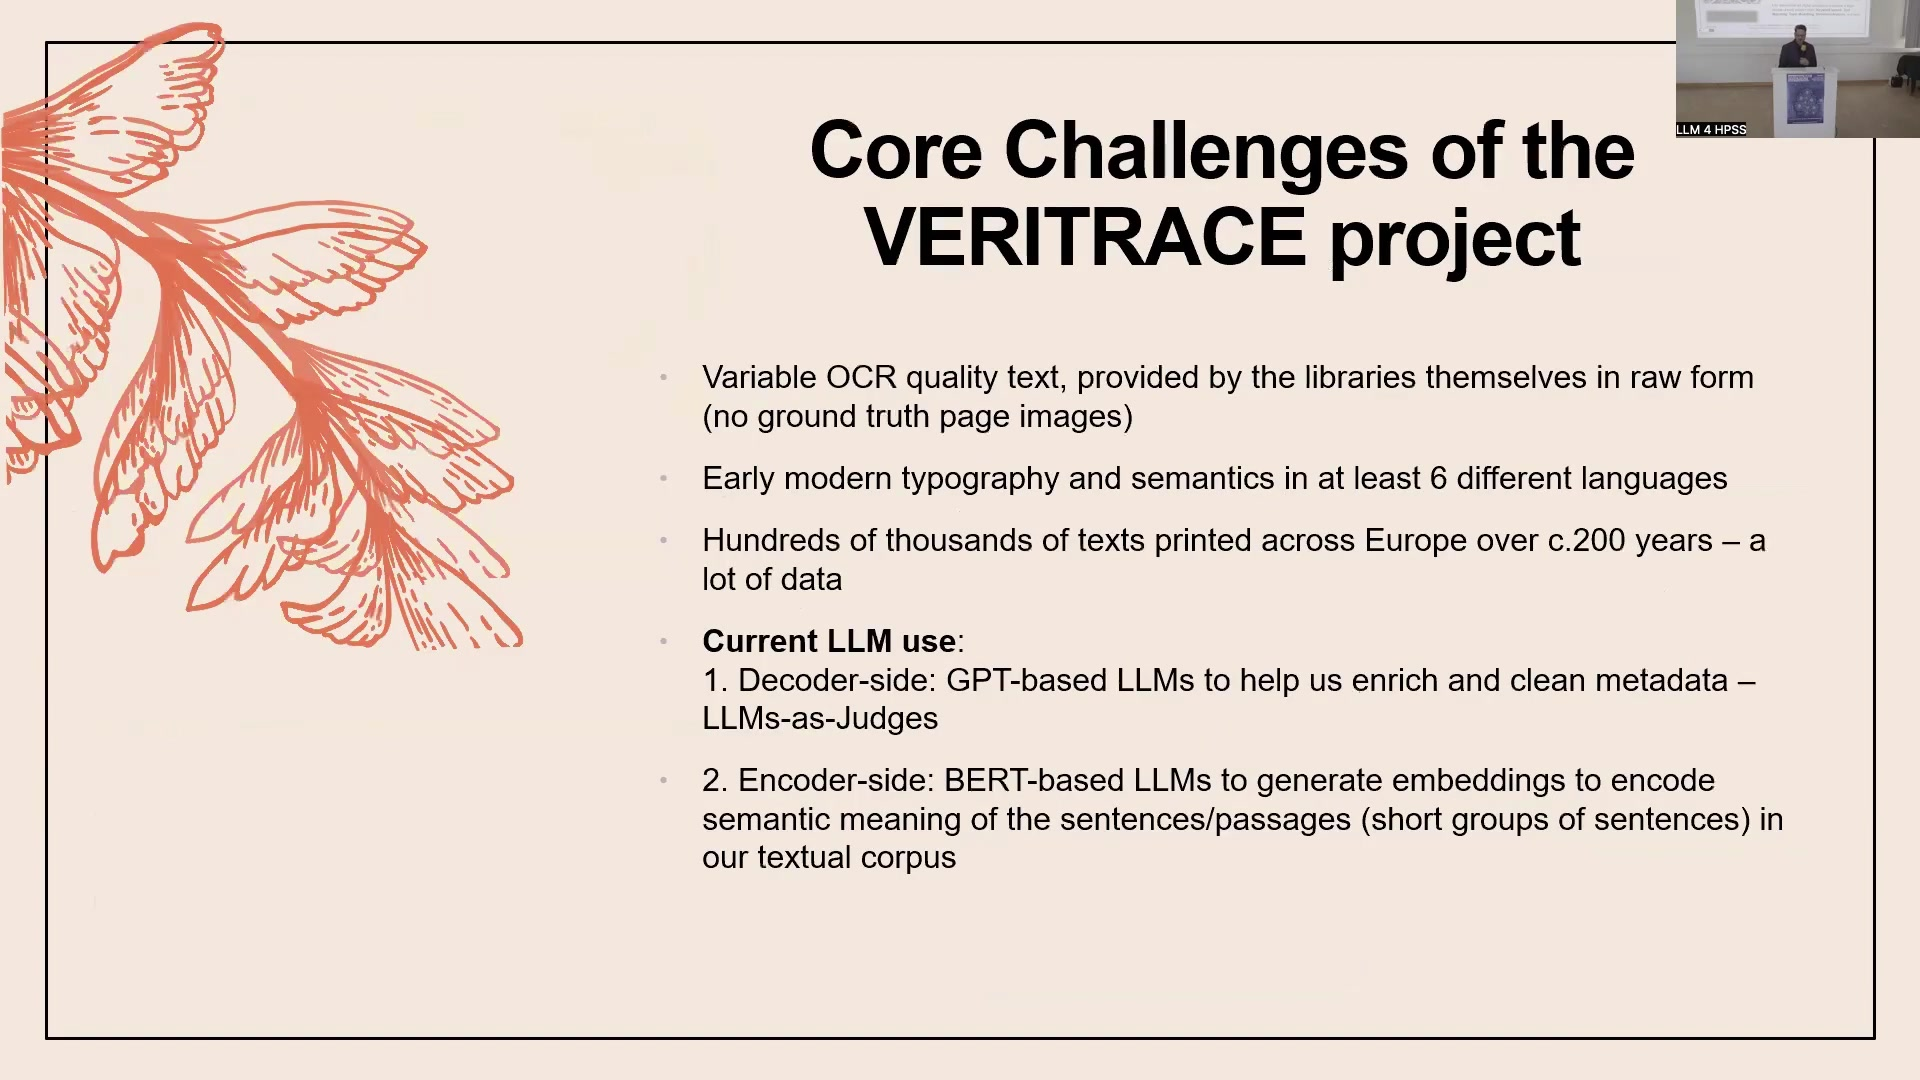
\includegraphics[keepaspectratio]{images/ai-nepi_006_slide_06.jpg}}

}

\caption{Example of metadata comparison for LLM judging.}

\end{figure}%

This endeavour remains a work in progress. A major current challenge is
the prevalence of hallucinations in the output from the open-source
models (e.g., Llama-based) currently under evaluation. Attempts to
mitigate this by requesting more structured output, paradoxically, often
lead to more generic and less helpful responses, particularly in the
reasoning provided by the models. Achieving the right balance in
prompting to elicit accurate and insightful judgments is an ongoing
refinement process. Despite these initial difficulties, the potential
for LLMs to save considerable time in metadata enrichment remains
significant, and further investigation is warranted.

\begin{figure}[H]

{\centering \pandocbounded{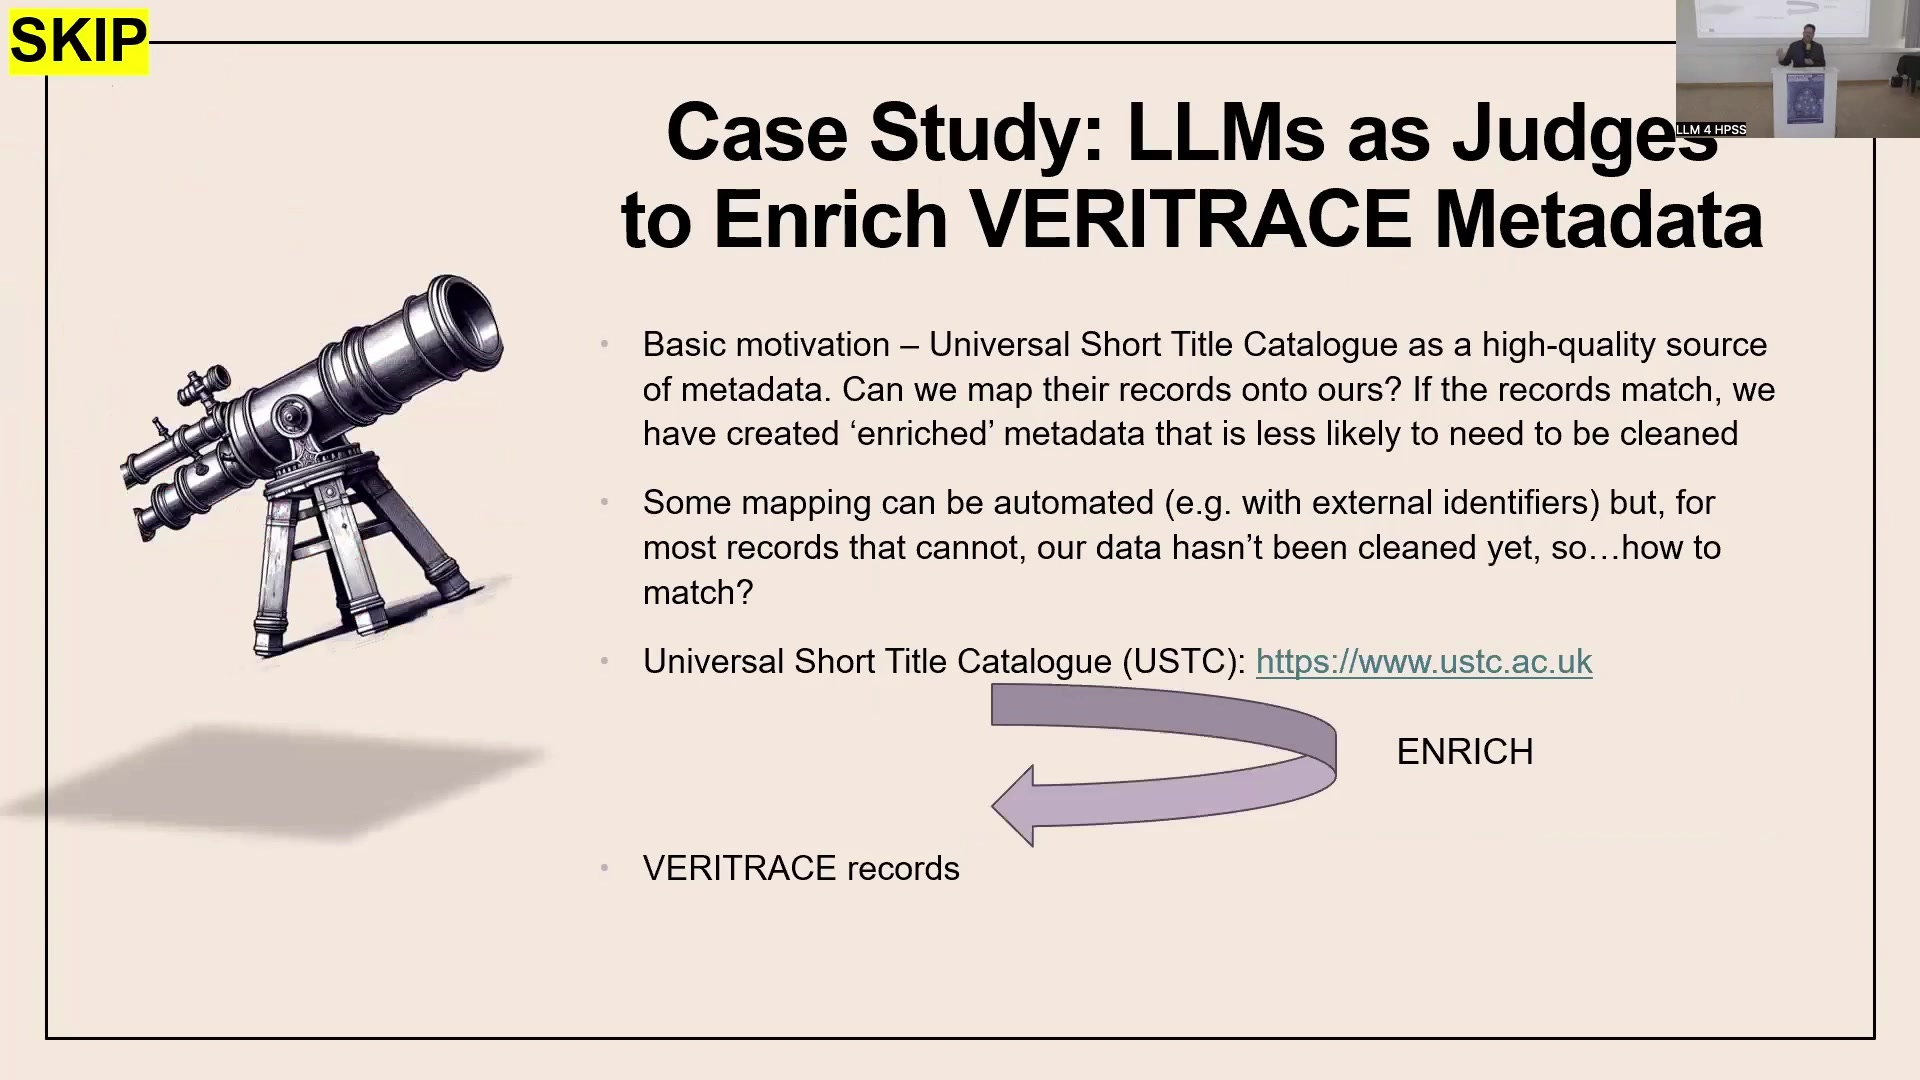
\includegraphics[keepaspectratio]{images/ai-nepi_006_slide_07.jpg}}

}

\caption{Example of prompt guidelines and LLM output for metadata
matching.}

\end{figure}%

\section{Introducing the VERITRACE Web
Application}\label{introducing-the-veritrace-web-application}

The VERITRACE web application serves as the primary interface for
exploring the project's data and analytical tools. This platform is
exceptionally new; indeed, its introduction here marks its first public
discussion, preceding even internal team dissemination. As an `alpha'
version, it is not yet publicly available and remains under active
development on a local machine, with screenshots offering a preliminary
view. It functions more as a demonstration of the project's aspirations
than a finalised product.

\begin{figure}[H]

{\centering \pandocbounded{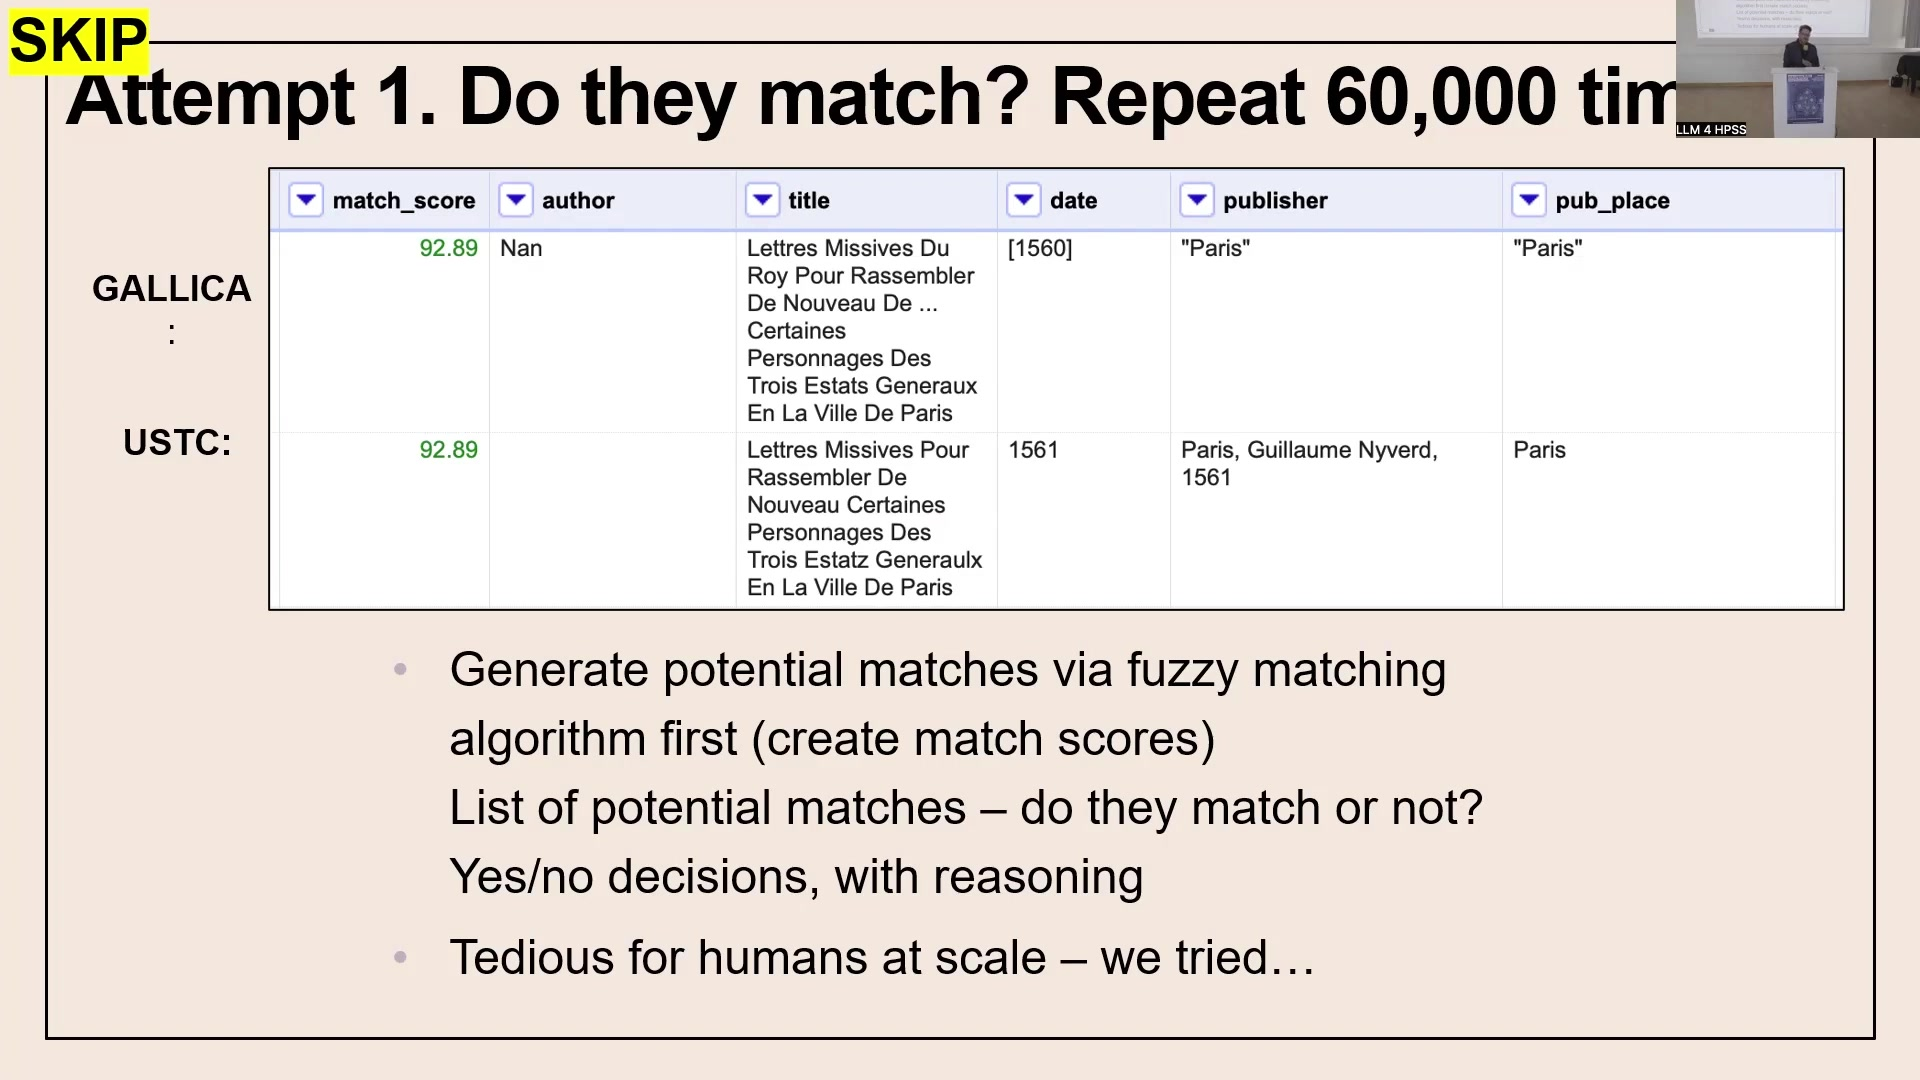
\includegraphics[keepaspectratio]{images/ai-nepi_006_slide_08.jpg}}

}

\caption{Overview of the VERITRACE Web Application's alpha version.}

\end{figure}%

Currently, testing involves a BERT-based LLM (LaBSE) to generate vector
embeddings for every passage in the corpus. However, early indications
suggest this model may not possess the requisite sophistication for the
project's ultimate goals, particularly for nuanced semantic matching.
The application's development continues, with these initial explorations
informing future refinements.

\section{The Data Processing
Backbone}\label{the-data-processing-backbone}

Transforming raw textual data from library sources into a queryable
format within an Elasticsearch database---the backend of the web
application---involves an intricate data processing pipeline. This
multi-stage process is far from a simple button-push operation. Numerous
steps are essential to prepare the data for analysis.

\begin{figure}[H]

{\centering \pandocbounded{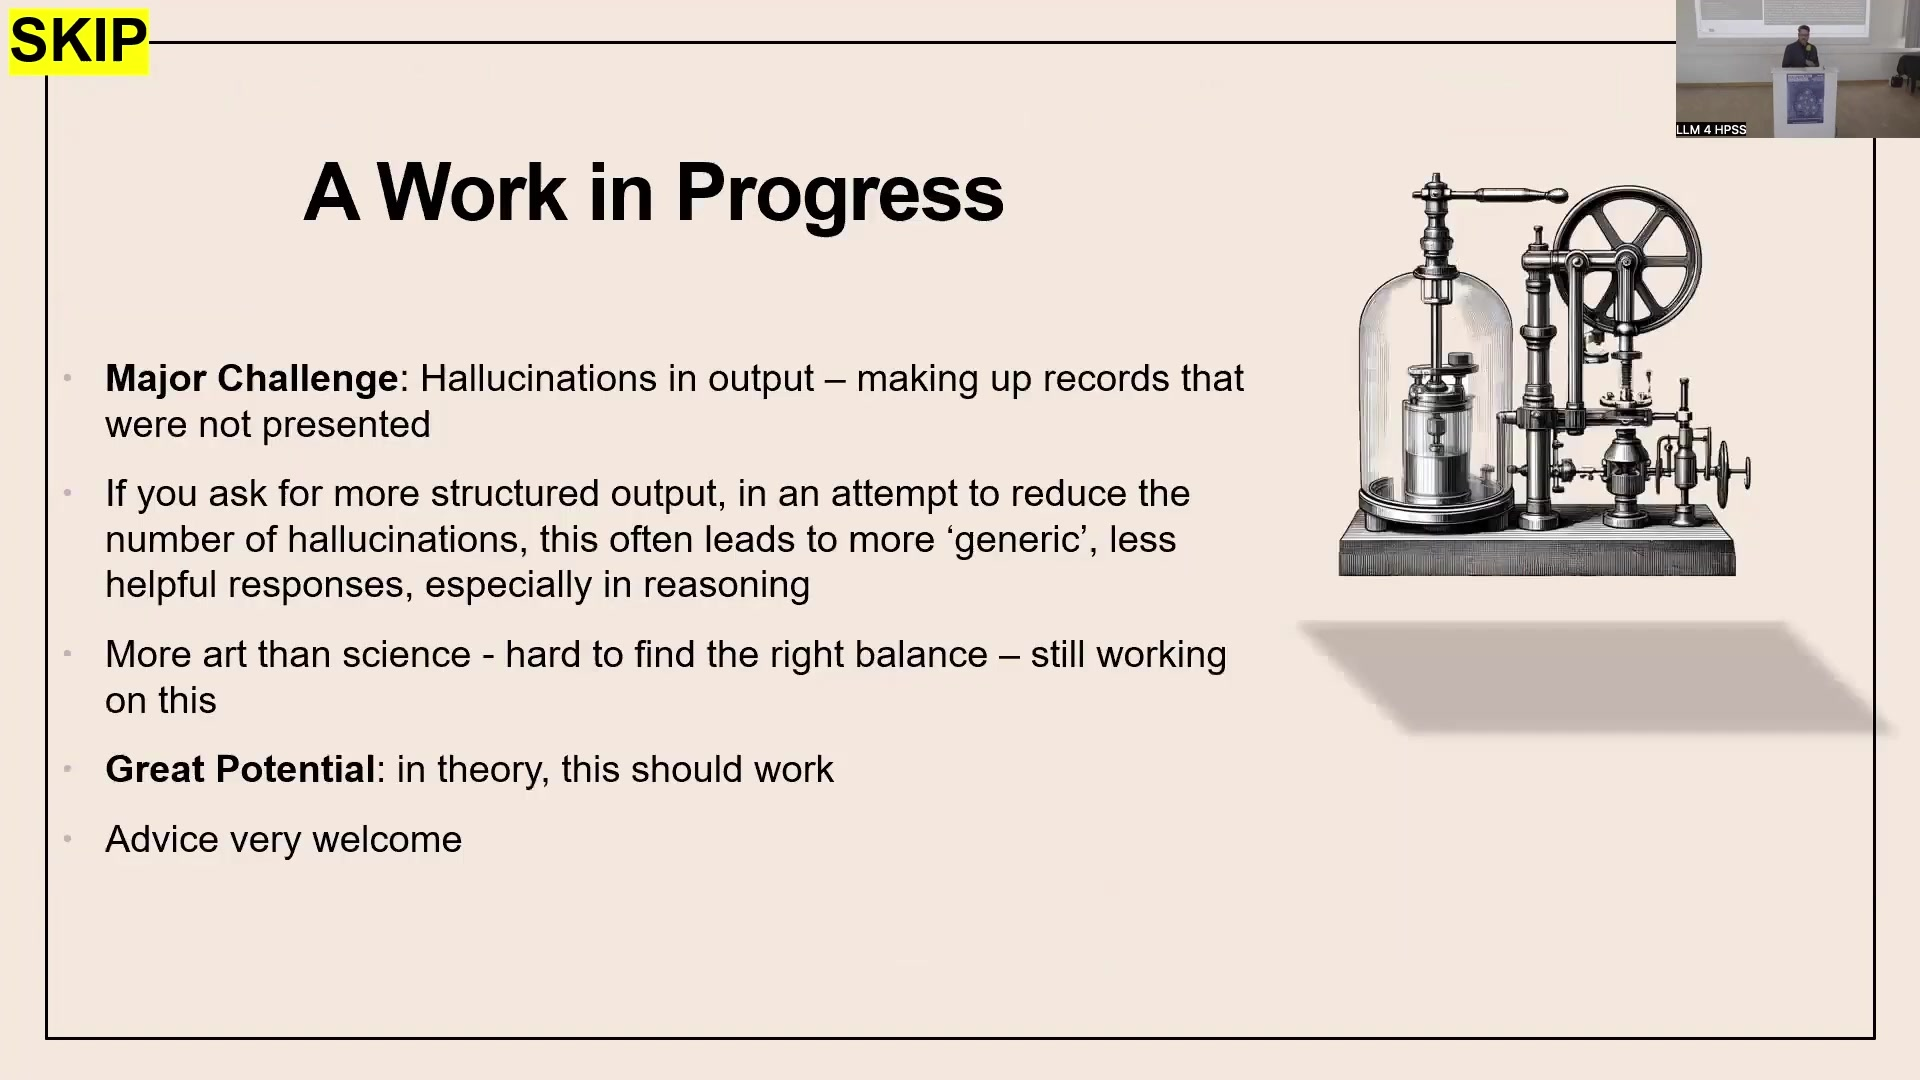
\includegraphics[keepaspectratio]{images/ai-nepi_006_slide_09.jpg}}

}

\caption{Diagram of the VERITRACE data processing pipeline dashboard and
stages.}

\end{figure}%

These steps include:

\begin{itemize}
\item
  Extracting text into manageable files.
\item
  Generating mappings of all character positions.
\item
  Segmenting texts into meaningful units.
\item
  Assessing OCR quality.
\end{itemize}

Each of these fifteen stages requires careful optimisation. The
generation of embeddings, crucial for semantic analysis, occurs near the
end of this complex pipeline. Significant background work underpins the
functionality accessible through the web interface.

\section{Exploring the VERITRACE Corpus: Statistics and
Metadata}\label{exploring-the-veritrace-corpus-statistics-and-metadata}

The VERITRACE web application offers several modules for interacting
with the corpus. The `Explore' section, for instance, provides users
with comprehensive statistics about the dataset, drawn directly from a
MongoDB database. At present, this encompasses 427,305 metadata records
describing the books within the collection. This area allows researchers
to gain an overview of the corpus's composition, including language
distributions, data sources, publication decades, and prominent
publication places.

\begin{figure}[H]

{\centering \pandocbounded{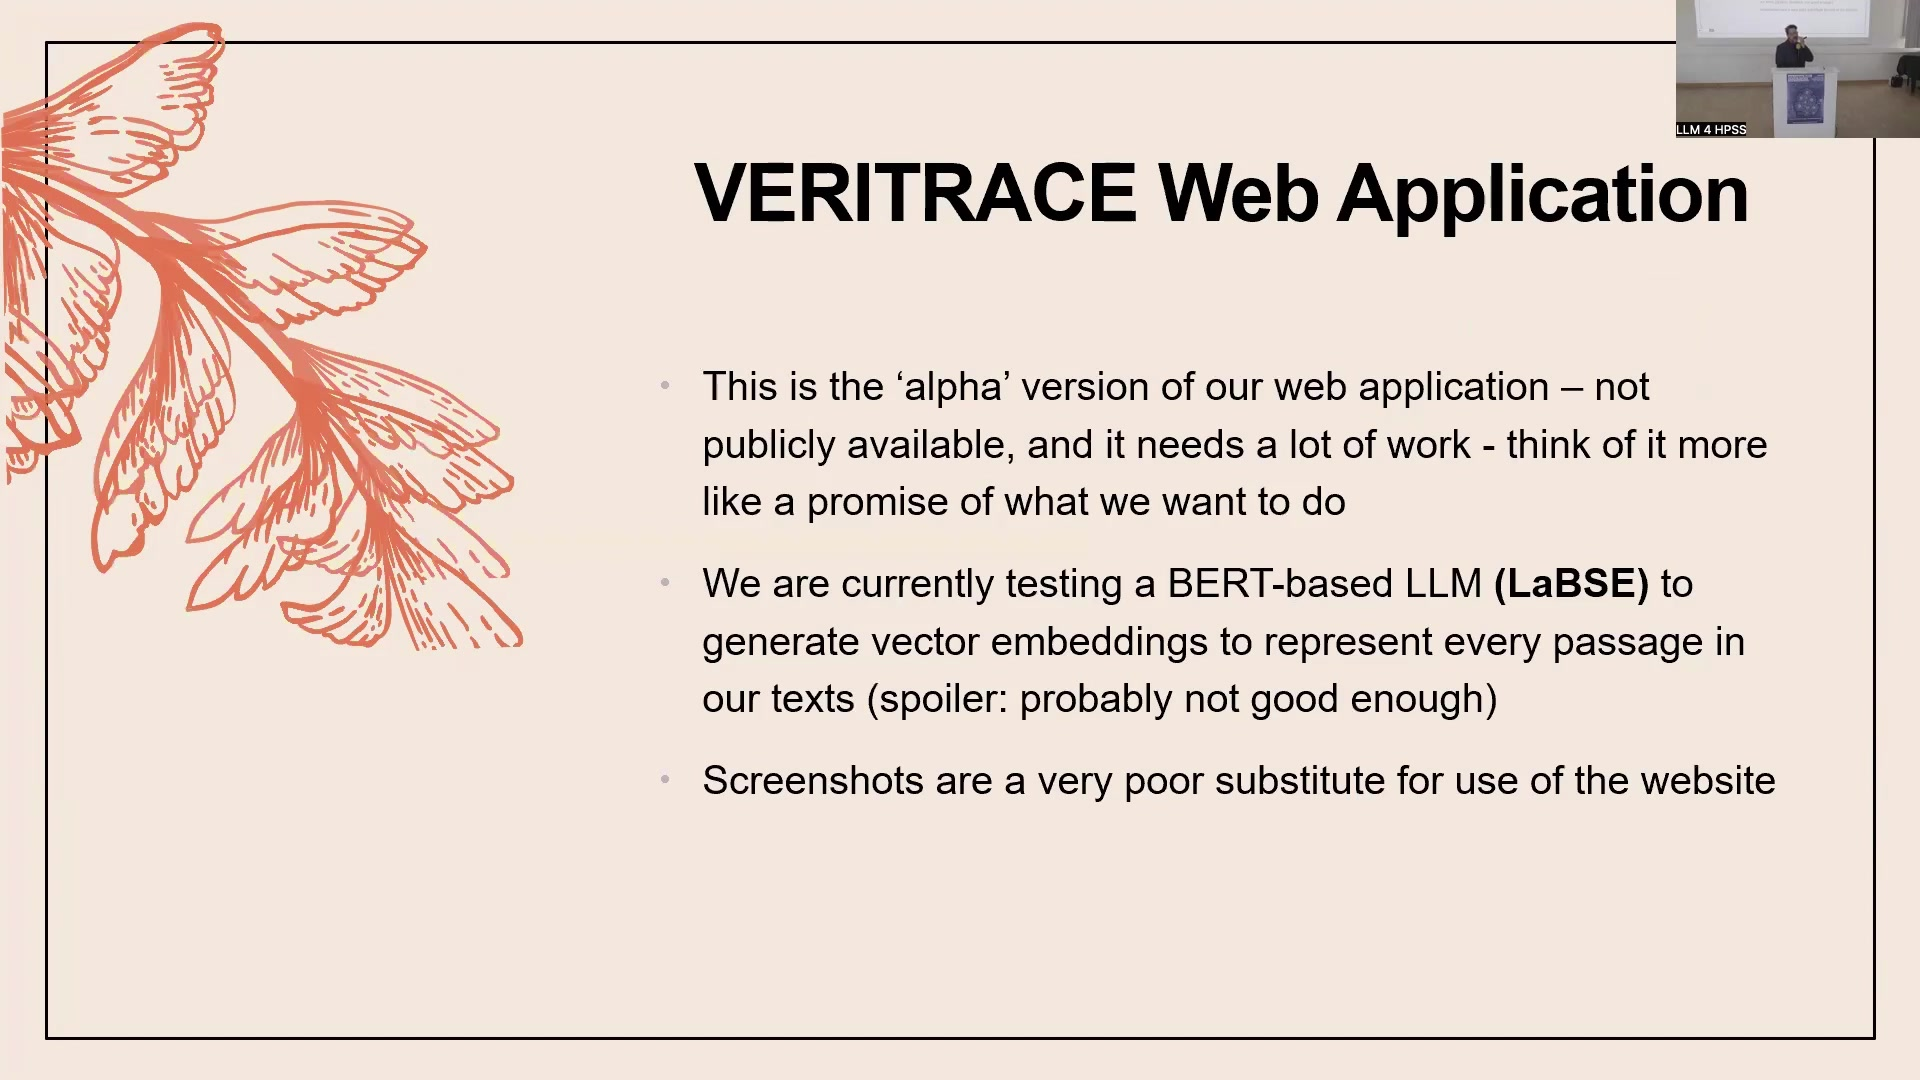
\includegraphics[keepaspectratio]{images/ai-nepi_006_slide_10.jpg}}

}

\caption{The VERITRACE `Explore' interface showing corpus statistics.}

\end{figure}%

Beyond aggregate statistics, a `Metadata Explorer' enables users to
browse and inspect the rich metadata associated with each text. A key
feature here is detailed language information. Language identification
algorithms operate on every text, down to segments of approximately 50
characters. This granularity is vital because many early modern texts
are multilingual, often containing sections in Greek or other languages
alongside the primary Latin, for example. The system identifies these
languages and their proportions within each document---such as a text
being 15\% Greek and 85\% Latin---classifying them as `substantively
multilingual'.

Furthermore, the system attempts to assess OCR quality on a page-by-page
basis. This is a challenging task without access to ground truth page
images, relying instead on analysis of the raw text. Nevertheless,
providing page-level quality assessments, rather than a single score for
an entire book, offers more nuanced information for researchers. The
efficacy of this OCR assessment method continues to be evaluated.

\begin{figure}[H]

{\centering \pandocbounded{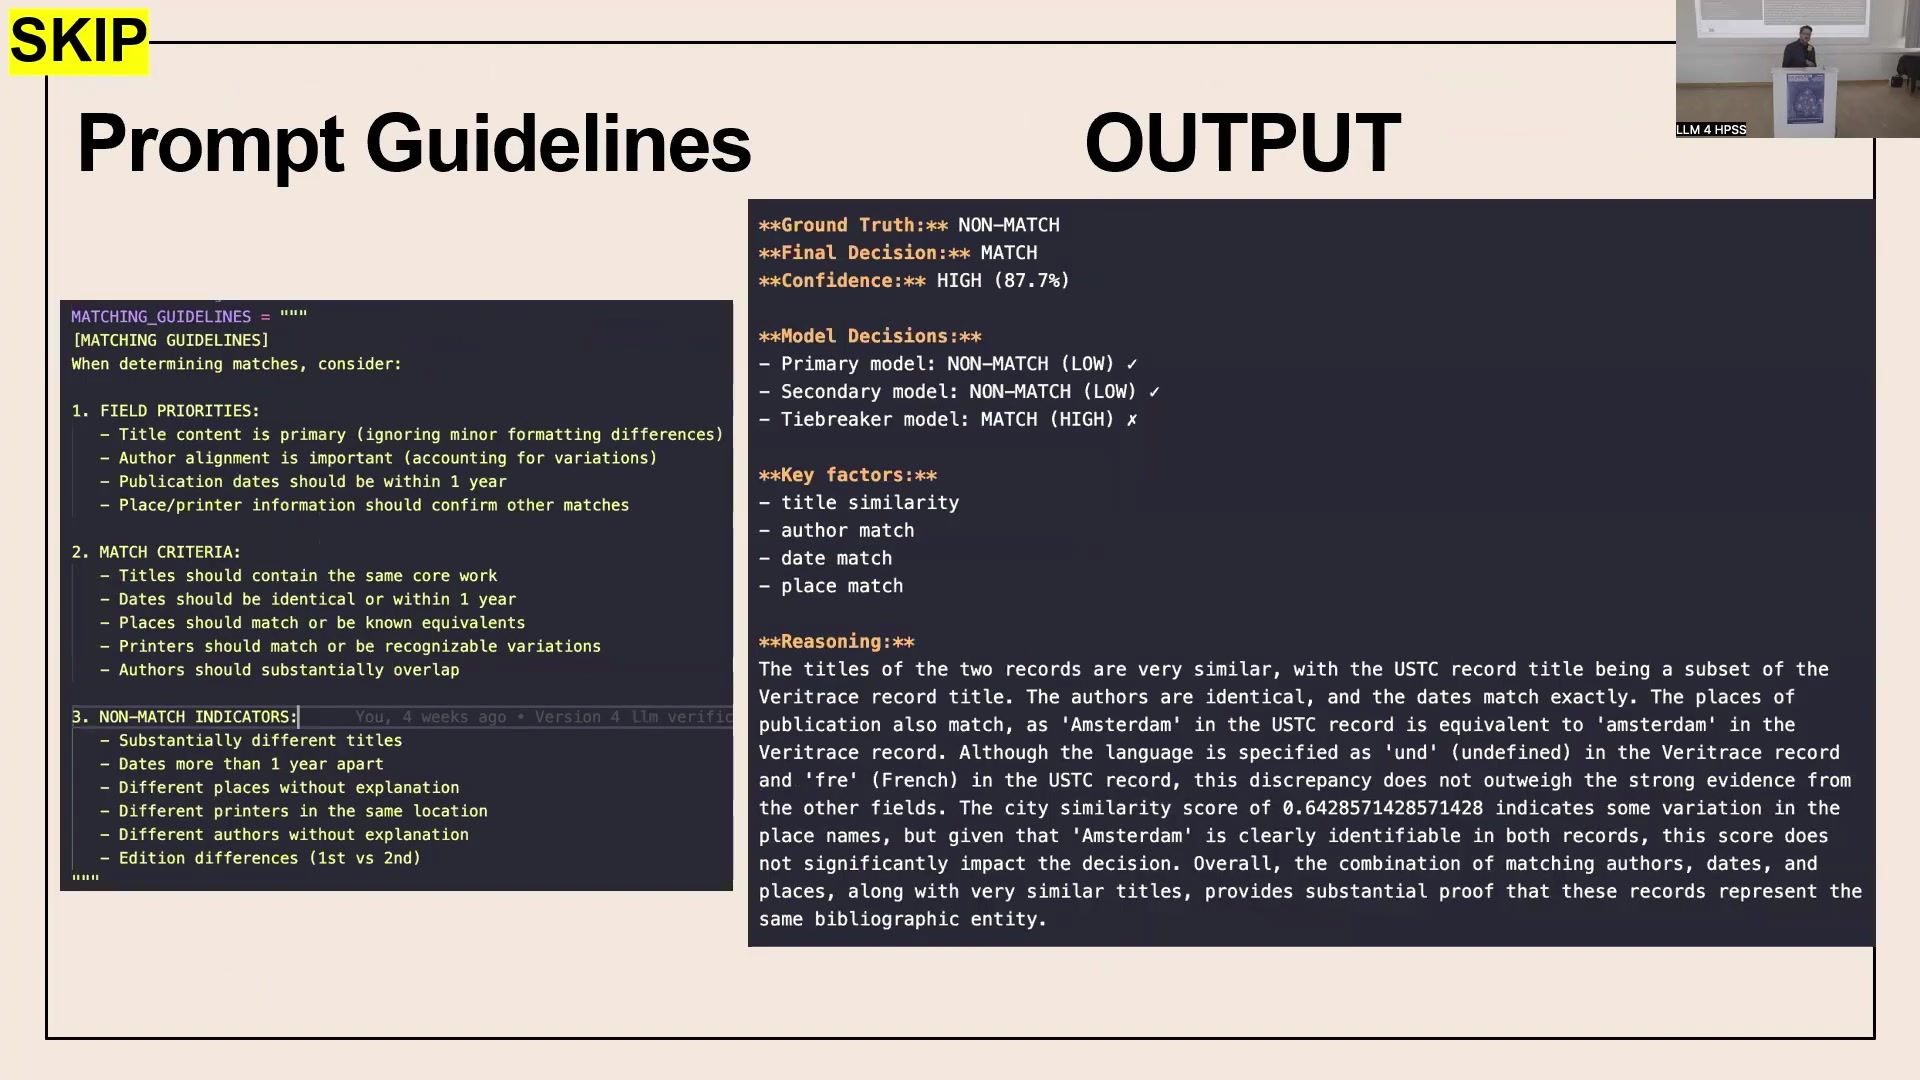
\includegraphics[keepaspectratio]{images/ai-nepi_006_slide_11.jpg}}

}

\caption{The VERITRACE `Metadata Explorer' interface displaying detailed
record information.}

\end{figure}%

\section{Search, Analysis, and Reading: Tools for Scholarly
Inquiry}\label{search-analysis-and-reading-tools-for-scholarly-inquiry}

For many scholars, the `Search' function will likely be the initial
point of engagement. The web application supports standard keyword
searches across the corpus. Even with a prototype dataset of only 132
files (rather than the full 430,000), the Elasticsearch index already
occupies 15 gigabytes, hinting at the terabytes of data the full system
will manage. A simple search for ``Hermes'' in this prototype, for
example, might yield 22 documents with 332 total matches.

\begin{figure}[H]

{\centering \pandocbounded{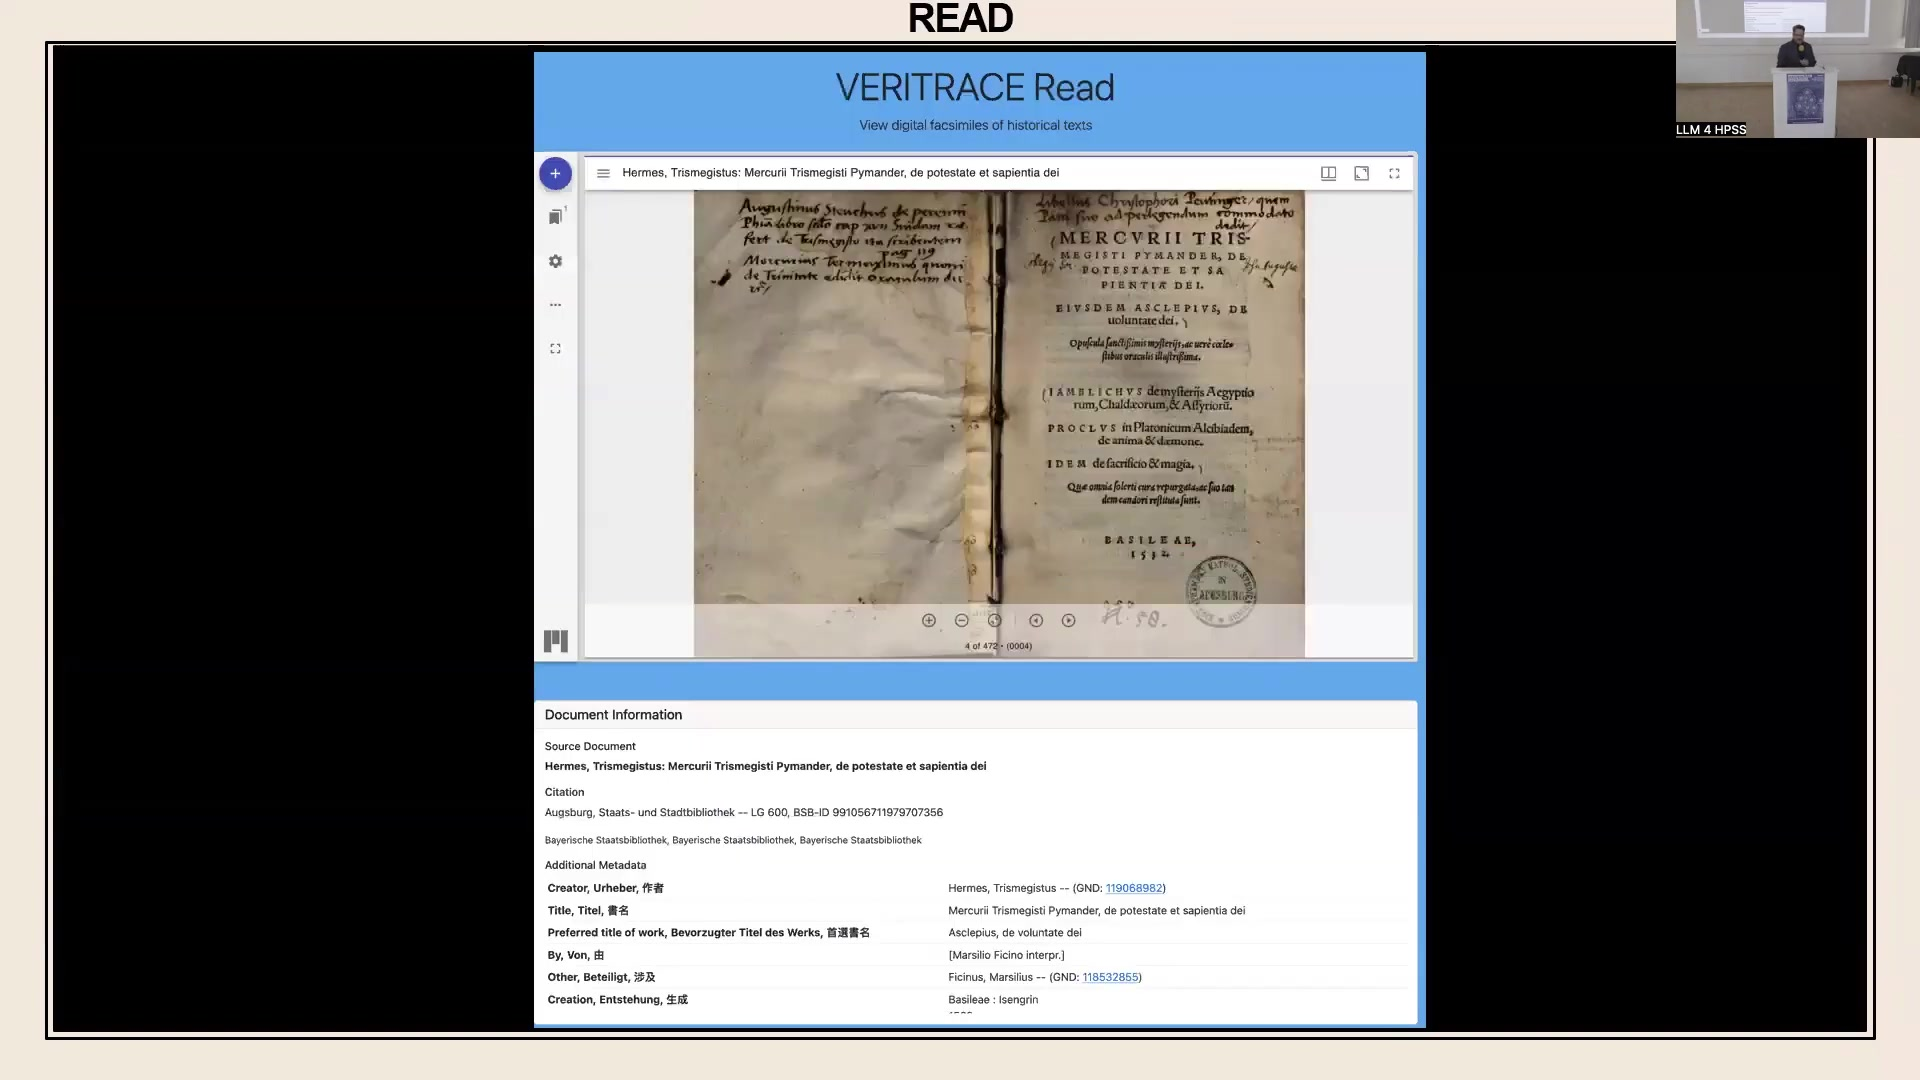
\includegraphics[keepaspectratio]{images/ai-nepi_006_slide_12.jpg}}

}

\caption{The VERITRACE `Search' interface showing basic and fielded
query examples.}

\end{figure}%

Leveraging the power of Elasticsearch, users can execute far more
complex queries. Fielded queries allow searching within specific
metadata, such as finding all books by Kepler that also contain the
keyword ``Hermes''. Advanced capabilities include Boolean operators
(AND, OR), nested queries, and proximity searches---for instance,
locating texts where ``Hermes'' and ``Plato'' appear within ten words of
each other.

An `Analyse' section is planned, though not yet implemented. This module
will incorporate tools for:

\begin{itemize}
\item
  Topic modelling
\item
  Latent Semantic Analysis (LSA)
\item
  Diachronic analysis, to explore linguistic and conceptual shifts over
  time.
\end{itemize}

Insights from the wider research community inform the development of
these analytical features.

\begin{figure}[H]

{\centering \pandocbounded{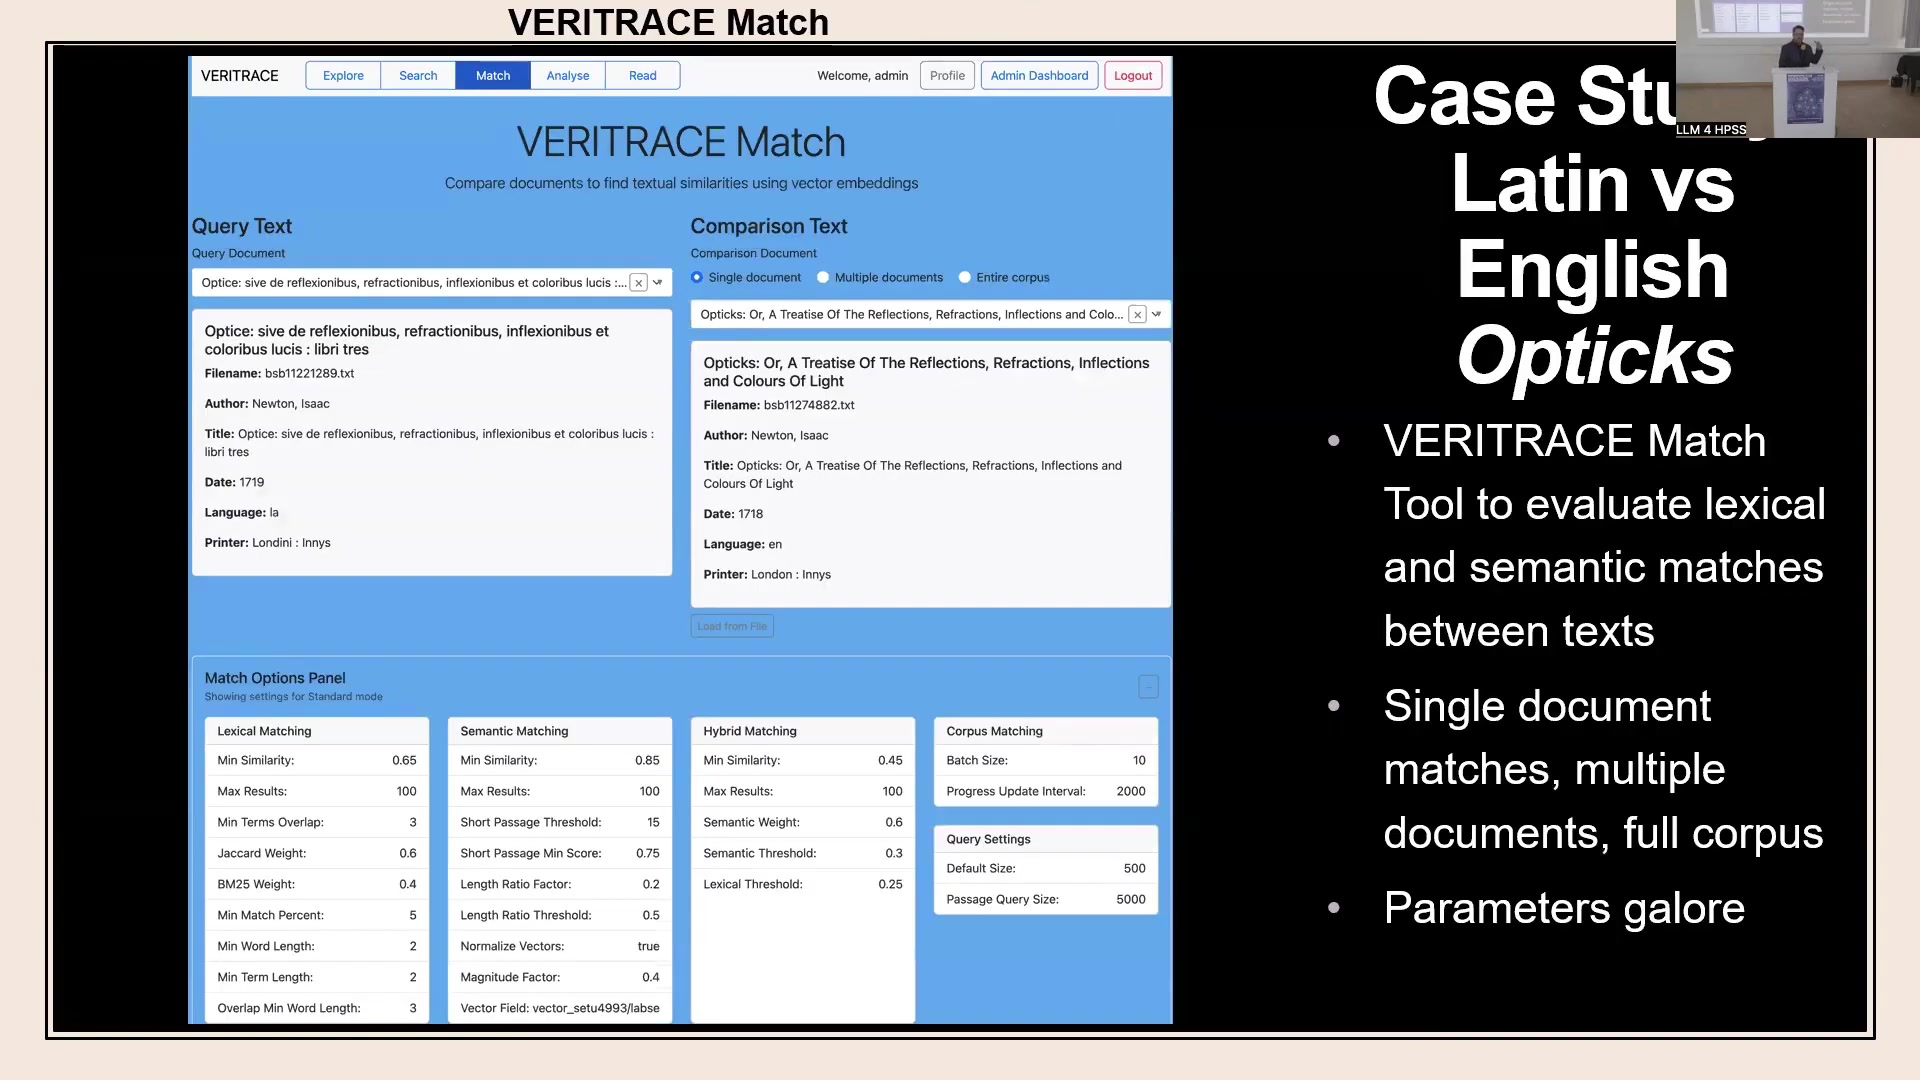
\includegraphics[keepaspectratio]{images/ai-nepi_006_slide_13.jpg}}

}

\caption{The VERITRACE `Analyse' interface showing planned analysis
tools.}

\end{figure}%

Recognising the importance of accessing original source materials, a
`Read' section integrates a Mirador viewer. This allows scholars to view
PDF facsimiles of every text in the corpus, alongside its metadata,
mirroring the experience of browsing a physical library's digital
collection.

\begin{figure}[H]

{\centering \pandocbounded{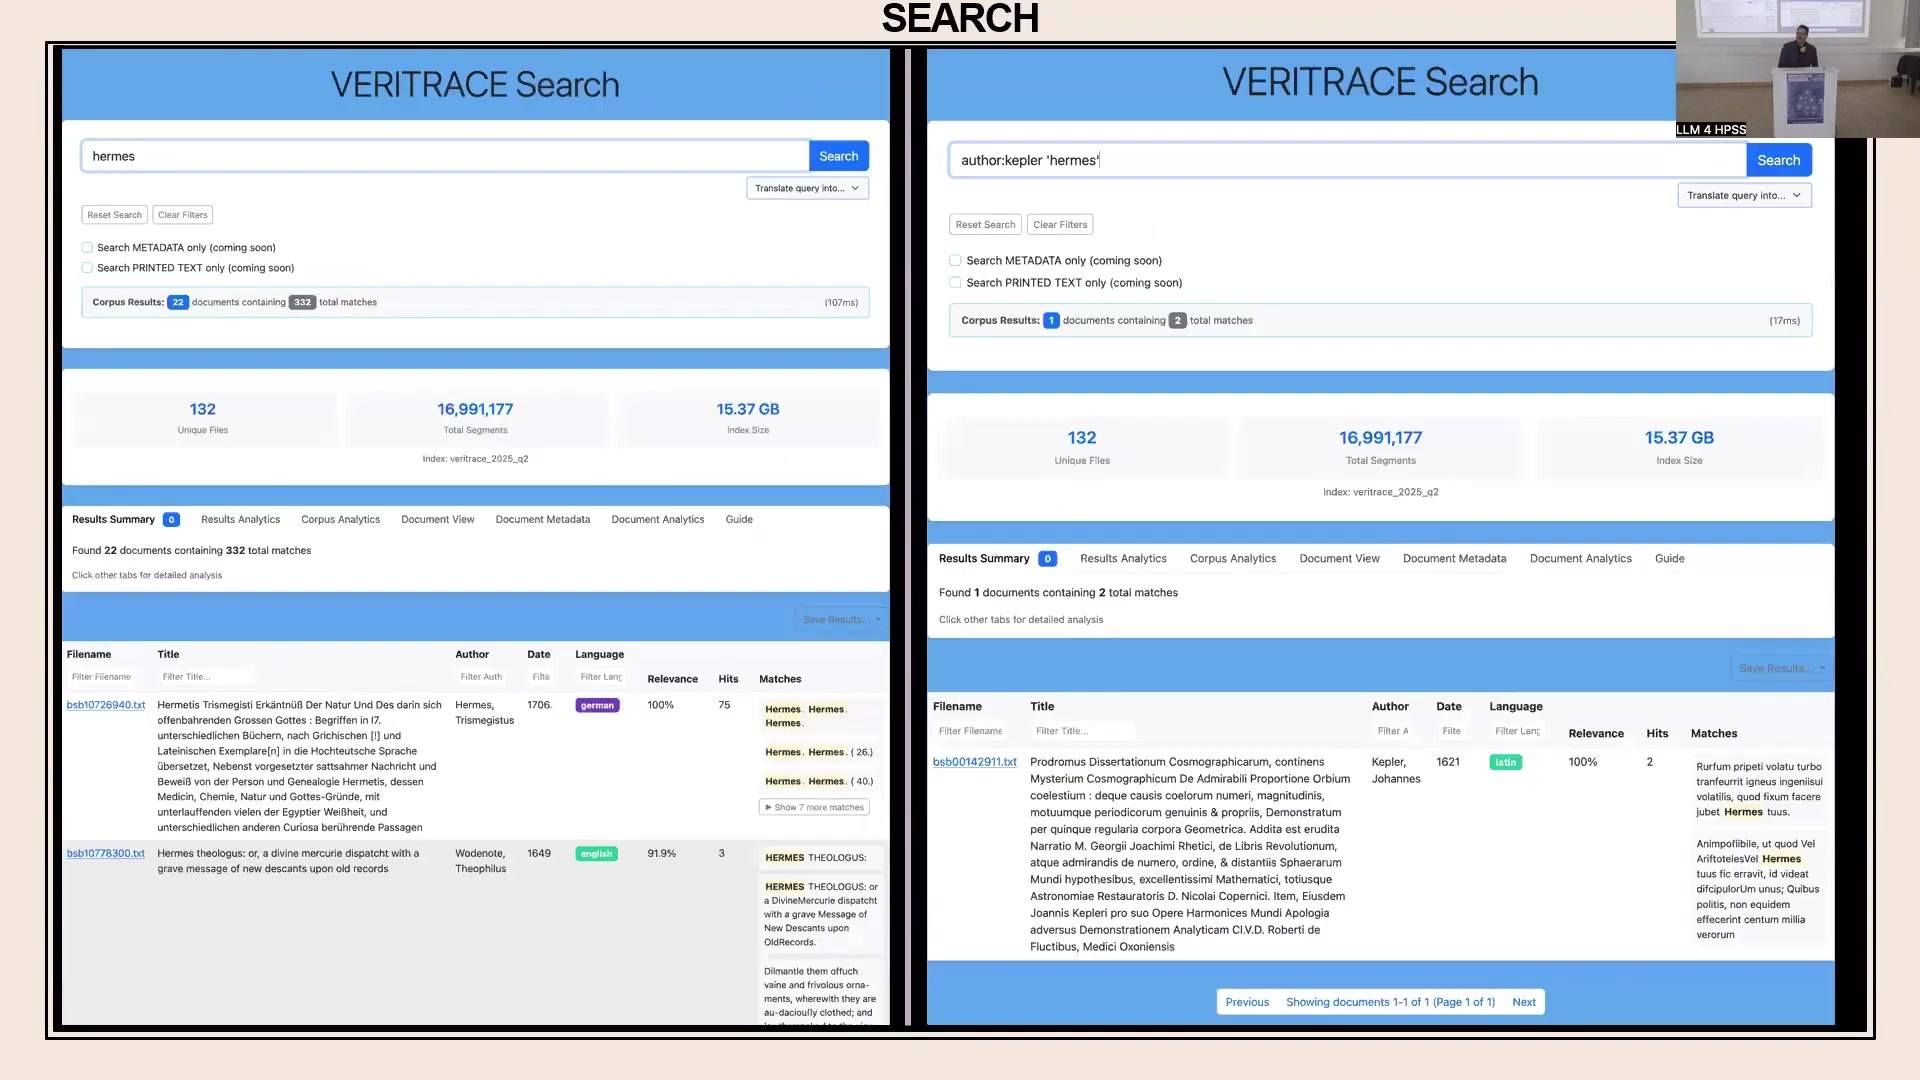
\includegraphics[keepaspectratio]{images/ai-nepi_006_slide_14.jpg}}

}

\caption{The VERITRACE `Read' interface with an integrated Mirador
viewer for text facsimiles.}

\end{figure}%

\section{Unveiling Textual Reuse: The Match
Functionality}\label{unveiling-textual-reuse-the-match-functionality}

A cornerstone of the VERITRACE web application is its `Match' section,
designed to identify textual reuse between different works. This tool
allows users to specify query texts and comparison texts. Comparisons
can be performed between single documents, across multiple selected
documents (e.g., comparing Newton's Latin \emph{Opticks} to all of
Kepler's works in the database), or, ambitiously, between one text and
the entire corpus. The latter presents considerable computational
challenges regarding processing time and user experience, but remains a
developmental goal.

\begin{figure}[H]

{\centering \pandocbounded{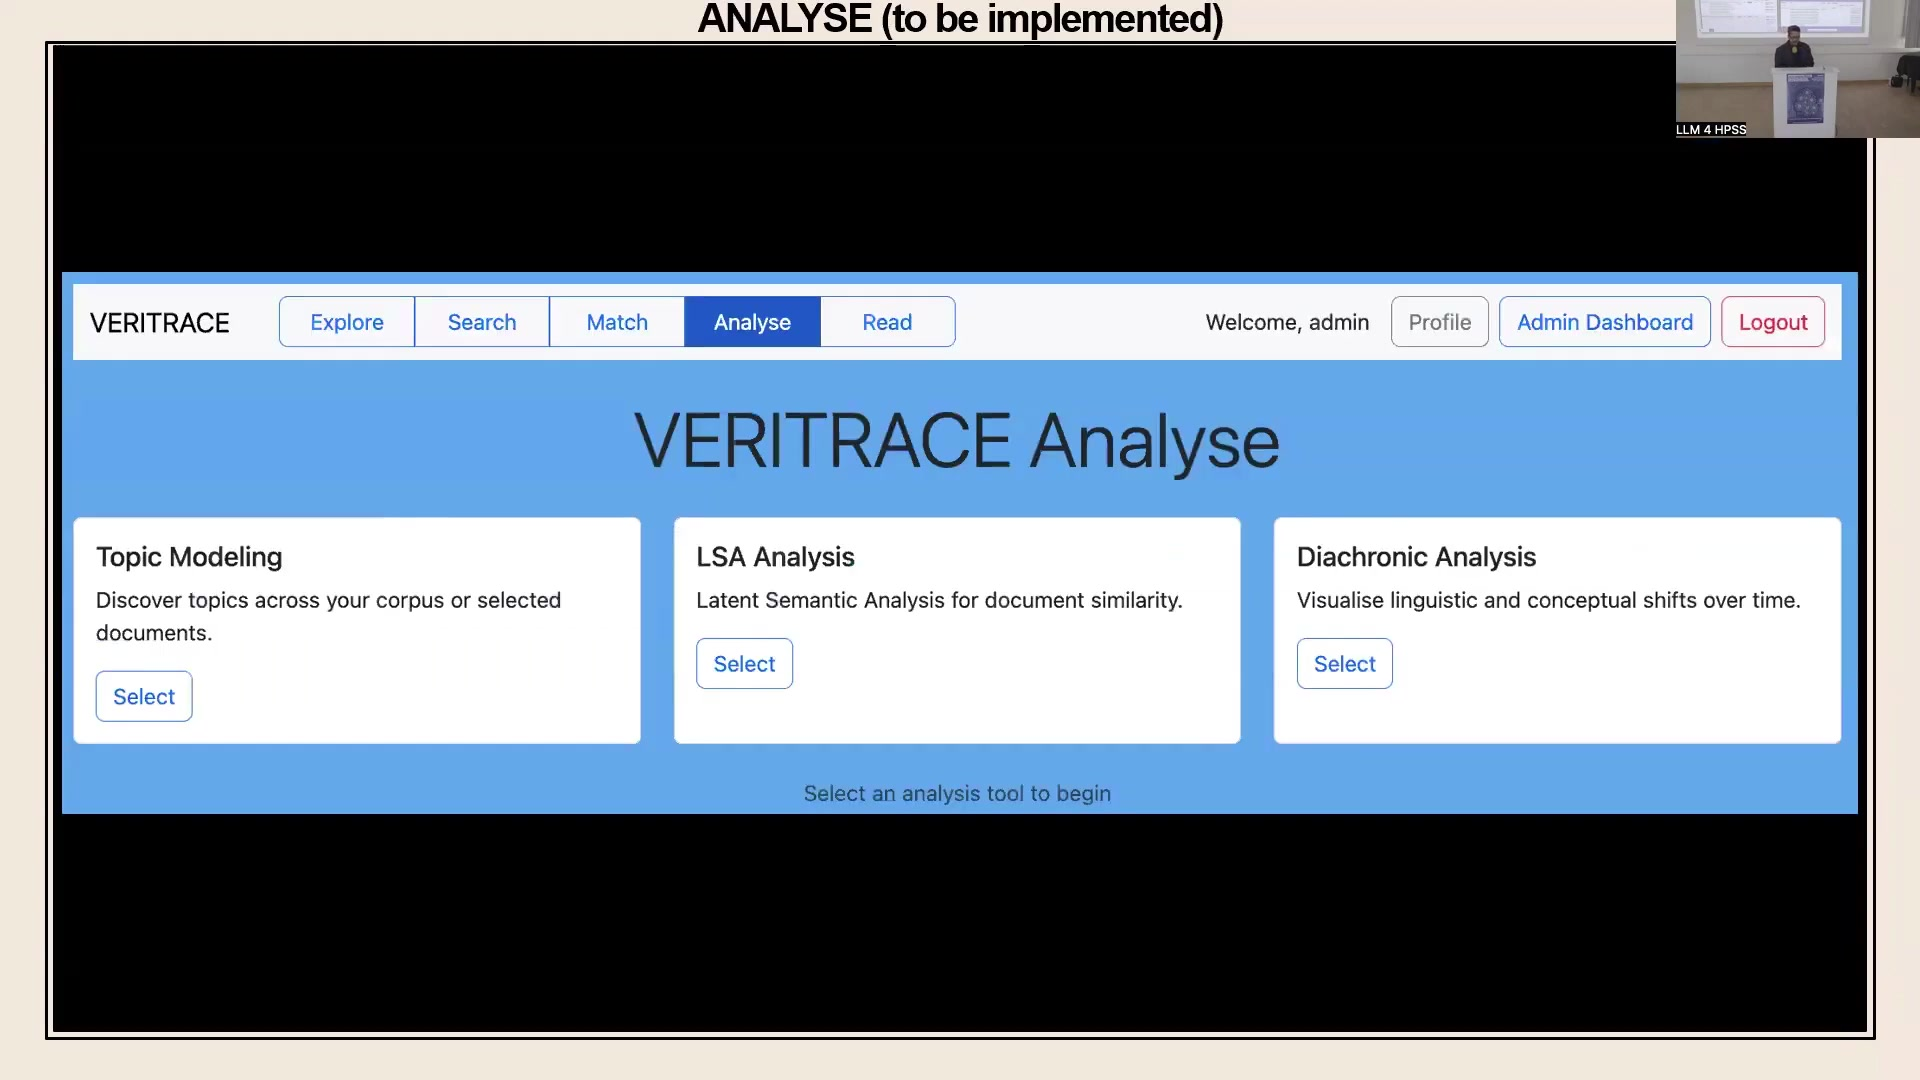
\includegraphics[keepaspectratio]{images/ai-nepi_006_slide_15.jpg}}

}

\caption{The VERITRACE `Match' interface for configuring textual
similarity comparisons.}

\end{figure}%

\subsection{Lexical and Semantic Matching
Approaches}\label{lexical-and-semantic-matching-approaches}

The system offers two fundamental types of matching:

\begin{enumerate}
\def\labelenumi{\arabic{enumi}.}
\item
  Lexical matching: This approach uses keyword-based techniques to find
  passages with similar vocabulary. It is effective for identifying
  direct textual parallels but is language-dependent.
\item
  Semantic matching: Employing vector embeddings, this method seeks
  conceptually similar passages, even if they share little or no common
  vocabulary. This is crucial for a multilingual corpus where
  translations or paraphrases might obscure lexical links.
\end{enumerate}

Hybrid approaches, combining lexical and semantic methods with
adjustable weighting, are also available.

\subsection{Customisable Parameters for Nuanced
Analysis}\label{customisable-parameters-for-nuanced-analysis}

Recognising that text matching is not a one-size-fits-all process, the
interface exposes numerous parameters for users to tweak. Whilst default
settings provide a balanced starting point, users can adjust elements
such as minimum similarity scores to refine search results according to
their specific research needs. Different matching modes---`Standard',
`Comprehensive' (for maximum recall, albeit slower), and `Faster' (for
higher precision with potentially fewer results)---offer further control
over the comparison process.

\section{Validating the Approach: Sanity Checks and Case
Studies}\label{validating-the-approach-sanity-checks-and-case-studies}

To evaluate the efficacy of the matching tools, researchers conduct
several `sanity checks' using known textual relationships. One such
check involves comparing Newton's Latin version of his \emph{Opticks}
(1719 edition) with the English edition from 1718. These texts, being
translations of each other, provide a useful test case.

\subsection{Sanity Check 1: Lexical Matching Across
Languages}\label{sanity-check-1-lexical-matching-across-languages}

When a lexical match is performed between the Latin and English editions
of \emph{Opticks}, the expectation is that no significant matches will
be found, given their different languages. Using the `Standard' matching
mode, this holds true---no matches are reported. Interestingly, the
`Comprehensive' mode does identify three matches, revealing small
sections of English text, likely from prefatory material, within the
predominantly Latin edition. This demonstrates the sensitivity of
different modes and confirms the general principle that lexical matching
is language-specific.

\begin{figure}[H]

{\centering \pandocbounded{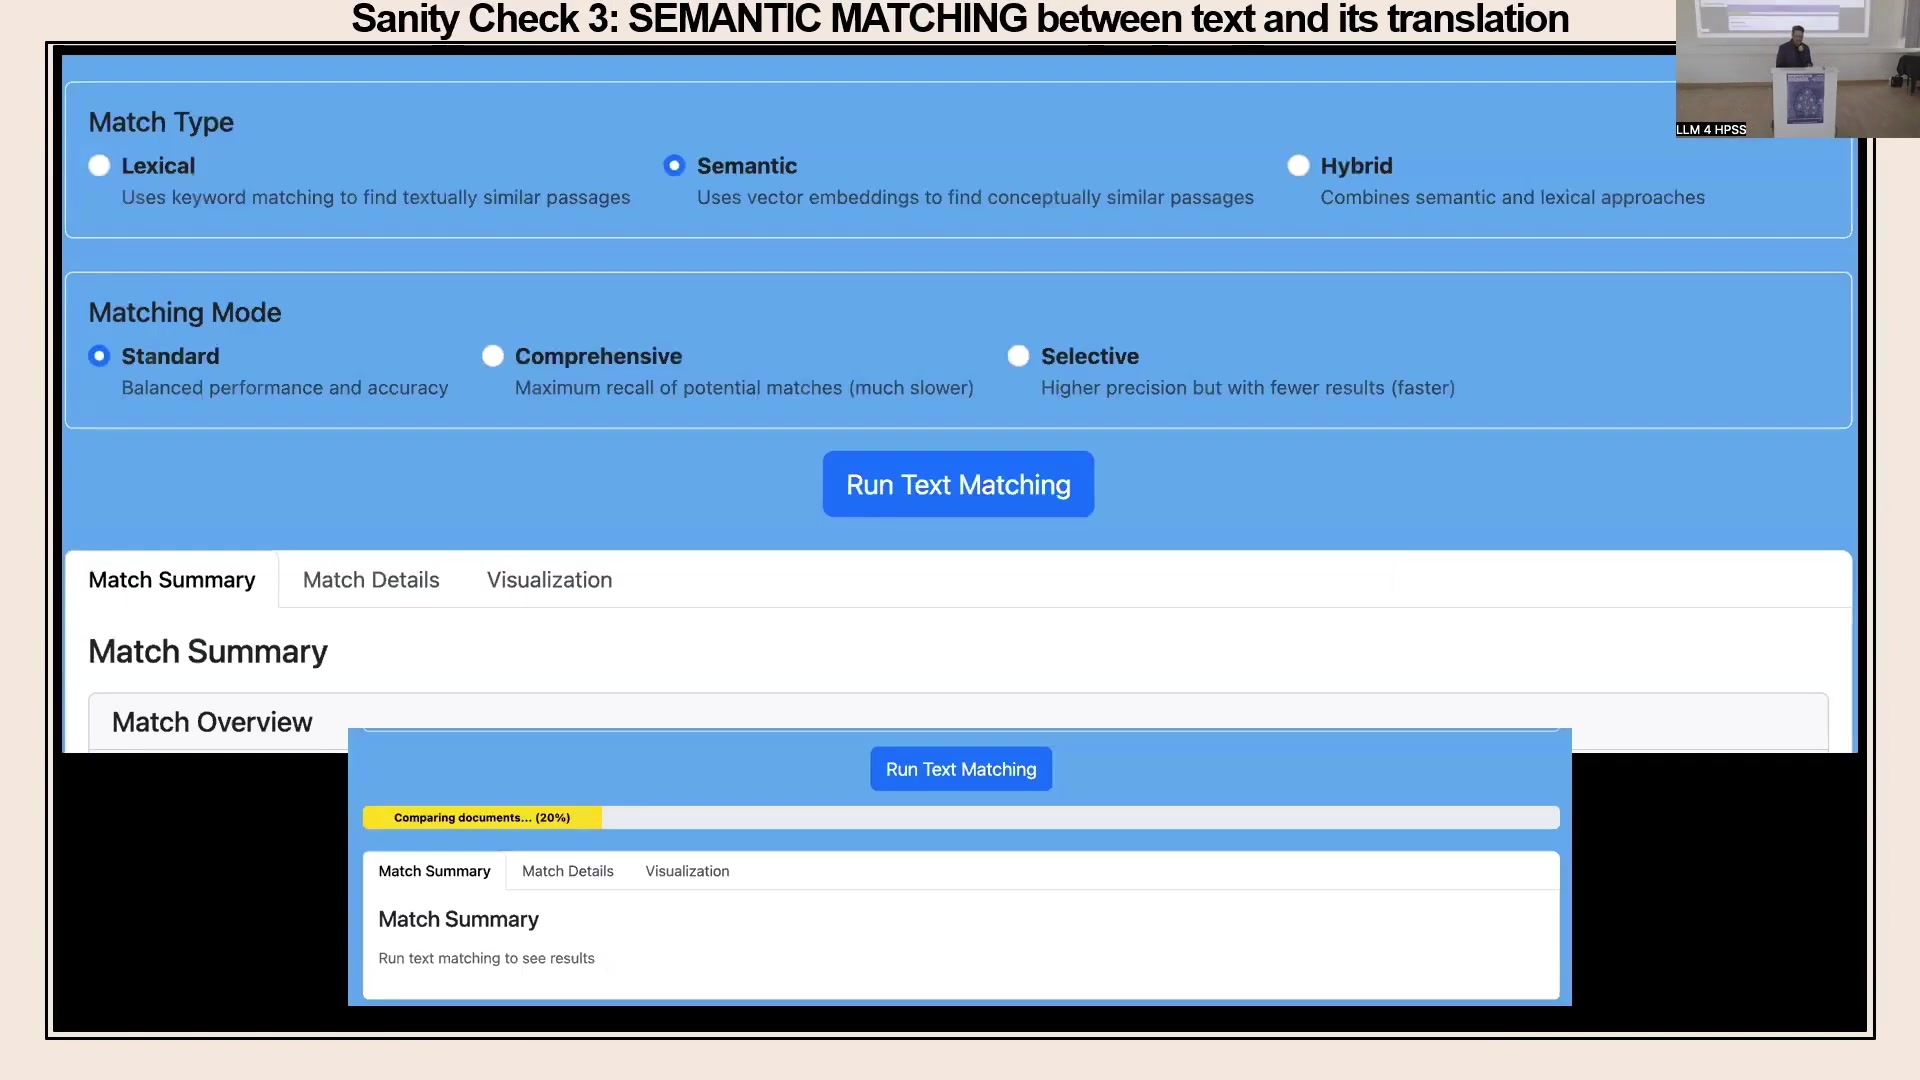
\includegraphics[keepaspectratio]{images/ai-nepi_006_slide_16.jpg}}

}

\caption{Results of a lexical match attempt between Latin and English
versions of Newton's Opticks, showing no significant matches.}

\end{figure}%

\subsection{Sanity Check 2: Lexical
Self-Matching}\label{sanity-check-2-lexical-self-matching}

As another baseline, lexically matching a text against itself should,
ideally, yield near-perfect results. When Newton's English
\emph{Opticks} is compared to itself, the system reports a high degree
of similarity, with extensive coverage and quality scores. The interface
provides detailed statistics, including the number of passages compared
and the distribution of similarity scores, offering transparency into
the matching process. Automatic highlighting displays the query passage
on the left and the comparison passage on the right, along with their
similarity score.

\begin{figure}[H]

{\centering \pandocbounded{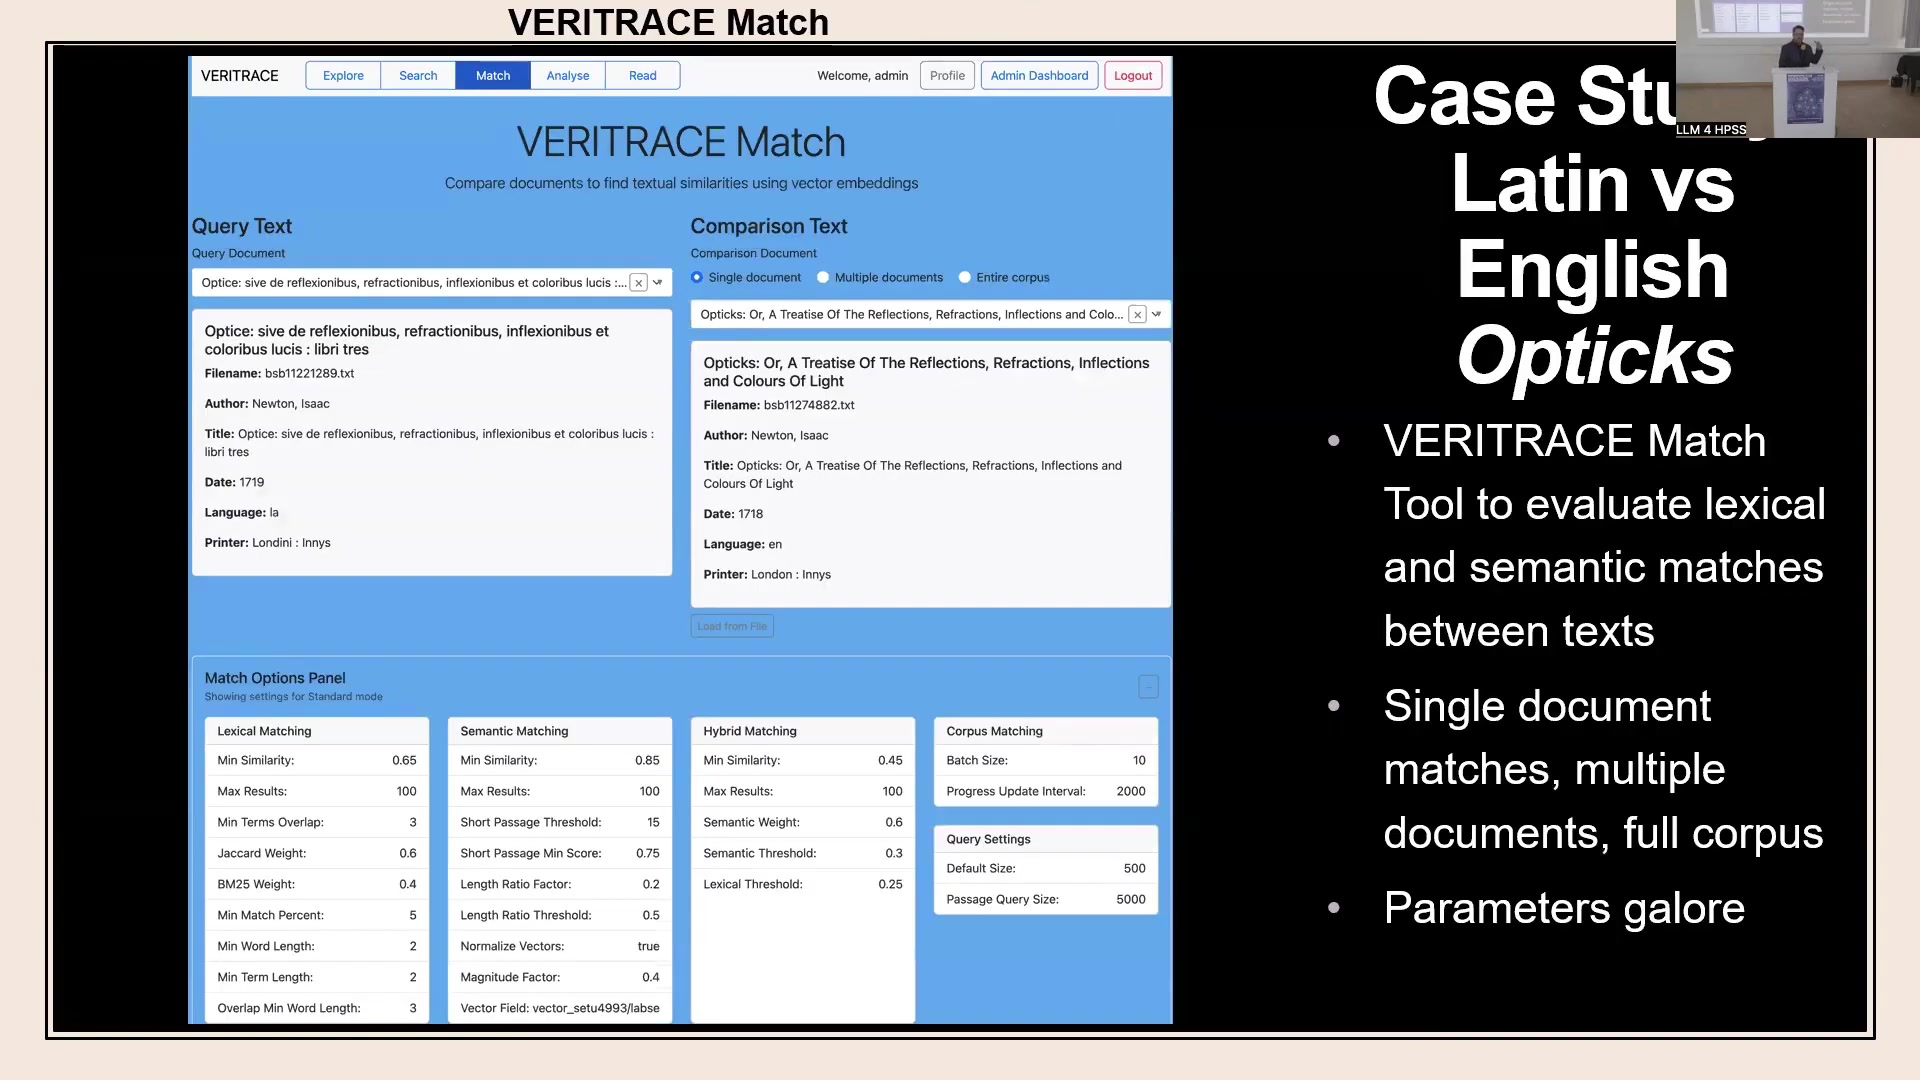
\includegraphics[keepaspectratio]{images/ai-nepi_006_slide_17.jpg}}

}

\caption{Results of lexically matching Newton's Opticks to itself,
showing high similarity.}

\end{figure}%

\subsection{Sanity Check 3: Semantic Matching of
Translations}\label{sanity-check-3-semantic-matching-of-translations}

The real test for the LLM-powered tools comes with semantic matching
across languages. When comparing the Latin and English \emph{Opticks}
using semantic matching, the system should identify conceptual
similarities despite the linguistic differences.

\begin{figure}[H]

{\centering \pandocbounded{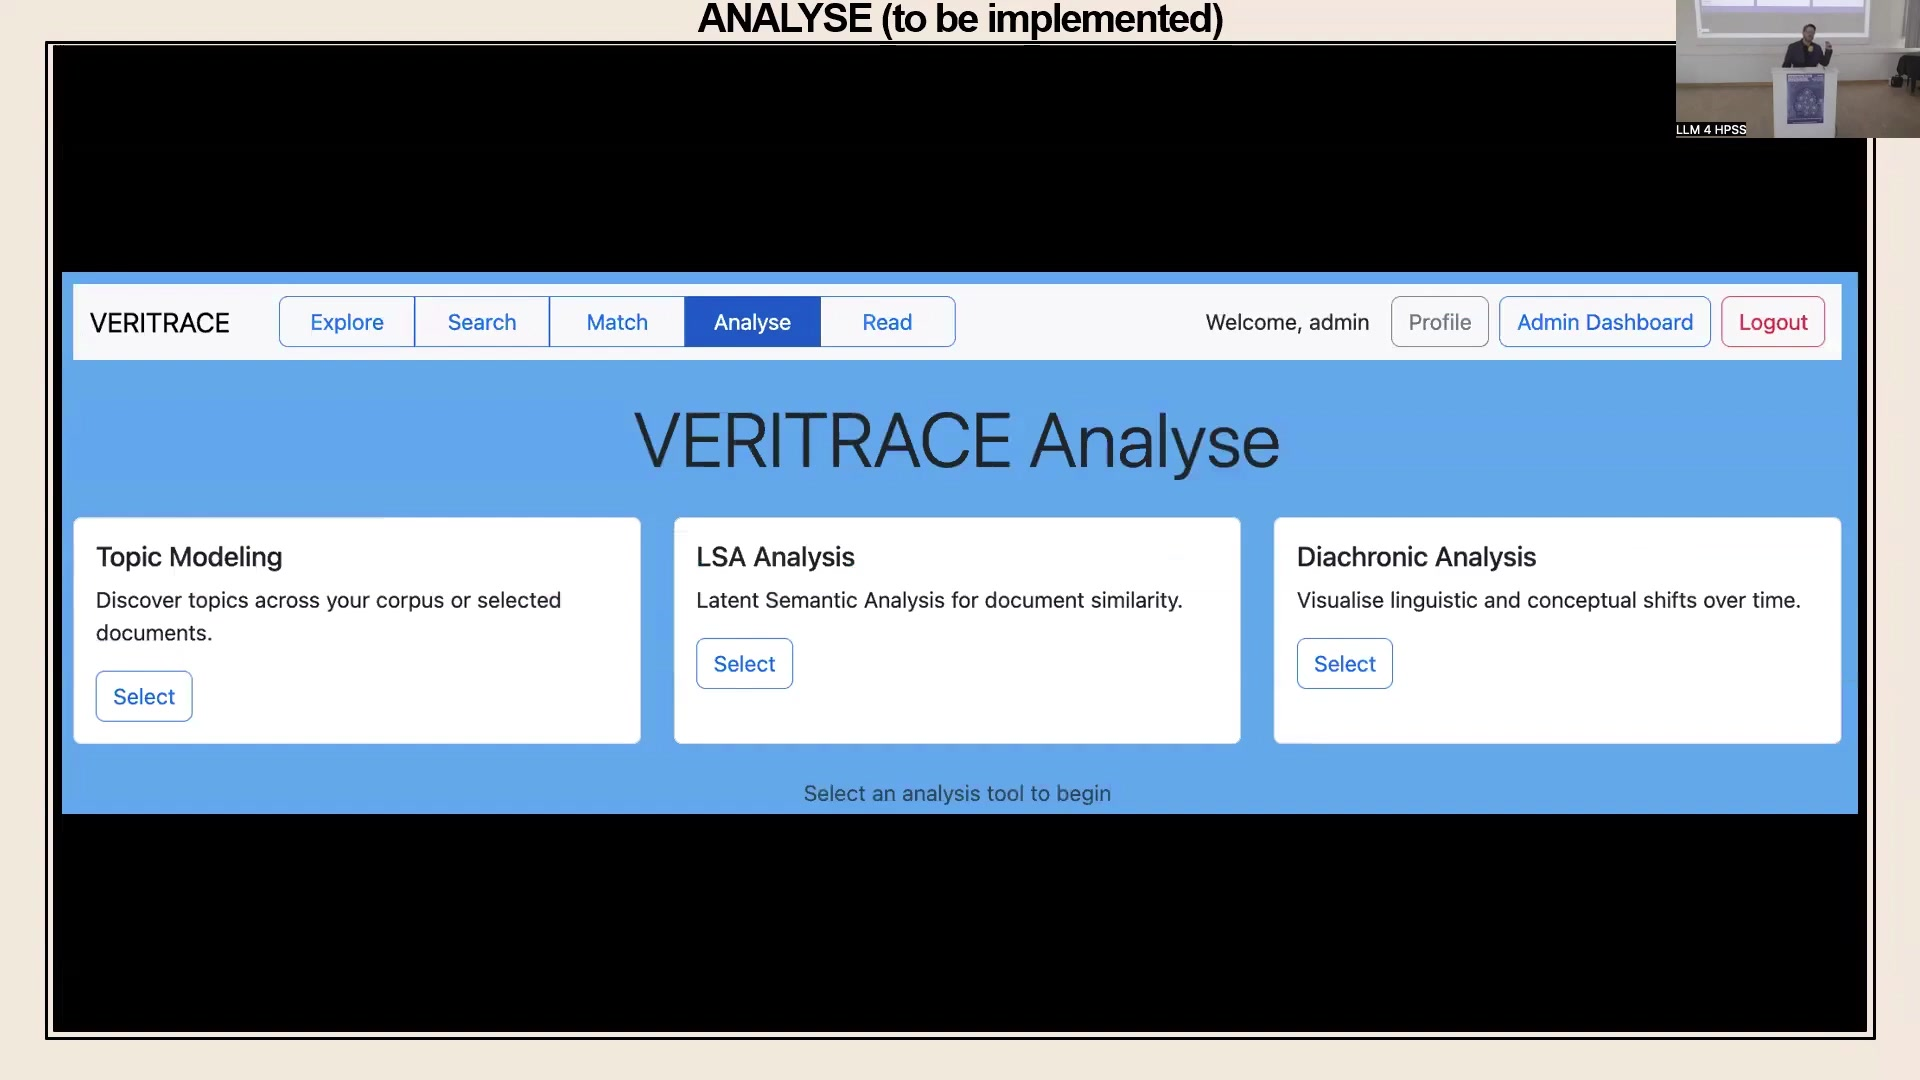
\includegraphics[keepaspectratio]{images/ai-nepi_006_slide_18.jpg}}

}

\caption{Configuration for a semantic match between Newton's Latin
Optice and its English translation.}

\end{figure}%

Initial results from such semantic comparisons appear reasonable.
Passages discussing similar concepts, such as colours, are identified as
matches, even with underlying OCR imperfections. This suggests that the
vector embeddings are capturing some level of conceptual correspondence
across translations.

\begin{figure}[H]

{\centering \pandocbounded{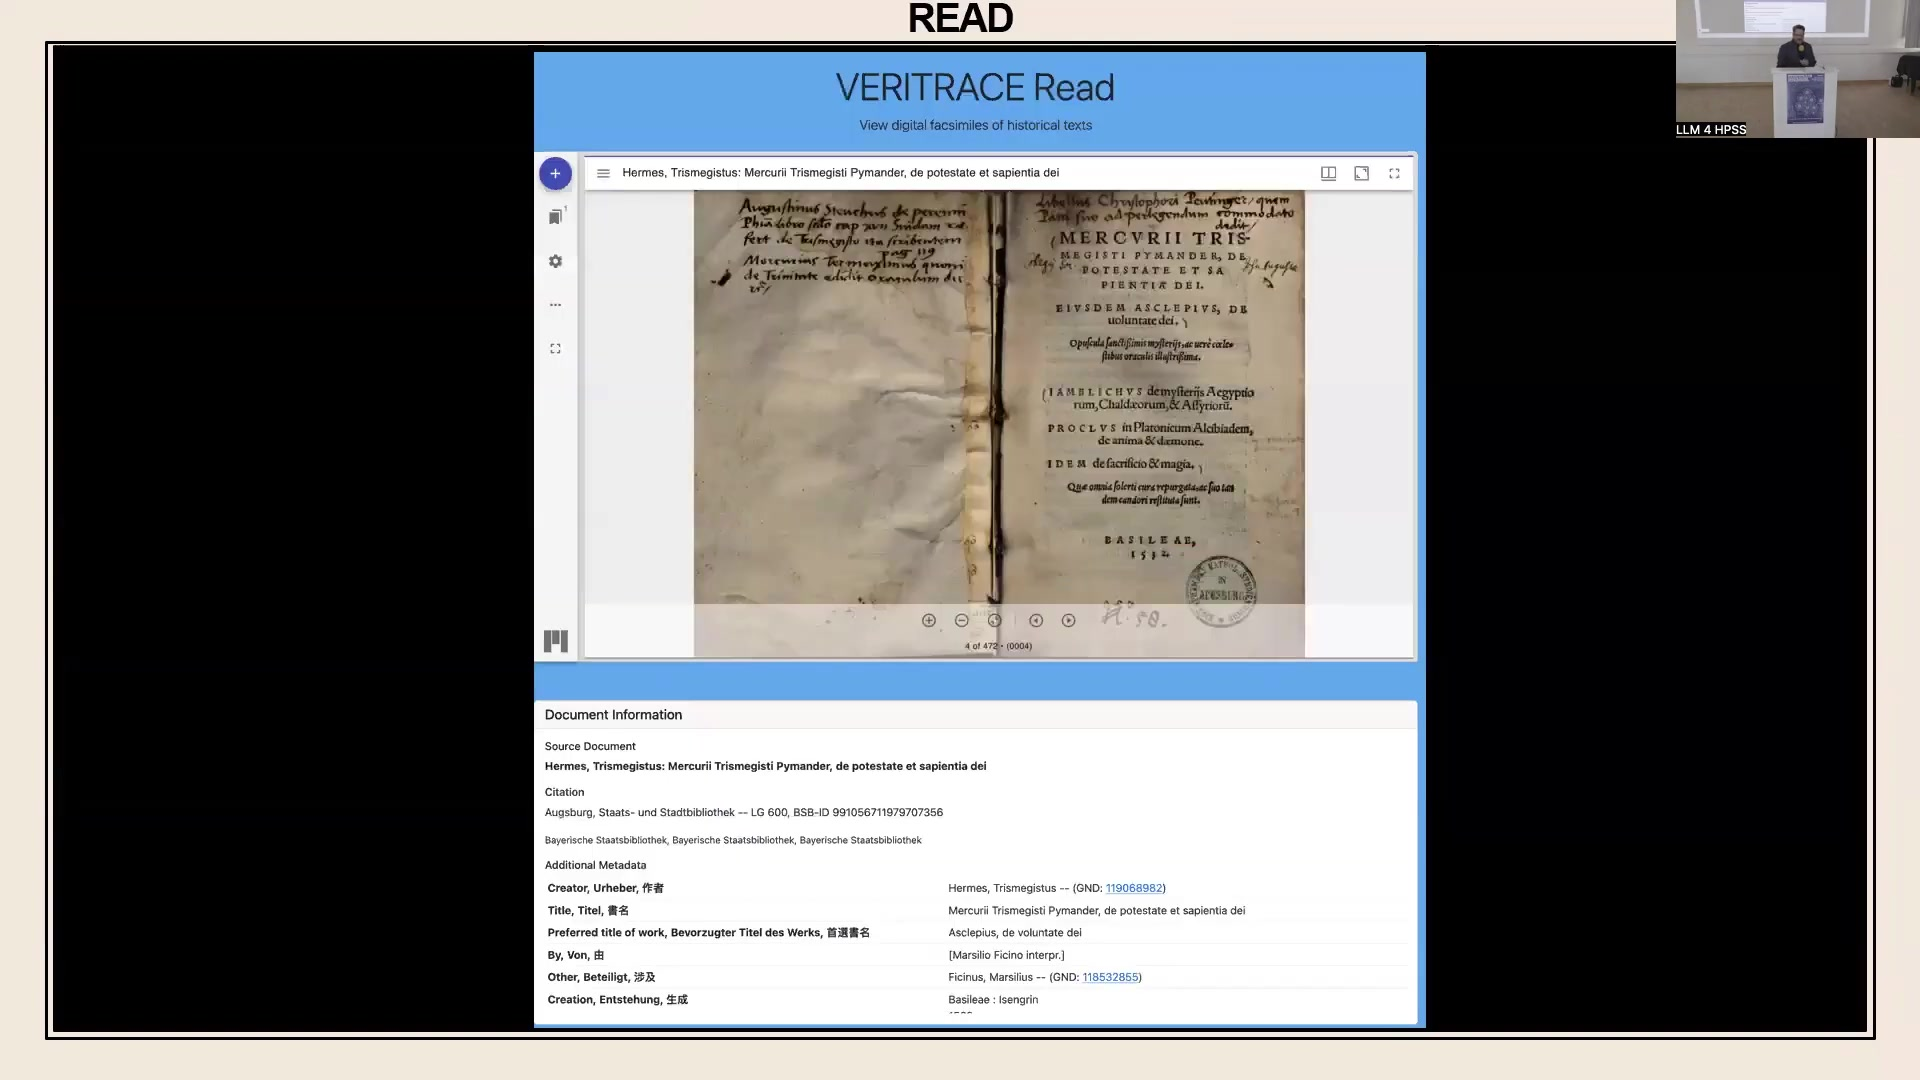
\includegraphics[keepaspectratio]{images/ai-nepi_006_slide_19.jpg}}

}

\caption{Examples of semantic matches found between Latin and English
versions of Newton's Opticks.}

\end{figure}%

\subsection{Preliminary Findings and Model
Adequacy}\label{preliminary-findings-and-model-adequacy}

However, the semantic matching performance is not without its issues.
Whilst the quality score for identified matches can be high, indicating
strong similarity for the pairs found, the coverage score---representing
how much of the documents are involved in matches---can sometimes be
lower than expected. This discrepancy might, in part, reflect genuine
differences between editions; for instance, the Latin edition of
\emph{Opticks} is considerably longer than the English one.

\begin{figure}[H]

{\centering \pandocbounded{\includegraphics[keepaspectratio]{images/ai-nepi_006_slide_20.jpg}}

}

\caption{Summary statistics for the semantic match between Latin and
English Opticks, highlighting areas for investigation.}

\end{figure}%

Nevertheless, further queries using the current LaBSE embedding model
suggest it may not be entirely adequate for the nuanced demands of
historical textual analysis. The potential for `out-of-domain model
collapse'---where a model trained on general modern text performs poorly
on specialised historical corpora---is a concern.

\section{Future Directions and Outstanding
Challenges}\label{future-directions-and-outstanding-challenges}

As the VERITRACE project progresses, several critical issues and areas
for development lie on the horizon. The choice of vector embedding model
is paramount. LaBSE, selected partly for its efficiency in terms of
storage and processing speed, may prove insufficient. Alternative
models, such as XLM-Roberta, intfloat multilingual-e5-large, or
specialised historical mBERT variants, present other trade-offs between
accuracy, storage requirements, and inference time. A fundamental
question is whether to persist with pre-trained models or to invest in
fine-tuning a base model specifically on the VERITRACE historical
corpus.

\begin{figure}[H]

{\centering \pandocbounded{\includegraphics[keepaspectratio]{images/ai-nepi_006_slide_21.jpg}}

}

\caption{A summary of key issues and future challenges for the VERITRACE
project.}

\end{figure}%

Further challenges include:

\begin{itemize}
\item
  Semantic drift: The meaning of words and concepts changes over time.
  How effectively current LLMs handle such diachronic semantic shifts
  across centuries and languages within the same vector space remains an
  open question.
\item
  OCR quality: Poor OCR accuracy profoundly impacts downstream tasks,
  from basic sentence segmentation to complex semantic analysis.
  Re-OCRing the entire corpus is not feasible. Strategies might involve
  selectively re-OCRing the poorest quality texts or investing effort in
  locating existing higher-quality digital versions.
\item
  Scaling and performance: The current prototype, operating on only 132
  texts, already shows query times of around 15 seconds for complex
  operations. Scaling these capabilities to the full corpus of 430,000
  texts will undoubtedly present significant performance engineering
  challenges.
\end{itemize}

Addressing these multifaceted issues will be crucial for realising the
full potential of VERITRACE to illuminate the complex intellectual
heritage of early modern science. Continued research, methodological
refinement, and community engagement will guide these future endeavours.

\bookmarksetup{startatroot}

\chapter{---}\label{section-3}

\begin{center}\rule{0.5\linewidth}{0.5pt}\end{center}

\bookmarksetup{startatroot}

\chapter{---}\label{section-4}

\bookmarksetup{startatroot}

\chapter{References}\label{references}

\bookmarksetup{startatroot}

\chapter{References}\label{references-1}

\{.unlisted\}


\backmatter


\end{document}
